\documentclass[a4paper, 11pt]{book}

%\usepackage[latin1]{inputenc}
%\usepackage[ansinew]{inputenc}
%\usepackage[utf8]{inputenc}
%\usepackage{ucs}


% Note and error commands for correction purposes. 
\newcommand{\notiz}[1]
{\marginpar{\small\blue #1}}
\newcommand{\fehler}[1]
{\marginpar{\small\red #1}}



\usepackage[utf8x]{inputenc}
\usepackage[T1]{fontenc}
%\pdfmapfile{+FrutigerCom.map} % geht auch ohne
% There needs to be a fix and message to use frutiger if present!
%\usepackage[light,bold]{FrutigerCom}

\usepackage[pdftex]{graphicx}
\usepackage[english]{babel}
\usepackage{amsmath}
\usepackage{amssymb}%include things such as \mathbb{}
\usepackage{hyperref}
%\usepackage{units}
\usepackage{framed, color}
\usepackage{listings}

\usepackage{siunitx}
\usepackage{booktabs} % nicer rules in tabular


\usepackage{pstricks}
\usepackage{ifthen} %required for variable arguments in newcommand

%%% This is where to switch between final and developers version!
\newboolean{draft}
\setboolean{draft}{true}

\ifthenelse{\boolean{draft}}
{\newcommand{\todo}[2][\empty]{\ifthenelse{\equal{#1}{\empty}}{\emph{\color{red} TODO:} \emph{#2}\index{TODO: #2}}{\emph{\color{red} TODO:} \emph{#2}\index{TODO: #1}}}}
{\newcommand{\todo}[2][\empty]{\ifthenelse{\equal{#1}{\empty}}{}{}}}
\ifthenelse{\boolean{draft}}
{\newcommand{\fixme}[2][\empty]{\ifthenelse{\equal{#1}{\empty}}{\emph{\color{red} FIXME:}\emph{#2}\index{FIXME: #2}}{\emph{\color{red} FIXME:}\emph{#2}\index{FIXME: #1}}}}
{\newcommand{\fixme}[2][\empty]{\ifthenelse{\equal{#1}{\empty}}{}{}}}
\ifthenelse{\boolean{draft}}
{\newcommand{\draft}[1]{#1} }
{\newcommand{\draft}[1]{} }
\ifthenelse{\boolean{draft}}
{\usepackage{draftwatermark}
\SetWatermarkText{\textbf{Internal Use Only}}
\SetWatermarkScale{ 2 }
\SetWatermarkLightness{0.85}
}
{}

\lstset{backgroundcolor=\color{gray!20},
  basicstyle=\ttfamily,
  basicstyle=\small,
  breakindent=0pt,
  breaklines=true, %Allows line breaking for long lines
  breakatwhitespace=true, %Only break on whitespace
  postbreak=\mbox{\textcolor{gray}{$\hookrightarrow$}\space\space\space},
  prebreak=\mbox{\textcolor{gray}{$\backslash$}}
}

% siunitx in MikTeX 2.9 already defines angstrom and ua
\providecommand{\angstrom}{\text{\normalfont\AA}}
\providecommand{\astronomicalunit}{\text{ua}}
% strange name clash with siunitx
\newcommand{\siday}{\text{d}}
\newcommand{\siyear}{\text{a}}

\newcommand{\laplace}{\triangle}

\usepackage{makeidx}
\makeindex{}

% Deckblatt
\date{\today}
\title{
  \vspace{-3ex}
  
\includegraphics[width=0.75\textwidth]{visuals/tremolo-x.png}\\
  \vspace{3ex}
Tremolo-X Manual\footnote{
    Tremolo-X, TremoloGUI is
    Copyright \copyright 2010-2013 Fraunhofer Institute for Algorithms and Scientific Computing SCAI.
    All rights rserved.
    It is not permitted to copy or distribute this product or any parts of it.
  }\\ {(Version 1.6)}}
\author{{\Large{}\bf Fraunhofer SCAI}\\
\\
For questions, errors and updates please contact:\\
Christian Neuen\\
christian.neuen@scai.fraunhofer.de\\
\\
Contributors:\\
Gregor Bollerhey\\
Dr. Jan Hamaekers\\
Christian Neuen\\
Ralph Thesen\\
\\
Thanks go to:\\
Lukas Jager\\
Ralf Wildenhues
}

\begin{document}

\maketitle

\todo{Recompile with frutiger font if available!}
%\cleardoublepage
\printindex

\setcounter{tocdepth}{2}

\tableofcontents
%\cleardoublepage
%\pagestyle{empty}
%\null\newpage
%\pagestyle{empty}
%\null\newpage

\chapter{Overview}

\todo{Check urls in bibliography (obtained from (very) old comments!!!}

This is a user manual into the TREMOLO-X Molecular Dynamics simulation package.
Should you be interested in an in-depth introduction into the numerics of molecular dynamics simulation, you might want to read \cite{GriebelEng}
\bigbreak
For up-to-date news and other interesting information about the \mbox{TREMOLO-X} software, please visit:
\begin{center}
 \url{www.tremolo-x.com} 
\end{center}

Tremolo-X is a molecular dynamics simulation package. The program consists of two major components, which allow either sequential or parallel computation of the simulation.

Tremolo-X supplies a choice of several common bonded and non-bonded potentials, which can be combined in order to simulate systems which are dependent on intra- and intermolecular forces.

You may choose from a variety of statistical ensembles and boundary conditions, in order to tailor the simulation to your particular settings and needs.

Furthermore, the dynamic simulations may be augmented or replaced with energy optimization routines.

\section{How to read the manual}

This manual begins with a descriptions of the different capabilities (ensembles, integrators, thermostats,...) of the program, and their interdependencies. We tried to add as much mathematical detail as necessary, but as little as possible, however we always indicate a source, where you can find more details, when you are interested beyond the mere usability of the product.
We continue with an in-depth description of the different potentials you can specify in Tremolo-X and finish with a detailed specification the syntax of options in the parameter file.

\draft{\chapter{Configuration and Setup}}

\todo{How will the setup work for the enduser?}

\chapter{First steps}

{\small The first section of this chapter is identical to the Quickstartguide provided next to the manual. For a detailed description please read the rest of the manual. 
The second section mirrors the first, giving an example for the use of the parallel version.}
\bigbreak

\section{First sequential steps}
\label{Quickstart}

Switch to the Tremolo-X folder and enter the \texttt{example/Argon/} folder therein.
Have a glance at the files currently present in the directory.
Now type
\begin{lstlisting}
 tremolo argon.tremolo
\end{lstlisting}
Congratulations! You are running your first Tremolo-X simulation!
\bigbreak
Now that did not look like there was much happening, did it? So let's try that again and have tremolo generate some more output:
\begin{lstlisting}
 tremolo -v argon.tremolo
\end{lstlisting}
While some of the information is self explanatory, some is not, so if you want to know about everything, have a look at the manual!

As soon as the program is finished and console command has been returned to you, have another look at the content of the directory. The additional files contain the measurements of Tremolo-X.
The files argon.e* contain information about the energy in the ensemble, e.g. in \texttt{argon.etot} you find the \textbf{total energy}, which remained constant through the simulation (of course there are some oscillations due to numeric effects). Similarly you find the \textbf{potential energy} in \texttt{argon.epot} and the \textbf{kinetic energy/temperature} in \texttt{argon.ekin}. 

Here, as in most output files, columns are printed for different particle groups, so if you have more than one type of particle in your simulation, more columns with the respective values will appear.

Opening the .msd file you find several columns which contains data towards the computation of the \textbf{diffusion coefficient(s)}, in particular in the column labeled \textit{Dif\_sum}. (Note that the numeric values are computed in reduced units, please refer to the manual.)

In most cases it is beneficial to look at a graph, instead of those long columns of numbers. If you have no favorite plotting program of your own, you could try gnuplot\footnotemark[1], it is free and fairly easy to use.
\bigbreak
The files \texttt{argon.vis.\#\#\#\#.[xyz,pdb,data]} contain the \textbf{positions} (and also other data) of the atoms at specific time points in the simulation, e.g. in \texttt{argon.vis.0100.[xyz,pdb,data]}, you find the positions at the end of the simulation. 

As before you might prefer to look at pictures instead of the numbers, so if you do not have a favorite program for visualizing .xyz or .pdb output, you could try vmd or ovito\footnotemark[1], as it is also free and easy to use. 
\footnotetext[1]{Neither gnuplot, nor vmd, nor ovito are developed, maintained, distributed or in any other way associated with Fraunhofer SCAI.}



\section{First parallel steps}
\label{FirstParallelSteps}

Switch to the Tremolo-X folder and enter the example/Argon folder therein.
Have a glance at the files currently present in the directory.
Now type
\begin{lstlisting}
 mpirun -np 8 tremolo_mpi -p 2,2,2 argon.tremolo
\end{lstlisting}
Congratulations! You are running your first parallel Tremolo-X simulation!
\bigbreak
As before, you will obtain more output with the verbosity option by typing
\begin{lstlisting}
 mpirun -np 8 tremolo_mpi -p 2,2,2 -v argon.tremolo
\end{lstlisting}

As soon as the program is finished and console command has been returned to you, have another look at the content of the directory. The additional files contain the measurements of Tremolo-X.
The files argon.e* containing the energy measurements appear as they did in the serial case and are organized in the same way.

\bigbreak
What changed are the output files for the visualization (.xyz and .pdb) and the data state file (.data.9999).
Instead of {\tt argon.vis.\#\#\#\#.xyz} ({\tt argon.vis.\#\#\#\#.pdb}) you find {\tt argon.vis.\#\#\#\#.\#\#\#\#.xyz} ({\tt argon.vis.\#\#\#\#.\#\#\#\#.pdb}), similarly you see {\tt argon.data.9999.\#\#\#\#} files.
This is due to the fact that all processes write output for their segment simultaneously to speed up the process.
In order to combine these segments, an easy to use tool is provided in the utility section of tremolo.

Typing
\begin{lstlisting}
 /PATH_TO_TREMOLO_BINARIES/MergeOutput.py argon xyz
\end{lstlisting}
will combine the separate xyz files and produce a unified one for the complete domain of the simulation. Adding the option {\tt -d} will cause the original, partial files to be deleted. Similarly
{\tt pdb} and {\tt data} files can be merged by typing 
\begin{lstlisting}
 /PATH_TO_TREMOLO_BINARIES/MergeOutput.py argon pdb
\end{lstlisting}
or 
\begin{lstlisting}
 /PATH_TO_TREMOLO_BINARIES/MergeOutput.py argon data
\end{lstlisting}
respectively. For more options type 
\begin{lstlisting}
/PATH_TO_TREMOLO_BINARIES/MergeOutput.py -h
\end{lstlisting}

Visualization of those files functions exactly as described for the serial case. (For the use of the {\tt .data.9999} file please refer to the manual.)

\chapter{Running Tremolo}
\label{running_tremolo}

Tremolo-X allows two distinct modes of operation: Control from a command line, which allows the user to take advantage of scripts for task automation, and control from a graphical user interface, which provides an interactive environment and relieves the user of the burden to handle the parameter syntax.

\section{Command line}

Assuming, the Tremolo-X installation path belongs to the \$PATH environment of your system,
the most basic command to call (serial) tremolo is 
\begin{lstlisting}
 tremolo project.tremolo
\end{lstlisting}

In order to call the parallel version, the call is modified to 
\begin{lstlisting}
 tremolo_mpi project.tremolo
\end{lstlisting}

Both versions share the following parameters:
% The debug parametes will only be shown in the internal version.
\begin{lstlisting}
Usage: tremolo [-hvx ] [-a alarmtime] [-d debugstr|-D debugstr] [-n nicelevel] [-o verbosity] [-s sleeptime] [-f] mainparameterfile
  -a alarmtime  Sets alarm to alarmtime seconds. Code will finish after next timestep, writing out the current state.
  -f mainfile   Specify main parameter file (last argument: '-f' may be omitted)
  -h            Displays this help page and exits successfully.
  -n nicelevel  Decreases priority of process.
  -v            Increases verbosity level by one. Default value: 0.
  -V            Print version.
\end{lstlisting}

\draft{
Only for developers and in developer version the following options are accepted:
%\begin{lstlisting}
{\tt  -d debugstr   Starts debugger right away.

  -D debugstr   Starts debugger when encountering an error.
                Valid syntax for debugstr:
                0 sleep for a minute, no debugger
                [host[:display][,debugger]]  start debugger xterm on host:display
                (if DISPLAY is set or for local connection set host to local).
                Valid values for debugger are: gdb, dbx, ddd, cvd, totalview, ups.

  -s sleeptime  wait sleeptime seconds for debugger to come up (-d, -D)}
%\end{lstlisting}
\todo{Create new lst listing environment which is sensitive to the draft option}
}

\todo{detail verbosity syntax}

while the parallel version takes one additional parameter,
\begin{lstlisting}
  -p px,py,pz   Start parallel code with domain decomposition,
                using px slices on x-axis, py slices on y-axis and pz slices on z-axis (total: px*py*pz processes)
\end{lstlisting}
which must be supplied to actually benefit from parallel execution, since the default would be one process.
However, Tremolo-X will always check whether the number of processes in the MPI-call matches the number
of sub domains in the domain decomposition and will throw an error if this is not the case.


For parallel codes it may be necessary to specify the main parameter file
with an absolute path.

\draft{
\section{Using the GUI}

\todo{separate instructions for the GUI?}
}

\chapter{Domain and Boundaries}
\label{domain}

The first step of setting up a Molecular Dynamics simulation is to decide and specify the domain of the system. The domain is determined by its shape and the type of boundary, e.g. what happens, when a particle crosses the boundary domain. Several choices are available in Tremolo-X which, depending on the setup desired, can be combined freely.
The shape of domain used determines the type of input required: 

\begin{itemize}
 \item A \textit{cube}(={\tt cube}) requires only one parameter, an edge length.
\item A \textit{cuboid}(={\tt diag}) requires three edge length.
\item A \textit{parallelepiped}(={\tt matrix}) requires its complete matrix, i.e. the collection of the three edge vectors. The vectors are written column wise in the matrix, i.e. each column corresponds to one box-vector. (xx, xy and xz are first vector and so on).
\end{itemize}

Note that one can also give the box matrix by a \texttt{\# BOX} line
in the \texttt{.data} file. In particular, a \texttt{\# BOX} line
given in the \texttt{.data} file will overwrite values from the
\texttt{.parameter} file.

\bigbreak

The boundary conditions have a direct correspondence to the simulated physical environment of sample.
\begin{itemize}
 \item \textit{Reflecting} boundary conditions are self-describing, momentum is preserved. % Checked.
 \item \textit{Leaving} boundary conditions allow particles to leave the domain and thus remove them from the simulation. Note that leaving boundary conditions destroy the conservation of particles and thus may violate the statistical ensemble of your choice.
 \item \textit{Periodic} boundary conditions transfer particles to the respective opposite face on the same axis, preserving momentum and direction.
\end{itemize}

\chapter{Ensembles and Thermostats}
\label{ensembles}

Ensembles can be chosen from the set \{NVE, NVT, NPT, NPE\} \todo{check NPE}
The letters specify a conservation value, which in combination define the statistical ensemble to be simulated.

N = Number of particles

V = Volume of domain

E = Energy (total = kinetic + potential)

T = Temperature (kinetic energy)

P = Pressure

The choice of ensembles which conserve temperature and/or pressure require the use of a thermostat and/or barostat.
Furthermore, note that if you choose leaving boundary conditions for at least one boundary, the conservation of particles and thus the chosen statistical ensemble may be violated.

\section{Propagators}
\label{propagator}

The simulation of particle motion may be executed with several different propagation algorithms.
In particular, Tremolo-X supports the choice of:

\begin{itemize}
 \item verlet = Verlet algorithm
 \item \{beeman2, beeman3, beeman4, beeman5\} = Beeman-Verlet algorithm of order 2--5.
 \item \{beeman2v, beeman3v\} = Velocity-Beeman-Verlet algorithms with order 2 or 3.\\
\end{itemize}

Note, that the use of some thermostats may demand or prohibit the choice of some propagators:
The Berendsen thermostat does not work with \{beeman2v, beeman3v\}, whereas the Nose-Hoover thermostat works only with those two.

The parameter \texttt{delta\_T} fixes the time step length in units specified in the .tremolo file.

The \texttt{endtime} defines the duration of the simulation, again in units specified in the .tremolo file.

\todo{timeinteps and maxiteration}

\section{Thermostats}
\label{thermostats}

When running a simulation with an ensemble which specifies T, the use of a thermostat is required. Tremolo-X supplies several thermostats to use, which fit different demands.
All thermostats use the relation between kinetic energy of the particles and temperature:
\begin{align*}
E_{kin} & = \sum_{i=1}^N \frac{m_i}{2}\vec{v}_i^2=\frac{3N}{2}k_BT\\
T & = \frac{2}{3Nk_B} \sum_{i=1}^N\frac{m_i}{2}\vec{v}_i^2
\end{align*}
Thus the temperature of the ensemble is controlled by influencing the individual particles. Several different schemes for influencing particles are available, which have very different properties and corresponding advantages and disadvantages.

\subsection{Berendsen Thermostat}
The Berendsen thermostat works by direct scaling of all velocities. The scaling factor is determined as
\begin{equation*}
\beta:=\sqrt{E_{kin}^D/E_{kin}}=\sqrt{T^D/T},
\end{equation*}
where $T_D$ is the desired value, while $T$ is the currently measured value. The scaling of the velocities is then
\begin{equation*}
\vec{v}_i^{new}=\beta\vec{v}_i^{old}.
\end{equation*}
This scaling is performed after a time-interval (specified in parameter T\_Interval) has passed. Time intervals larger than the integration timestep allow the ensemble to achieve some equilibration between the potential and kinetic energy. At the correction point, the velocities of all particles are scaled, so that the kinetic energy exactly matches the specified temperature.

Note that the Berendsen thermostat does not work in combination with propagators of the type Velocity-Beeman-Verlet.

This thermostat does not conserve an abstract energy definition.
While this thermostat does conserve the total momentum of the system, the angular momentum will not be preserved.

\subsection{Nose Thermostat}
\todo{not implemented yet}

\subsection{Nose-Hoover Thermostat}
This thermostat uses a virtual heat bath, coupled to the system via a non-physical traction term. This acts as an additional force term in the equations of motion:
\begin{align*}
\dot{\vec{x}}_i & =\vec{v}_i,\\
m_i\dot{\vec{v}}_i & =\vec{F}_i-\xi m_i\vec{v}_i.
\end{align*}

The magnitude of the traction term $\xi$ is determined by a differential equation, which ties it to the difference between the current and desired temperature. 
\begin{equation*}
\frac{d\xi}{dt}=\left( \sum_{i=1}^N m_i\vec{v}_i^2 - 3Nk_BT^D \right)/M
\end{equation*}
The strength of this coupling is determined by the parameter $M$, called the Hoover-Mass.
This thermostat does not cause instantaneous effects, it rather allows (and by design causes) ``overshooting'' the desired temperature, leading to an oscillating kinetic energy. 
The choice of the Hoover mass has a substantial impact on the behavior of the thermostat, however to the best of the authors knowledge there is not precise method to help in the 
choice of this constant. 
While it can be derived from the differential equation, that the mass should scale with the total mass of the ensemble, there are indications that target temperature and ensemble
pressure have an influence as well. Thus it is necessary to make educated guesses or find suitable values in the reports of prior, similar experiments.

On a good note, this thermostat does conserve an abstract energy, the so called Hoover energy.

The Nose-Hoover thermostat only works in combination with propagators of the type Velocity-Beeman-Verlet.


\subsection{DPD Thermostat}
\todo{DPD}

\section{Parrinello-Rahman(-Nos\'e) Barostat}
\label{section:ensembles:barostat}
\subsection{Idea}
The pressure and temperature should be controlled by the use of additional degrees of freedom.

We use a scaling of the coordinate vector:
\begin{equation}
  \vec{r}_i = h \vec{s}_i
\end{equation}
where \( h = [ a_0, a_1, a_2 ] \) is a 3x3-matrix, with basis vectors \( a_0, a_1, a_2 \) of the periodic simulation domain (volume: \( \Omega = \det{h} \) ) and consequently we have \( s_i \in [0,1)^3 \).

\todo{What is alpha for scaled velocities: Dependence on h?}Scaled velocities:

\begin{equation}
  \dot{\vec{r}}_i' = \alpha \dot{\vec{r}}
  .
\end{equation}

The matrix \( h \) and the variable \( \alpha \) will be used control the pressure and temperature of a suitably extended system.
Towards this purpose we use the fictitious (non-physical!) potentials of the thermodynamic variables \( P \) and \( T \), defined as
\begin{equation}
  \begin{split}
    V_P = 
    & P \det{h} \\
    V_T = 
    & \frac{g}{\beta}\ln{\alpha}
  \end{split}.
\end{equation}
Here, \( P = P_\mathrm{ext} \) is the external system pressure, \( \beta = k_BT \) and \( g \) is a constant corresponding to the number of degrees of freedom of the system.

\subsection{Parrinello-Rahman-Nos\'e Hamilton-function}

\paragraph{Definition:}
  The extended Lagrange function of a NPT system is defined as follows:
  \begin{equation}
    \label{for:LagrangeFunktion}
    \mathcal{L} = \frac{1}{2} \sum_i^N m_i \alpha^2 \dot{\vec{s}}_i^T h^T h \dot{\vec{s}}_i + \frac{1}{2} W \alpha^2 \mathrm{tr}(\dot{h}^T\dot{h}) + \frac{1}{2} Q \dot{\alpha}^2 - V - P_\mathrm{ext} \Omega - \frac{g}{\beta}\ln{\alpha}
    ,
  \end{equation}
  where \( m_i \) is the mass of the \(i^{th}\) particle, \( Q \) the fictitious mass of the Nos\'e-Thermostat and \( W \) the fictitious mass of the simulation cell (barostat). 

\bigbreak
\bigbreak

Thus the following conjugated momenta can be extracted:
\begin{equation}
  \begin{split}
    \vec{T}_i =
    & m_i G \alpha^2 \dot{\vec{s}}_i , \quad G = h^Th \\
    P_h =
    & \alpha^2 W \dot{h} \\
    p_\alpha =
    & Q\dot{\alpha}
  \end{split}
\end{equation}
An from those we obtain the Hamiltonian:
\begin{equation}
  \mathcal{H} = \frac{1}{2}\sum_i^N \frac{\vec{T}_iG^{-1} \vec{T}_i}{m_i\alpha^2}+\frac{1}{2}\frac{\mathrm{tr}(P_h^TP_h)}{\alpha^2 W} + \frac{p_\alpha^2}{2Q}+V+P_\mathrm{ext}\Omega+\frac{g\ln{\alpha}}{\beta}
\end{equation}
To obtain the corresponding equations of motion one has to deal with varying timesteps. Thus the following relations are used:
\begin{equation}
  \begin{split}
    \vec{T}_i \quad \rightarrow \quad
    & \frac{\vec{T}_i}{\alpha} \\
    P_h \quad \rightarrow \quad
    & \frac{P_h}{\alpha} \\
    p_\alpha \quad \rightarrow \quad
    & \frac{p_\alpha}{\alpha}
  \end{split}
\end{equation}
Furthermore, we introduce the new conjugated momenta
\begin{equation}
  \vec{p}_i \equiv G^{-1}\vec{T}_i
\end{equation}
in order to write
\begin{equation}
  \dot{\vec{s}}_i = \frac{\vec{p}_i}{m_i}
\end{equation}
for the corresponding velocities (no knowledge of $h$ required).\\
Consequently
\begin{equation}
  \begin{split}
    t \quad \rightarrow \quad
    & \frac{t}{\alpha} \\
    \eta \quad \equiv \quad
    & \ln{\alpha}
    .
  \end{split}
\end{equation}
Also,
\begin{equation}
  \label{for:Hamilton}
  \mathcal{H} = \frac{1}{2}\sum_i^N \frac{\vec{p}_iG^{-1} \vec{p}_i}{m_i}+\frac{1}{2}\frac{\mathrm{tr}(P_h^TP_h)}{W} + \frac{p_\eta p_\eta}{2Q}+V+P_\mathrm{ext}\Omega + g k_B T \eta
\end{equation}
Thus we obtain the equations of motion:
\begin{equation}
  \label{for:EQoM}
  \begin{split}
    \dot{\vec{s}}_i = 
    & \frac{\vec{p}_i}{m_i}, \quad \dot{h} = \frac{P_h}{W}, \quad \dot{\eta} = \frac{p_\eta}{Q} \\
    \dot{\vec{p}}_i = 
    & h^{-1}\vec{f}_i-m_iG^{-1}\dot{G}\vec{p}_i-\frac{p_\eta}{Q}\vec{p}_i ,\\
    \dot{P}_h = 
    & \mathcal{V}+\mathcal{K}-h^{-T}P_\mathrm{ext}\det{h}-\frac{p_\eta}{Q}P_h ,\\
    \dot{p}_\eta =
    & \sum_i^N\frac{\vec{p}_i^T\vec{p}_i}{m_i}+\frac{\mathrm{tr}(P_h^TP_h)}{W}-g k_B T
  \end{split}
\end{equation}
where
\begin{equation}
  \begin{split}
    f_i = 
    & -\nabla_{r_i} V \\
    \mathcal{V} = 
    & \sum_i^N\vec{f}_i\vec{s}^T_i \\
    \mathcal{K} = 
    & \sum_i^N m_i h \dot{\vec{s}}_i \dot{\vec{s}}_i^T 
    .    
  \end{split}
\end{equation}

For the pressure tensor and thus the pressure we have:
\begin{equation}
  \begin{split}
    \Pi_\mathrm{int} = 
    & \frac{1}{\Omega}\sum_i^N\left(\frac{\vec{p}_i \vec{p}_i^T}{m_i}+\vec{f}_i\vec{r}_i^T \right) \\
    P_{int} = 
    & \frac{1}{3} \mathrm{tr}(\Pi_\mathrm{int}) 
  \end{split}
\end{equation}
specifically:
\begin{equation}
  \frac{1}{\Omega}(\mathcal{V}+\mathcal{K})h^T = \Pi_\mathrm{int}
\end{equation}
holds.

\subsection{Implementation}
The equations of motion (\ref{for:EQoM}) can be implemented as usual, but one has to pay attention to the propagator, since:
\begin{equation}
  \begin{split}
    \dot{\vec{p}}_i = 
    & h^{-1}\vec{f}_i-G^{-1}\dot{G}\dot{\vec{s}}_i-\frac{p_\eta}{Q}\dot{\vec{s}}_i \quad \textrm{oder}\\
    \ddot{\vec{s}}_i = 
    & \frac{1}{m_i}\left(h^{-1}\vec{f}_i-G^{-1}\dot{G}\dot{\vec{s}}_i-\frac{p_\eta}{Q}\dot{\vec{s}}_i\right)
  \end{split}
.
\end{equation}
Also, \( \ddot{\vec{s}}_i(t) \) depends on \( \dot{\vec{s}}_i(t) \). This problem can be solved by using an iterative variant of the Beeman algorithm ($3^{rd}$ order).
\subsubsection{Iterative Beeman}
\begin{align}
&  i) &x(t+\delta t)  & = & x(t) +\delta t \dot{x}(t)+\frac{\delta t^2}{6}\left[4\ddot{x}(t)-\ddot{x}(t-\delta t)\right] \\
&  ii) &\dot{x}^{(p)}(t+\delta t) & = & \dot{x}(t) +\frac{\delta t}{2}\left[3\ddot{x}(t)-\ddot{x}(t-\delta t)\right]\\
&  iii) &\ddot{x}(t+\delta t) & = & F\left(\{x_i(t+\delta t), \dot{x}_i^{(p)}(t+ \delta t)\}, i = 1 \dots n \right)\\
&  iv) &\dot{x}^{(c)}(t+\delta t) & = & \dot{x}(t)+\frac{\delta t}{6}\left[2\ddot{x}(t+\delta t)+5\ddot{x}(t)-\ddot{x}(t- \delta t)\right]\\
&  v) & \textrm{Replace } \dot{x}^{(p)} & \textrm{by }& \dot{x}^{(c)} \textrm{ and go to iii}
\end{align}
For each cycle of the iteration the only change for the computation of forces in step iii is the velocity, thus the (usually expensive) computation of the gradient of the potential needs to be performed only once. A break criteria can be constructed by the relative changes of the velocities (e.g. from experience: \(10^{-7}\) yields 2 to 3 cycles).

\subsubsection{Constraints on $h$}
The nine degrees of freedom of \(h\) are unphysical, at least rotations should be excluded.
\paragraph{Naive}
Fix the entries of the force acting on \(h\) (=\(F_h\)) to zero below the main diagonal. This corresponds to a virtual constraining force to avoid rotations.
\paragraph{Symmetric}
Only allow symmetric contribution of \(F_h\), this is enforced by setting  \( F_h^S = \frac{1}{2}(F_h+F_h^T)\).
\paragraph{Isotrop}
5 constraints
\begin{equation}
  \frac{h_{\alpha \beta}}{h_{11}} - \frac{h_{\alpha \beta}^0}{h_{11}^0} = 0 \quad \alpha \leq \beta
\end{equation}
and corresponding changes for the velocities (e.g. for the use of RATTLE).

\begin{equation}
  \dot{h}_{\alpha \beta} - \frac{h_{\alpha \beta}^0}{h_{11}^0}\dot{h}_{11}= 0
  .
\end{equation}
Due to the symmetry of the stress-tensor only one degree of freedom remains, which can be interpreted as a volume. For the reference matrix \( h^0 \) the initial matrix is chosen. 

\todo{ Man kann nun damit nicht nur \({\Pi_{int}}_{11}\) einen Einfluss hat, die Kraft die auf \(h_{11} \) wirkt gleich dem Druck setzen. (Analog zu Andersen). Dies machen wir in unserem Code.}

\subsection{parameters}
The above description is reflected in the following parameters:
\todo{experiment with constraints.}
{\small 
\begin{lstlisting}
parinello:      state={on, off},      f_mass=#FLOAT;
constraint:     type=none;
constraintmap:  xx=1, xy=1, xz=1, yx=1, yy=1, yz=1, zx=1, zy=1, zz=1;
constantpressure:       state={on | off}, Pressure=#FLOAT;
Timeline: state={on | off}, [time,  pressure, interpolation=(0, 0, constant)];
stresstensor: [time, stress, interpolation,  xx, xy, xz, yy, yz, zz=(0, 0, constant, 0, 0, 0, 0, 0, 0)];
\end{lstlisting}
}
\todo{timeline problems}

\subsection{Note}
\todo{move to appendix}
\subsubsection{Molecule Scaling}
The described and implemented approach is the so called \textit{atomic scaling}. In addition there is another variant called \textit{molecule scaling}. In the following equations $i$ 
is the index of a molecule, while $k$ is the index of an atom (belonging to the $k^{th}$ molecule).
\(R_{i}\) are the coordinates of the \textit{center of mass} and $S_i$ the respective scaled coordinates.
$w_{ik}$ specifies the relative coordinates of the atom $k$ with respect to the center of mass of molecule $i$.

\begin{equation}
  \begin{split}
    r_{ik} =
    & R_{i} +w_{ik} = hS_i + w_{ik}\\
    \dot{R}_{i}' =
    & \dot{R}_{i}\alpha \\
    \dot{w}_{i}' =
    & \dot{w}_{i}\alpha
  \end{split}
\end{equation}
From those equation corresponding Lagrange- and Hamilton functions with their respective equations of motion can be derived. (Those are are essentially extended by \glqq$w$-terms\grqq. This approach is not implemented, since it would interfere with efficient parallelization.

It can be shown that both approaches display the same statistical behavior of pressure and stress.

\subsubsection{Degrees of Freedom}
\textit{atomic:} \( N_f = 3N \), where \( N\) is the number of atoms. Then the following holds:
\begin{itemize}
\item \textit{nonperiodic:} \(N_f=3N-6\) since translation and rotation of the \textit{center of mass} may be ignored.
\item \textit{periodic:} (as in the Parrinello-Rahman case (else this would be insensible)) \(N_f=3N-3\) since only translation may be ignored.
\subsubsection{Temperature}
\[
T_{instan}=\frac{2K}{N_fk_B}, \quad K = \frac{1}{2}\sum_i^N\frac{\vec{p}_i^T\vec{p}_i}{m_i}
\]
The \(T\) from (\ref{for:Hamilton}) is the desired temperature.
\end{itemize}
\subsubsection{Fictitious Masses}
Educated guessing! Compare to other successful experiments. However there is very little information on this particular aspect.
\subsection{Euler-Lagrange and Hamilton equations}
Only as a reminder \todo{Move to appendix?}
\subsubsection{Newton}
\begin{equation}
  \begin{split}
    F 
    & = \frac{dp}{dt} \quad \textrm{with} \\
    p 
    & = m\dot{q} \quad \textrm{and with} \quad \dot{m}=0 \\
    F 
    & = m \ddot{q}
  \end{split}
\end{equation}
\subsubsection{Lagrange}
\begin{equation}
  \begin{split}
    L(q, \dot{q}) 
    & = T(\dot{q})-V(q) \\
    \frac{\partial L}{\partial q} 
    & = -\frac{dV}{dq} \\
    \frac{\partial L}{\partial \dot{q}} 
    & = -\frac{dT}{d\dot{q}} = m\dot{q}=p
  \end{split}
\end{equation}
Euler-Lagrange equations of motion
\begin{equation}
  \begin{split}
    \frac{d}{dt}\left(\frac{L}{\dot{q}}\right) 
    & = \frac{\partial L}{\partial q} \quad \textrm{or} \\
    \dot{p} 
    & = \frac{\partial L}{\partial q} 
  \end{split}
\end{equation}
\subsubsection{Hamilton}
\begin{equation}
  \begin{split}
    H(p,q) 
    & \equiv p\dot{q}-L(q,\dot{q}) \quad \textrm{ with equation of motion} \\
    \frac{\partial H}{\partial p} 
    & = \dot{q} \quad \textrm{and} \\
    -\frac{\partial H}{\partial q}
    & = \dot{p} \quad \textrm{furthermore} \\
    \frac{\partial H}{\partial q} 
    & =  -\frac{\partial L}{\partial q} 
  \end{split}
\end{equation}
For \( T = \frac{1}{2}m\dot{q}^2\) and \( V \neq V(\dot{q}) \) follows \(H = T+V\).

\section{Hybrid Monte Carlo}
\label{hybridmontecarlo}

\subsection{Idea}

Due to numerical instabilities the integration step size in a conventional molecular dynamics (MD) simulation cannot be chosen arbitrarily large. 
\textit{Hybrid Monte Carlo (HMC)} is a method to sample the NVT ensemble that applies a Metropolis acceptance-rejection criterion to integration steps such that the step size can be increased to some degree.
Nevertheless reasonable step sizes are bounded above as higher step sizes result in higher rejection rates.
Note that HMC does not require a thermostat.

The main advantage of HMC is that a larger region of phase space may be sampled with respect to the time the simulation consumes than a conventional MD simulation may do.
However, it needs fine tuning of the parameters to profit from this advantage.

To ensure that HMC indeed samples the NVT ensemble the chosen integrator must be \textit{time reversible} and \textit{area preserving}. The most prominent example of such an integrator is the Verlet integrator.

In general the Metropolis criterion is not applied to a single integration step but to a moderate number (such as 10) of steps that shall be referred to as a Monte Carlo (MC) step.
Let $X$ and $X'$ and be the states of the simulation before and after an MC step. Then HMC will accept this step with probability given by
\begin{align*}
w\left(X\,\rightarrow\,X'\right) &=
  \begin{cases}
    1,             & \text{if } \Delta\leq 0 \\
    \exp(-\Delta), & \text{if } \Delta > 0
  \end{cases},\qquad\text{where} \\
\Delta &= \beta\left(H(X')-H(X)\right),
\end{align*}
where the inverse temperature $\beta$ is defined by $\beta=1/k_B T$, $k_B$ is the Boltzmann constant and $H(\cdot)$ denotes the Hamiltonian or total energy.

If $X'$ is accepted, the coordinates of the configuration will be the input for the next MC Step, while the velocities of the system will be randomly chosen according to the temperature that is supposed to be sampled.
Otherwise the simulation will be reset to $X$ and new velocities will be randomly chosen in order to obtain a different result of the MC step which then may be accepted or rejected.

For detailed information see~\cite{Mehlig1992} and references therein.

\subsection{Implementation}

Tremolo-X will output measurements only after the acceptance or rejection of MC steps but never in between. Furthermore, if the last MC step was declined, the last MC step to be accepted or in extreme cases the initial data will be written to output.

In addition to the usual output files Tremolo-X will create a .hmc file that contains the acceptance rate during the simulation and mean values as well as the standard deviations of all measured energies and the pressure.

\subsection{Usage}

\subsubsection{Parameter file}

To use Hybrid Monte Carlo add or edit the following line to/in the {\tt dynamics} section of the .parameter file:

\begin{lstlisting}
hybridmc:   state=on,   N_MD=#INT;
\end{lstlisting}

\noindent {\tt N\_MD} is the number of time integration steps per MC step.

\section{Parallel Tempering}
\label{paralleltempering}

\subsection{Idea}
For many applications it is difficult to sample an NVT ensemble at low temperatures with an MD simulation as the system may easily get trapped in one of many local minimum energy configurations.
A way to overcome this problem is \textit{Parallel Tempering (PT)} which is also known as \textit{Replica Exchange Method}.

In a PT simulation $N$ non-interacting replicas (or copies) of one original system are simulated at $N$ different temperatures $T_n$ ($n=1,\ldots,N$).
With the progress of the PT simulation a replica may be held at different temperatures.
Nevertheless there is always exactly one replica at each temperature.

At some points of the simulation replicas are allowed to exchange temperatures such that systems can cross energy barriers at higher temperatures to sample different local minimum energy configurations later on.
If temperature exchanges occur, particle velocities are scaled uniformly such that replicas have the designated temperatures. In between the temperatures are held constant by an appropriate thermostat.

To ensure that the PT simulation converges towards an equilibrium distribution, the decision whether temperatures are exchanged is based on a Metropolis condition as follows:
Let $q_1$ and $q_2$ be two replica configurations which are held at temperatures $T_m$ and $T_n$, respectively.
Furthermore, let $X$ and $X'$ be the state of the overall PT simulation before and after a possible temperature exchange.
The probability for this exchange is then given by
\begin{align*}
w\left(X\,\rightarrow\,X'\right) &=
  \begin{cases}
    1,             & \text{if} \Delta\leq 0 \\
    \exp(-\Delta), & \text{if} \Delta > 0
  \end{cases},\qquad\text{where} \\
\Delta &= \left(\beta_n-\beta_m\right)\left(V\left(q_1\right)-V\left(q_2\right)\right),
\end{align*}
where the inverse temperature $\beta$ is defined by $\beta=1/k_B T$, $k_B$ is the Boltzmann constant and $V(\cdot)$ denotes the potential energy.

For detailed information see~\cite{Sugita1999} and references therein.

\subsection{Implementation}

Parallel Tempering is only implemented in the parallel version of Tremolo-X. The sequential version simply ignores parameters that are set for Parallel Tempering.
Furthermore, the number of started processes must be a multiple of the number of temperatures such that each replica simulation is shared by the same number of processes.

The temperatures are enumerated from 0 to $N-1$ in increasing order.
Analogically, the replicas among which the temperatures are exchanged are enumerated such that the $i$-th replica is held at the $i$-th temperature before the first exchange.

As the acceptance probability of a temperature exchange between two replicas decreases exponentially with the difference in inverse temperature, exchanges are only tried between replicas that are held at neighboring temperatures.
Every second time Tremolo-X tries to swap the following pairs of temperatures (0,1),(2,3),(4,5),...
Every other time it tries to swap the pairs (1,2),(3,4),(5,6),...

Every simulated replica produces a .xxxx.ptlog file, where xxxx is the replica number padded with leading zeros.
For each temperature exchange that the respective replica undergoes, the file contains the point in time (given in simulation time) and the temperature number before and after the exchange.

All other output files carry the number of the temperature at which the replica was held when the respective measurement was made in their names just after the simulation prefix.
After that, the non-visual output files carry a 4-digit serial number in their name such that the files can be ordered chronologically without reading their content.

\subsection{Usage}

\subsubsection{Parameter file}

To use Parallel Tempering add or edit the following lines to the {\tt dynamics} section of the .parameter file:

\begin{lstlisting}
paralleltempering   {
  temperatures:   state=on, t_start=#INT, t_delta=#INT, [temperature=(#FLOAT),...,(#FLOAT)];
  };
\end{lstlisting}

\noindent {\tt t\_delta} is the number of integration steps between exchanges.\\
{\tt t\_start} is an additional number if integration steps that shall be passed before the first exchanges are tried.\\
{\tt temperature} is followed by a list of the temperatures at which the replicas shall be held. The list must be given in increasing order.

\subsubsection{Invocation}

Start {\tt tremolo\_mpi} with the number of process that is the number of temperatures times the number of processes for each single simulation.

To set the number of processes per single replica enter the parameters for a single replica in the section {\tt parallelization} of the .parameter file or use the command line switch {\tt -p} analogically.

\subsubsection{Postprocessing}

To concatenate the data of the non-visual output for each temperature see the script \textit{MergePTDataAccToTemp.py}.



\chapter{Optimization}
\label{optimization}

While the optimization feature of Tremolo-X can be viewed as a non-dynamic
simulation in its own right, it is very beneficial to temper a simulations starting
ensemble prior to a dynamic simulation.

The optimization manifests itself in a minimization of the potential energy,
by rearranging particle positions and/or the simulation domain.

There are several methods available to minimize a given function value. Gradient based methods are computationally convenient for Molecular Dynamics simulations, since the
potential energy and its derivative need to be computed anyway. The method used by the Tremolo-X software is based on the modified \textbf{c}onjugated \textbf{g}radient (CG)
method by Polak-Ribi\'ere.\cite{Griebel.Hamaekers:2005b}

When comparing a \textbf{s}teepest \textbf{d}escent to a CG method, we notice that the SC is more stable than the CG if the starting position is distant from a local minimum point.
On the other hand the SD converges more slowly in the near neighborhood of such a point than the CG does. While it is possible to use both methods and switch after some iterations it is also possible to use a CG method with periodic resets to combine the benefits of both approaches.

Furthermore convergence can be stabilized by choosing \emph{(strong) Wolfe} conditions for the line search:

With $d_k$ the search direction from point $q_k$ (here denoting the vector of all particle positions) let:
\begin{align*}
\Phi(\eta) := E_{pot} \left( \textbf{q}_k + \eta \cdot \textbf{d}_k \right)
\Phi'(\eta) := \nabla E_{pot} \left( \textbf{q}_k + \eta \cdot \textbf{d}_k \right) \cdot \textbf{d}_k
\end{align*}
The so called \emph{(strong) Wolfe} condition is then the combination of the \emph{sufficient decrease} or \emph{Armijo} condition
\begin{equation*}
\Phi(\eta)\leq \Phi(0) + \alpha \eta \Phi'(0), \qquad 0 < \alpha < 1
\end{equation*}
and the \emph{curvature} condition
\begin{equation*}
\Phi'(\eta) \geq \beta \Phi'(0), \qquad 0 < \alpha < \beta < 1
\end{equation*}.

The \emph{Armijo} condition fixes an upper limit on acceptable new function values, whereas the \emph{curvature} condition imposes a lower bound on the step size $\eta$.

\todo{Choosing a suitable $\eta$ to satisfy the above conditions can be restricted to a certain interval (with respect to the original step length). Not implemented.}

Another method to control the steps of the iteration method is to apply a prefactor to the step, in essence reducing the maximum change of the ensemble\todo{without reset prefactor kills convergence?}.

The minimization iteration finishes, when the change in the mean force acting on a particle between consecutive iteration steps drops below a fixed threshold (drops below a fixed factor).

\bigbreak
The minimization may be extended to the structure of the simulation domain as well, by observing changes in the potential energy when scaling with the box matrix.
Depending on the type of box one wishes to retain from the input values, constraints have to be specified (to (de-)couple box edge length and or box angles).
The matrix takes inputs 0 and 1, specifying accessible degrees of freedom, in addition constraints have to be specified as off (\todo{is there even an off?}), 
none (no constraint, this is unphysical and should not be used), isotropic (box stays in cubic shape, only diagonal elements are changed[Andersen constraint]),standard (\todo{effect of standard}) and symmetric (\todo{effect of symmetric}).


Specifying an external pressure and/or stress values for the box is essential for the optimization results to conform with physical reality.



\chapter{Longrange Algorithms}
\label{longrange}

The longrange interaction in Tremolo-X applies generally to the Coulomb (electrical) potential, describing the interaction between (partially) charged particles. 
Thus it is necessary to specify the dielectric constant by setting the permittivity. 
Since MD simulations are almost exclusively conducted in a medium free setting (meaning apart from the particles there is no background substance but 
free space in between particles) it is designated as $\epsilon_0$, however that does not restrict you from setting this value to a material dependent value. 

Another possibility is to set a negative permittivity coefficient, the resulting potential will be of a gravity type (``charges'' with the same sign attract each other). The interpretation of the permittivity is then the gravitational constant.


For the computation of the long range potentials different methods are available. When using mesh-base methods, attention needs to be paid to the singularities encountered at the point charges (the particle positions).

\section{$N^2$ Algorithms}
These methods compute the actual particle-particle interaction as done for the short range potentials. While the method asks for a cutoff radius you should be aware 
that in contrast to the fast decaying short range potentials the cutoff-term of the potential energy does not converge to zero.
\subsection{Hard Cutoff}
The most simple algorithm simply computes interactions for all particles within the specified radius and ignores all particles beyond. There is no smoothing of the cutoff, 
leading to some discontinuities in the energy.
\subsection{Spline}
In order to avoid discontinuities in the potential, this methods smoothes the cutoff by fitting a spline between the potential value at the inner cutoff and zero at the outer cutoff.

\section{Smooth-Particle-Mesh-Ewald Method}
The \textbf{S}mooth-\textbf{P}article-\textbf{M}esh-\textbf{E}wald Method (SPME) combines the functionality of two approaches, a particle interaction and a mesh based approach. 
In order to handle the aforementioned singularities at the particle positions when solving the Poisson equation for the Coulomb potential, this method splits the potential
into a short range and a long range part by screening functions. The short range part is handled by computing particle-particle interactions, 
while the long range part is treated by transferring the charge distribution onto a grid and solving the Poisson equation there (with modifications due to boundary conditions).

As the solver for the Poisson equation a \textbf{F}ast \textbf{F}ourier \textbf{T}ransform (FFT) or a multipole method may be used.

The screening function are Gaussian bell curves:
\begin{equation*}
\rho(x) := \left(\frac{G}{\sqrt\pi} \right) e^{-G^2 \left\Vert x\right\Vert^2 }
\end{equation*}
where \emph{operator splitting coefficient} $G$ may be chosen by the user. Other choices of the user include again the cutoff radius, the number of meshcells per linked cell (if not a power of 2 rounded up to the next such number) and the interpolation degree of B-Splines (as the basis functions on the mesh).

The SPME method is a prudent choice in simulations with uniform particle densities. In cases where the particles are distributed in an inhomogeneous fashion, mesh based methods become inefficient, due to the requirements on mesh density.

Note that in Tremolo-X the SPME method is not implemented sequentially and thus requires a version with parallel capabilities. It can however be started with only one process.

\section{Fast-Multipole-Method}
The \textbf{F}ast-\textbf{M}ultipole-\textbf{M}ethod (FMM) is a tree based method. As the SPME method in the previous section, this approach is based on a separation of short and long range contributions as well. Particles are grouped in hierarchical cells and their compound momenta are recursively computed, allowing to compute the interaction for each particle in detail
from its immediate surrounding and with approximated momenta for particle groups in distant cells.

For some domain $\Omega$ we define the momenta:
\begin{equation*}
M_\textbf{j}(\Omega, \textbf{y}_0) := \int_\Omega \rho(\textbf{y})(\textbf{y}-\textbf{y}_0)^\textbf{j} d\textbf{y}
\end{equation*}
and we introduce the following notation for the multidimensional Taylor series of a function $G$:
\begin{equation*}
G(\textbf{x}, \textbf{y}) = \sum_{\left\vert\textbf{j}\right\vert\leq p} \frac{1}{\textbf{j}!} G_{0, \textbf{j}}(\textbf{x}, \textbf{y}_0)(\textbf{y}-\textbf{y}_0)^{\textbf{j}}+R_p(\textbf{x}, \textbf{y})
\end{equation*}
where $\textbf{j}=(j_1, j_2, j_3)$ is a multi-index with factorial $\textbf{j}!=j_1!\cdot j_2!\cdot j_3!$ 
and vector exponential $\textbf{y}^{\textbf{j}}=\textbf{y}_1^{j_1}\cdot \textbf{y}_2^{j_2}\cdot \textbf{y}_3^{j_3}$.
With the short hand $\frac{d^\textbf{j}}{d\textbf{y}^\textbf{j}} = \frac{d^{j_1}}{d\textbf{y}_1^{j_1}} \frac{d^{j_2}}{d\textbf{y}_2^{j_2}} \frac{d^{j_3}}{d\textbf{y}_3^{j_3}}$ we write
\begin{equation*}
G_{\textbf{k},\textbf{j}}(\textbf{x}, \textbf{y}) := \left[ \frac{d_\textbf{k}}{d\textbf{w}^{\textbf{k}}} \frac{d_\textbf{j}}{d\textbf{z}^{\textbf{j}}}  G(\textbf{w}, \textbf{z}) \right]_{\textbf{w}= \textbf{x}, \textbf{z}= \textbf{y}}.
\end{equation*}
Then
\begin{equation*}
\Phi(\textbf{x}) \approx \sum_\nu \sum_{\left\vert\textbf{j}\right\vert\leq p} \frac{1}{\textbf{j}!} M_\textbf{j}(\Omega^\nu, \textbf{y}_0^nu) G_{0, \textbf{j}}(\textbf{x}, \textbf{y}_0^\nu) 
\end{equation*}
with $ \textbf{y}_0^\nu \in \Omega^\nu$, $\bigcup_\nu \Omega^\nu = \Omega$ and pairwise $\Omega_{\nu_1}\cap \Omega_{\nu_2} = \emptyset$.

In order to control the accuracy of the method, it is sensible to use small cells in a medium distance from the particle evaluated and large cells in further distance.
This is controlled by specifying a multipole acceptance criterion $\theta$: 
$\frac{diam(\Omega^\nu)}{\left\Vert \textbf{x}-\textbf{y}_0^\nu\right\Vert} \leq \theta$
which must be satisfied by cell to be included in the sum. If the cell does not satisfy this requirement, the method proceeds to the cells children.
Note that you also have to specify a maximum tree level and if the acceptance requirement and the maximum tree level have been chosen poorly, the
algorithm drops to $N^2$ performance.

Further parameters that can be controlled are the degree of the multipole and Taylor expansion $p$ and the cutoff radius for the short range interaction.

\draft{
\section{Ewald}
\todo{Not implemented.}
\section{P3M}
\todo{Not implemented.}
\section{PME}
\todo{Not implemented.}
\section{Barnes-Hut}
\todo{Not implemented.}
}

\chapter{Parallelization}
\label{parallelization}

One of the key strength of Tremolo-X is the parallelization.
Naturally there are some associated parameters, which you can set.

The most basic decision is the number of processes to be started.
They are organized by a division of the simulation domain along the
three major axes. The total number of processes is then the product
of the number of processes in x direction times the number of processes
in y direction times the number of processes in z direction.

There are some restrictions on the choice of processes:
Each process must at least contain one cell, thus the choice of the 
number of processes must at least satisfy the inequality:\\
$\frac{edge\_length}{number\_processes} > lc\_rcut,$\\
where $lc\_rcut$ is the cut radius (edge length) of the linked cells.

A prudent choice of this parameter deserves some thought, as both a good and
bad choice may reflect in the performance of the code. The range of the used potentials and the domain size and shape
should be considered.

\bigbreak
In the parameter file, the processor numbers are set as follows:
\begin{lstlisting}
 n1=<n1>       number of processes in x direction
 n2=<n2>       number of processes in y direction
 n3=<n3>       number of processes in z direction
 all=<all>     product of n1 n2 n3
\end{lstlisting}

It may be overridden with the command line switch -p <n1>,<n2>,<n3>, as documented in chapter \ref{running_tremolo}.

\bigbreak

After the division is established, cells are distributed via (dynamic) load-balancing. You can choose a number of parameters
to fit the use to your liking, apart from switching it on and off, you may specify intervals, after which the balancing is 
reexamined. In addition you may also choose, whether the load is measured linear or quadratic (with respect to the particle number assigned to a process).



% proc: n1=<n1>, n2=<n2>, n3=<n3>, all=<all>;
% n1=<n1>               [1] number of processes in x direction
% n2=<n2>               [1] number of processes in y direction
% n3=<n3>               [1] number of processes in z direction
% all=<all>             [1] product of n1 n2 n3

% loadbal: wf=<weight_func>, Lb_t=<Lb_t>, Lb_delta=<Lb_delta>, Lb_step=<Lb_step>;
% wf=<weight_func>      off | linear | quadratic
%                       weight function to use for determining the work count
% Lb_t=<Lb_t>           [t] start time of first load balancing step
% Lb_delta=<Lb_delta>   [t] time span to pass before the next load balancing step
% Lb_step=<Lb_step>     [1] number of optimization steps between two load balancing steps
%parallelization {
%                proc:   n1=1,   n2=1,   n3=1,   all=1;
%                loadbal:        wf=quadratic,   Lb_t=0.000000e+00,      Lb_delta=2.046167e+13,  Lb_step=1;
%                };

\chapter{Measurements and Output}
\label{measurement}
\section{Time/Step Settings}
\label{measuresetting}
Most measurements share the parameters
{\tt T\_Start,   T\_Delta} and {\tt Step\_Delta}.
The first two specify when in a dynamic simulation the code first starts measuring a given property {\tt T\_Start} 
and at what time intervals the measurement is to be repeated  {\tt T\_Delta}.
The time interval does not need to be an exact multiple of the timestep used in the propagator. 
While the measurement is carried out in the next timestep, after a time of {\tt T\_Delta}
has passed and writes out the propagator time as the time of measurement, 
the program notes the exact time at which measurement should take place and 
continues to add the interval to that exact point in time. 
As a consequence the number of timesteps between measurements may vary by one. 
Note that for obvious reasons it is also not sensible to choose {\tt T\_Delta} smaller
than the propagator timestep, consequently Tremolo-X will produce an error if you do.

Contrary to intuition, tremolo will accept negative starting times and treat them as zero.

The parameter {\tt Step\_Delta} applies, when an optimization is performed and indicates the measurement interval
in terms of steps. Since only integers are valid input much of the above caution does not apply.

However it is noteworthy, that while the output files still indicate that the first column contains time, this is not a time in the physical sense
but indicates the number of iteration steps performed.

\subsection{Outvis}
This regulates the output of visual(izable) data. Specifically in each output steps two files are created, a \$PROJECTNAME.vis.\#\#\#\#.xyz, \$PROJECTNAME.vis.\#\#\#\#.pdb and \$PROJECTNAME.vis.\#\#\#\#.data file. 
The first records particle elements and positions and features the timestep in which the file was written in the comment line, while the latter is PDB equivalent output 
and does not carry the exact time.
The naming of the files indicates one 4 digit number in the serial case: The consecutive numbering of the .vis output files.
In the parallel case the naming convention changes to \$PROJECTNAME.vis.\#\#\#\#.\#\#\#\#.xyz, where the first four digit number corresponds to the numbering in time,
whereas the second number refers to the numbering of the processors. The files can be merged into one by using one of the utilities delivered with Tremolo-X \todo{utilities}.

Uses the three general parameters described above.

\subsection{Outdata}
Here intervals are set for writing intermediate data files (\$PROJECTNAME.data.9999). Intermediate data files enable a (re)start of a simulation with the current configuration. 
This may be useful in the case that a simulation was ended due to a time limit, or when some parameter setting is used for equilibration, while measurements should take place in another.
When the program terminates normally a \$PROJECTNAME.data.9999 file is written with the latest configuration, unless {\tt endtime < T\_Start - T\_Delta}. 
As with the visual data, when the program is run in parallel mode, four extra digits (\$PROJECTNAME.data.9999.\#\#\#\#) are used to have each process write its own file. The files can be merged into one by using one of the utilities delivered with Tremolo-X \todo{utilities}.

Uses the three general parameters described above.
\subsection{Outm}
This sets the measurement intervals for all actual measurements described below. Uses the three general parameters described above.
\subsection{Outmm}
In addition to measurements at a point in time Tremolo-X provides the ability to perform mean measurements, 
to measure a parameter over the course of a time interval and average the results.
This feature smoothes out some of the unavoidable irregularities in the measurements due to discretization effects.
In addition to the three general time parameters, {\tt T\_Deltam} and {\tt Step\_Deltam} need to be specified. Those establish the interval, within which the measurements and averaging 
are applied. Measurements will be performed by the following rules:
\begin{itemize}
\item The timer is started with {\tt T\_Start}.
\item Let {\tt$n \in \mathbb{N}\setminus 0$}
\item Beginning with {\tt $n \cdot$T\_Deltam}-{\tt Step\_Deltam} desired magnitudes are measured and summed up for each propagator timestep, until
\item at {\tt $n\cdot$T\_Deltam} the average is computed and printed to the output file.
\end{itemize}

\section{Visual Output}
\section{Energy Measurements}
Here the decision is made, whether energies and/or mean energies will be measured. All output files list the time in their first column and respective measurements in following columns.
Energy measurements encompass the following:
\begin{itemize}
\item kinetic energies -- stored in a single file \$PROJECTNAME.ekin
  \begin{itemize} 
    \item One column for the physical kinetic energy of each particle type.
    \item One column for the physical kinetic energy of all ensemble.
    \item One column for the temperature of the whole ensemble.
  \end{itemize}
\item potential energies -- stored in multiple files.
  \begin{itemize}
    \item \$PROJECTNAME.epot contains the complete potential energy
    \item \$PROJECTNAME.e\_lj contains the potential energy of non bonded interactions
    \item \$PROJECTNAME.ebond -- contains the potential energy stored in direct bonds. Due to the data structure the file contains some zero-filled columns.
    \item \$PROJECTNAME.eangle -- contains the potential energy stored in angles between bonds. Due to the data structure the file contains some zero-filled columns.
    \item \$PROJECTNAME.etorsion -- contains the potential energy of torsion forces. Due to the data structure the file contains some zero-filled columns.
  \end{itemize}
\item total energy -- stored in a single file \$PROJECTNAME.etot
  \begin{itemize}
    \item One column contains the physical energy
    \item In case a thermostat is used an additional column appears, which is either identical to the first, or -- if the thermostat in use is a
      Hoover-type thermostat -- is the sum of the physical energy and the Hoover energy. The case is similar for the use of a barostat, where columns are added for 
      hoover and box energy by themselves and the sum over all three columns.
  \end{itemize}
\end{itemize}
 
\section{Radial Distribution}
\label{section:radialDistribution}

\begin{lstlisting}
radial:   measure=on, meanmeasure=off, vis=off, r_cut=1.470588, n_bin=50;
          radialdistribution 
            {
              radialdist: particle_type1=Fe, particle_type2=Ni;
            };
\end{lstlisting}

The options measure and meanmeasure work as described in \ref{measuresetting}.
Another {\tt r\_cut} needs to be supplied, for the radial analysis this will determine the radius in which particles are taken into account for the distribution. With {\tt n\_bin} you can specify in how many bins the particles shall be sorted in the interval from 0 to {\tt r\_cut}. Lastly you have to list the pairs for which you would like to receive the relevant data. For each pair which you intend to examin you need to add a line 
\begin{lstlisting}
radialdist: particle_type1=Fe, particle_type2=Ni;
\end{lstlisting}
within the {\tt radialdistribution} environment, where {\tt Fe} and {\tt Ni} in this example take the place of any particle types you would like to analyze.

The data is added to the {\tt\$PROJECTNAME.histogram} files. By reading the first line of the file, you find in which columns the data of a particluar measurement is stored. 

The first column has index 0 and indicates a point in time to which the rest of the information in the line corresponds. For the following columns you have to check for an expression such as {\tt RadialDist[Fe-Ni](1)(50)}, where {\tt Fe} and {\tt Ni} are the particle types which we added in our example, you need to check for your particle types. The following two numbers indicate the columns occupied by the measurement: The first column contains the index for the column in which the measurement begins, while the second indicated the number of columns occupied, which corresponds to the number of bins chosen in the {\tt .parameter} file. Always remember that counting starts at 0 so that in the above example the data for the radial distribution of {\tt Fe} and {\tt Ni} starts in the $2^{nd}$ columns and ends in the $51^{st}$ column.

The value in each entry corresponds to the number of particles found in the respective bin, however instead of calculating the radial distribution from that on your own, you can use the functionality of the CalcRadialHisto script, which is documented in the Tremolo\_Tool\_Documentation, which will also compute some other useful information, such as the coordination numbers.


\section{Bond Distances}
\begin{lstlisting}
 bond: measure=on, meanmeasure=off, vis=off;
 bondDistances {
     bondDistance: particle\_type1=Fe, particle\_type2=Ni, distance=2.700000e+00;
   };
\end{lstlisting}

The options measure and meanmeasure work as described in \ref{measuresetting}. When the option {\tt vis} is switched on, additional files are produced which contain the respective bonds 
by listing adjacent particle id's (\$PROJECTNAME.dbond.\#\#\#\#). Theses are produced at the intervals of the visual output.
Bonds are identified by checking pairs of particles. Those whose distance is smaller than {\tt distance} are considered bonded for the sake of measuring bond distances, 
however this does not have an impact on any bond dependent potentials.

The average bond length and numbers are written in the output file {\tt \$PROJECTNAME.generalmeas}.
The first column (index 0) in this file contains the time, whereas the position of the bondtypes can be found in the first line of the file. By checking for the keyword {\tt BondDist} followed by particle types
(e.g. {\tt BondDist[Fe-Ni](1)(2)}), you can identify the columns giving the result for the bonds between these particular particle types. The later of the two numbers will always be two, as two columns are associated with every pair.
The first number following gives the index of the column with the average bond distance measured, the number of such bonds will always be in the following column.

Note: The file named {\tt \$PROJECTNAME.info.bonds} does not list bonds measured by this analysis, but bonds defined in the {\tt \$PROJECTNAME.data} file.

\section{Diffusion measurements}

\subsection{Definition}
Diffusion coefficients are an equilibrium property. Thus for the computations to be sensible, the ensemble should be in equilibrium or steady state \todo{ref and/or write up steady state}.

The derivations of the equations can be found in the standard literature, e.g.~\cite{Frenkel02, Haberlandt} or in the authors words in \cite{NeuenDipl}.

Let $r_i(t) = x_i(t)-x_i(0)$.
The \textbf{m}ean \textbf{s}quare \textbf{d}istance (MSD), reads as
\begin{equation}
\label{MSD}
 \left< r^2(t) \right> = \frac{1}{n}\sum_{i=0}^{n} (r_i(t))^{2},
\end{equation}
resulting in the traditional formula for the diffusion coefficient
\begin{equation}
 D = \frac{1}{6} \frac{\left<r^2(t)\right>}{t},
\end{equation}
which is commonly referred to as the Einstein relation.

There is a mathematically equivalent approach, which is not based on the averaging over distances but integrating over the velocities.
This numerically different approach to the calculation of the diffusion coefficient is the \textbf{V}elocity \textbf{A}uto\textbf{c}orrelation (VAC).
Using the classic equation
\begin{equation}
 r(t) = \int_0^t v(\tau) d\tau, \nonumber
\end{equation}
we obtain the VAC or Green-Kubo relation for diffusion:
\begin{align}
\label{derive_vac}
 D & = \frac{1}{6}\frac{\partial}{\partial t} \left< r^2(t)\right> \\
& = \frac{1}{6}\frac{\partial}{\partial t} \int_0^t \int_0^t \left< v(\tau' ) v(\tau'')\right> \, d\tau' \, d\tau''  \nonumber\\
& = \frac{2}{6}\frac{\partial}{\partial t} \int_0^t \int_0^{\tau'} \left< v(\tau') v(\tau'')\right> \,d\tau' \, d\tau'' \nonumber\\
& = \frac{1}{3} \frac{\partial}{\partial t} \int_0^t \int_0^{\tau'} \left< v(\tau'' -\tau') v(0)\right> \, d\tau' \, d\tau'' \label{variable_shift} \\
& = \frac{1}{3} \int_0^t \left< v(t-\tau) v(0) \right> \, d\tau  \nonumber
\end{align}
where in \eqref{variable_shift} the fact that this is an equilibrium property is explicitly used to justify the shift in time~\cite{Frenkel02}.

\subsubsection{Corrected Diffusion Measurement}
\todo{ARTICLE OUT BEFORE MANUAL?!?}
Particle motion is not always only random, may have directed components as well (\todo{ref outer forces}). 
The separation of the particle movement in diffusive and convective parts is not taken into account in the 
traditional computations of the diffusion coefficients. 
Thus, when in addition to the diffusive motion an additional directed component is present during the measurement, it is necessary to correct for this convection induced movement, which might taint the results~\cite{NeuenDipl}.

Obtaining the undirected mobility of the particles is achieved by subtracting the mean displacement before squaring in \eqref{MSD}, resulting in
\begin{equation}
 \left<L^2(t)\right> =\frac{1}{n} \sum_{i=0}^{n} \left(r_i(t) - \left<r(t)\right>\right)^{2}. \nonumber
\end{equation}
In this equation we measure in fact the variance of the variable ``distance traveled'', which allows the use of standard error estimation techniques for variance expressions. From this variance we can compute the diffusion over the time interval $t$
\begin{equation}
 D = \frac{1}{6} \frac{\left<L^2(t)\right>}{t}. \nonumber
\end{equation}

\fixme{This needs some more discussion, since steady state is violated.}
We now turn towards a corresponding convection correction for the VAC. Beginning with the respective convection corrected variant, we find that
\begin{align}
 \left< L^2(t)\right> & = \frac{1}{n} \sum_{i=0}^{n} (r_i(t) - \left<r(t)\right>)^{2} \nonumber\\
&=  2\int_0^t \int_0^{\tau}  \left( \left< v(\tau)v(\tau')\right> \,  - \left< v(\tau) \right>\left< v(\tau') \right> \right) d\tau' d\tau. \nonumber
\end{align}
We now perform the same shift in the variable as in the original derivation \eqref{variable_shift} and insert the above result in \ref{derive_vac} to obtain
\begin{equation}
\label{corrected_vac}
 D = \frac{1}{3} \lim_{t\rightarrow \infty} \int_0^t \left< v(t-\tau) v(0) \right> - \left< v(t-\tau) \right>\left< v(0) \right> \, d\tau,
\end{equation}
which is the complete form of the convection corrected velocity autocorrelation.
\todo{write about steady state}

\subsection{MSD-Options}

Things to set:
\begin{itemize}
\item \texttt{starttime} -- Self explanatory
\item \texttt{resetinterval} -- The interval, after which starting positions and velocities are reinitialized to the current values. In essence a restart of the measurement procedure.
\item \texttt{convection\_correction} -- Allows to choose, whether measurements shall be corrected for convective contributions.
\item \texttt{measureflag} -- 0 == no measurement, 1 == only point-wise measurement, 2 == only mean measurement, 3 == point-wise and mean measurement
\item \texttt{msdusegroups} -- \todo{This option is currently buggy.}
\item \texttt{particle\_type} -- \todo{This option is currently buggy.}
\item \texttt{groupno} -- \todo{This option is currently buggy.}
\end{itemize}
\todo{groups \& types currently out of order}

\subsection{MSD-Output}
The output of diffusion measurements can be found in the file \$PROJECTNAME.msd (\$PROJECTNAME.msd.mean). It is organized in 5 groups (6 if you count time), each of which has multiple columns (as e.g. the .ekin file). All groups have a column for the values of each particle type measured and one for the values of the complete system. The number is indicated in the head line of the file
by \$GROUP($i$)($n$), where $i$ indicates the starting column, and $n$ the number of respective columns (equal to the number of particles measured). Additionally, there is a column \$GROUP\_sum, which is the sum of the previous ($n$) columns. The groups are:

\begin{itemize}
\item Time -- scaled time, needs to be converted to physical time

\item MSD -- mean square displacement in chosen unit of length $\left<r^2(t)\right>$.

\item Dif -- Diffusion computed by MSD in chosen units of length and time  $D = \frac{1}{6} \frac{\left<r^2(t)\right>}{t}$.

\item VAC -- VAC for single time step - VAC averaged over particles but not time-scaled $\sum_iv_i(t-\tau) v_i(0) $.

\item VACDif\_unscaled -- VAC summed for all particles - VAC summed over time and particles, but not averaged and time-scaled. $\int_0^t \sum_i v_i(t-\tau) v_i(0) $.

\item VACDif -- VAC integral - averaged, time-scaled and dimension distributed - the diffusion value in chosen units of length and time $\frac{1}{3} \int_0^t \left< v(t-\tau) v(0) \right> \, d\tau$.\\
(The relation \mbox{VACDif = $\frac{1}{3} \frac{\Delta t}{\# Particles} \cdot \text{VACDif\_unscaled}$ }holds.)
\end{itemize}
Note, that as always the units are tremolo reference units. Units of Dif and VACDif are equal.

\emph{Note: Formulas given refer to the default, for the corrected method, the corrected formulas above apply!}



\section{Velocity Distribution}

\begin{lstlisting}
velocity:               measure=on,             meanmeasure=off,                vis=off,        min=0,  max=0.006382352,        n_bin=50;
\end{lstlisting}

The options measure and meanmeasure work as described in \ref{measuresetting}.
With {\tt n\_bin} you can specify in how many bins the particles shall be sorted in the interval from 0 to {\tt r\_cut}. Lastly you have to list the pairs for which you would like to receive the relevant data. 

The data is added to the {\tt\$PROJECTNAME.histogram} files. By reading the first line of the file, you find in which columns the data of a particluar measurement is stored. 

The first column has index 0 and indicates a point in time to which the rest of the information in the line corresponds. For the following columns you have to check for an expression such as {\tt VelocityDist[GMT-Argon](51)(50)}, where 
{\tt Argon} is a particle type present in the simulation. (The shorthand {\tt GMT} stands for {\tt General Measure Type}. In most cases this defaults to the particle types, however if you declared separate group types ({\tt GrpTypeNo}) in the {\tt .data} file, you will find the respective group type numbers in four digit format.)

The two numbers following the {\tt GMT} identifier indicate the columns occupied by the measurement: The first column contains the index for the column in which the measurement begins, while the second indicated the number of columns occupied, which corresponds to the number of bins chosen in the {\tt .parameter} file. Always remember that counting starts at 0 so that in the above example the data for the velocity distribution of {\tt Argon} starts in the $52^{nd}$ column and ends in the $101^{st}$ column.

The value in each entry corresponds to the number of particles found to have the velocity associtated with the bin.


\section{Stress}
\label{output:stress}
\todo{Not all of the information in stress is suitable for a user, so some rewriting is sensible}
\subsection{Definitions}
Let \( \vec{a}_1, \vec{a}_2, \vec{a}_3 \) be the basis vectors of the simulation box. Let \( h = [\vec{a}_1, \vec{a}_2, \vec{a}_3] \) be a 3x3 matrix. Let \( \vec{r}_i \) be the positions and \( \vec{v}_i \) the velocities of the \( n \) particles. The volume comes out to \( \Omega = \det{h} \). Defining the scaled positions
\[ \vec{s}_i =  h^{-1}\vec{r}_i\]
we get
\( \vec{v}_i = \dot{\vec{r}}_i = h\dot{\vec{s}}_i \), with \( \dot{h} = 0 \). Force: \( F_i = m_i\ddot{\vec{r}}_i \) with mass \( m_i \).


\subsubsection{Internal Stress Tensor I}
\label{subsec:StressTensor}
Let \( E(\vec{r}_1, \dots, \vec{r}_n; \vec{v}_1, \dots, \vec{v}_n) = E(\{\vec{r}_i\}; \{\vec{v}_i\})\) be the total energy. It can also be written as a function of h: \( E^h(\{\vec{s}_i\}; \{\dot{\vec{s}}_i\}; h) = E(\{h\vec{s}_i\}; \{h\dot{\vec{s}}_i\})\)
The stress-tensor (internal stress tensor) \( \Pi \) is defined as follows:
\begin{equation*}
  \begin{split}
    \Pi_{\alpha \beta}  
    & = -\frac{1}{\Omega} \sum_\gamma \frac{\partial E^h}{\partial h_{\alpha \gamma}}h_{\beta \gamma} \\
    \Pi
    & = -\frac{1}{\Omega} \sum_i \left( m_i\vec{v}_i\vec{v}_i^T + \vec{r}_i\vec{F}_i^T \right)
  \end{split}
\end{equation*}
By definition of the pressure tensor \( P \) we have
\[ \left(
  \begin{array}{ccc}
    P_{xx} & P_{xy} & P_{xz} \\
    P_{yx} & P_{yy} & P_{yz} \\
    P_{zx} & P_{zy} & P_{zz}  
  \end{array}
\right)=-\Pi 
\]
 and for the instantaneous hydrostatic pressure \( p = \frac{1}{3}\mathrm{Spur}\;P \). These magnitudes are computed in the program. (Identified as stress throughout the code and is by this definition the pressure tensor.) (Also note:  e.g. \(P_{xy} = \frac{1}{\Omega} \sum_i \left( m_i\vec{v}_{ix}\vec{v}_{iy} + \vec{r}_{ix}\vec{F}_{iy} \right)\)
: This definition is the usual one. It is only valid in case of a finite volume. \todo{periodic, reflecting?}. \textbf{Thus the formula may not be used as is in the periodic case!(For discussion see section \ref{sec:Implementation})}


\subsubsection{Internal Stress Tensor II}
Let 
\[ \epsilon = \left(
  \begin{array}{ccc}
    \epsilon_{xx} & \epsilon_{xy} & \epsilon_{xz} \\
    \epsilon_{yx} & \epsilon_{yy} & \epsilon_{yz} \\
    \epsilon_{zx} & \epsilon_{zy} & \epsilon_{zz}  
  \end{array} 
\right)
\]
In analogy to the above let: \( E^\epsilon(\{\vec{r}_i\}; \{\vec{v}_i\}; \epsilon) = E(\{(1+\epsilon)\vec{r}_i\}; \{(1+\epsilon)\vec{v}_i\})\). Then
\[
\left. -\frac{\partial E^\epsilon}{\partial \epsilon_{\alpha \beta}} \right|_{\epsilon_{\alpha \beta} = 0} = \Omega  \Pi_{\alpha \beta}.
\]
holds. The gradient on the left side can be used for a steepest descend or conjugated gradient procedure. To compute the stress tensor one only has to choose a normalization coefficient: \(\Omega \). 

Note: In the case of tubes the literature is not specific about what volume to choose. Some use the full cylinder, some a pipe with some thickness, other assume a volume per particle and even other people define a surface-stress-tensor by dividing through the surface instead of the volume of the tube.


\subsubsection{Stress-Strain} 
\todo{more of an experiment suggestion?}
The following description refers to an experiment with a nanotube: The tube is oriented along the z-axis. The tube is observed in a reference state (normally equilibrium) with a deflection \( l_0 \) in z direction. Now the experiment is performed (pushing/pulling in z direction) and the deflection in z direction and the zz-component of the stress-tensors \( \Pi_{zz} \) are computed.
For a stress-strain-diagram use the measured stress and the computed strain \( \epsilon_z = \frac{l-l_0}{l_0} \).


\subsubsection{Young Modulus}
\todo{more of an experiment suggestion?}
We assume (and experiments confirm), that a tube behaves as a spring. Thus one chooses \( l_0 \) as equilibrium. Now we obtain a linear stress-strain diagram for some domain (as for a spring). In this case the Young Modulus is the slope of the line (corresponding to Hooks constant). Generally the definition is:
\[
Y_{\alpha \beta} = \frac{1}{\Omega}\left. \frac{\partial^2 E}{\partial^2 \epsilon_{\alpha \beta}} \right|_{\epsilon_{\alpha \beta} = 0}
\]
Sometimes (possibly to circumvent the volume problem) the following definition is used:
\[
Y_{\alpha \beta} = \frac{1}{n} \left. \frac{\partial^2 E}{\partial^2 \epsilon_{\alpha \beta}}\right|_{\epsilon_{\alpha \beta} = 0}.
\]
Observing the stress-strain diagrams, those are found to be parabolas, with a minimum for strain \( = 0 \) (with \( l_0\) the equilibrium). And the Young Modulus is (corresponding to the spring assumption) the curvature in 0 (lacking normalization). \todo{Sign might be wrong.}

\subsection{Implementation}
\label{sec:Implementation}
According to section (\ref{subsec:StressTensor}) the formula for the stress-tensor reads:
\begin{equation}
  \label{for:nonperiodicstress}
  \Pi = -\frac{1}{\Omega} \sum_i \left( m_i\vec{v}_i\vec{v}_i^T + \vec{r}_i\vec{F}_i^T \right)
\end{equation}
In the periodic case the term
\begin{equation}
  \label{for:nonperiodicstress2}
   \vec{r}_i\vec{F}_i^T
\end{equation}
needs separate treatment, since also the forces between the particles and the periodic images need to be taken into account.


\emph{Question}: Where is the problem?\\
\emph{Answer}: In the derivation of \ref{for:nonperiodicstress} and \ref{for:nonperiodicstress2} it was assumed that:
\begin{equation}
  E_{pot}(\{\vec{r}_i\}) = E_{pot}(\{h\vec{s}_i\})
\end{equation}
However this assumption does not necessarily hold in the periodic case, since $E_{pot}$ is not only dependent on $\{h\vec{s}_i\}$. We have for the periodic potential:
\begin{equation}
  E_{pot}(h,\{\vec{r}_i\}) = E_{pot}(h,\{h\vec{s}_i\})
\end{equation}
Thus we don't obtain a formula reducing the stress to dependencies of \(\vec{F}_i\) and \(\vec{r}_i\), however for the commonly used potentials the following approach is valid:
\begin{equation}
  E_{pot}(h,\{\vec{r}_i\}) = E_{pot}(h,\{\vec{r}_{i'}\}) = E_{pot}(\{\vec{r}_{i'}\}) = E_{pot}(\{h\vec{s}_{i'}\})
  .
\end{equation}
where
\begin{equation}
  \{\vec{r}_{i'}\} = \{ \vec{r}_{i'} \,|\, \vec{r}_{i'}=h\mathbf{a}\, , \, \mathbf{a} \in \mathbb{Z}^3\}
\end{equation}
This set can generally be reduced to a finite one (\emph{cutoff}).

Using pair potentials (The third law of Newton holds) we can do the following:
\begin{equation*}
  \begin{split}
    \vec{r}_{ij} 
    & := \vec{r}_{j} - \vec{r}_{i} \\
    \vec{F}_{i} 
    & = \sum_{j \neq i} \vec{F}_{ij} \quad \textrm{mit \(\vec{F}_{ij}\) von i nach j} 
  \end{split}
\end{equation*}
s.t. without use of periodic images
\begin{equation}
  \label{for:ImpStress}
  \sum_i \vec{r}_i\vec{F}_i^T = \sum_{i<j} -\vec{r}_{ij}\vec{F}_{ij}^T
\end{equation}
holds.

The right hand side of (\ref{for:ImpStress}) contains only differences of \(\vec{r}_{ij}\). Thus the stress can be computed by use of the forces over the course of a standard linked cell method. Together with periodic images we have
\begin{equation}
  \sum_i \vec{r}_i\vec{F}_i^T+\sum_{i''} \vec{r}_{i''}\vec{F}_{i''}^T = \sum_{i<j} -\vec{r}_{ij}\vec{F}_{ij}^T + \sum_{i<j''} -\vec{r}_{ij''}\vec{F}_{ij''}^T
\end{equation}
where: $\{\vec{r}_{i''}\} = \{\vec{r}_{i'}\} \backslash \{\vec{r}_{i}\}$. Specifically, there is no contribution of an interaction within $\{\vec{r}_{i''}\}$.
Of course there are other methods to deal with this problem, such as:

As done in the parallel case anyways, (periodic) boundary cells could be added, in which the images with respective coordinates are held. All that is left to do then is \textit{correct} summation. (Left hand side of (\ref{for:ImpStress}) also for periodic images.)

With the different potential types (2-body, 3-body, Coulomb, ...) the solutions to the \textit{periodic image} problem vary

Note:
With the exception of coulomb all force contributions are reduced to pair terms (analogous to the right hand side of (\ref{for:ImpStress})). 

Example 3-body (j-i-k) with \( F_i = -F_j -F_k \)
\begin{equation*}
   \vec{r}_{i}\vec{F}_{i}^T+\vec{r}_{j}\vec{F}_{j}^T+\vec{r}_{k}\vec{F}_{k}^T = \vec{r}_{ij}\vec{F}_{j}^T+\vec{r}_{ik}\vec{F}_{k}^T
\end{equation*}
or 4-body (i-j-k-l) with \(F_i=-F_j-F_k-F_l\) and
\begin{eqnarray*}
  F_i & = & -F_0 \\
  F_j & = & F_0-F_1 \\
  F_k & = & F_1-F_2 \\
  F_l & = & F_2
\end{eqnarray*}
\begin{equation*}
  \vec{r}_{i}\vec{F}_{i}^T+\vec{r}_{j}\vec{F}_{j}^T+\vec{r}_{k}\vec{F}_{k}^T+\vec{r}_{l}\vec{F}_{l}^T = \vec{r}_{ij}\vec{F}_{0}^T+\vec{r}_{jk}\vec{F}_{1}^T+\vec{r}_{kl}\vec{F}_{2}^T
\end{equation*}
The coulomb case requires extra formulas.

\subsection{Output syntax}
The stress measurements are written to the \texttt{\$PROJECTNAME.stress} file. In this file the information is organized as follows:
%# Time		ssxx	ssxy	ssxz	ssyy	ssyz	sszz	svxx	svxy	svxz	svyy	svyz	svzz	ssxxmin	ssxxmax	ssyymin	ssyymax	sszzmin	sszzmax	ssxymin	ssxymax	ssxzmin	ssxzmax	ssyzmin	ssyzmax
\begin{itemize}
\item The first column contains the time.
\item The following 6 columns (indices 2-7) contain the stress/strain matrix entries (taking into account symmetrie) in the order \texttt{xx, xy, xz, yy, yz, zz}. 
\todo{Only the non velocity part? I compared to the .mbox fiel.}
\item The next 6 columns (indices 8-13) contain the velocity part of the stress tensor.
\item In the last 12 columns the respective minimal and maximal contributions to the stress are recorded. The min/max pairs are listed together for each matrix entry. 
\emph{Note that here the diagonal entries are listed first, followed by the off-diagonal entries \texttt{xy, xz, yz}.}
\end{itemize}

\subsection{Individual Stress}
Tremolo-X provides the ability to compute the individual stress of each particle, or to be more precise: The equivalent stress contributions originating at an
individual particle. In order to switch those computations on, you need to add the following line(s) in the parameters file:
\begin{lstlisting}
output  {
  analyze {
    local_stress: localstress=on;
  };
};
\end{lstlisting}
(The {\tt output} and {\tt analyze} environments might already be present for other measurements; the relevant keyword is the {\tt local\_stress}.)


\section{Box Dimensions and Forces}
.mbox and .mforce
\paragraph{mbox}
\todo{Double check all (specifically positions)!} This file contains:
\begin{itemize}
  \item time/optimization step: 1 column
  \item box volume: 1 column\\
    The volume is computed as the determinant of the boxmatrix: $det(H_x)$
  \item box pressure: 1 column
  \item Box H\_x: NDIM*NDIM columns \\
    The box vectors describing the parallelepiped (the box matrix).
  \item (Box H\_u: NDIM*NDIM columns)\\
    The vectors denoting the change of the box (virtual velocity) (if in dynamics mode).
  \item Box H\_F: NDIM*NDIM columns\\
    The vectors denoting the virtual force on the box.
    (see e.g. Section 2.1.1 in \cite{Griebel.Hamaekers:2005b})
  \item Box Stress Tensor: 2*NDIM columns\\
    Since the stress tensor is symmetric, there are only entries {\tt xx, xy, xz, yy, yz, zz}, while {\tt xy=yx} etc.
  \item (Box Vel StressTensor: 2* NDIM columns)\\
    The velocity contribution to the above stress tensor.
  \item HVecOPNorm: 3 columns (x, y, z)\\
    These three lines contain the projection of the box vectors on the orthogonal system of the box.
   In most cases these values can be ignored, since they serve mainly internal purposes. However if
   you do not know the orthogonal projection (size) of your box those values can be of help.
   Note that the orthogonal system of the box is not necessarily the Cartesian system, if your box
   vectors include a rotation. (In the Cartesion case these values are identical to the vector norm of the three box vectors as a special case.)
\end{itemize}







\paragraph{mforce}
In the optimization case we find the output of the norm of the full force vector in this file (normalized by degrees of freedom).
\begin{equation*}
\sqrt{\frac{P->Dynamics.ParOpt.NormSqF}{\left(NDIM \cdot \#Particles\right)}}
\end{equation*}

\draft{
\paragraph{mforce.mean}
\todo{empty?}
}

\section{Runtime measurement}
Tremolo-X also provides you with some information about its runtime performance. The information is amended to {\tt \$PROJECTNAME.speed}, meaning that the information of previous simulations with the same name in the same folder is retained. Each simulation adds two lines to the file, one line with column headers, which is always identical and one line with the respective data.

The information displayed is the following:
\begin{itemize}
\item \texttt{init}: The time used for initialization of the simulation.
\item \texttt{sim}: The time used for the actual simulation
\item \texttt{output}: The time used to output the simulation results. 
\item \texttt{average}: The average time that was used to compute one time/optimization step.
\item \texttt{min}: The minimum time that was used for one time/optimization step.
\item \texttt{max}: The maximum time that was used for one time/optimization step.
\item \texttt{stddev}: The standard deviation of the time use per time/optimization steps.
\item \texttt{steps}: The number of time/optimization steps.
\item \texttt{particles}: The number of particles in the simulation.

\end{itemize}

\section{Information files}
In these files some information from the .data file is recollected in a different format.

\begin{itemize}
\item \$PROJECTNAME.info.bonds \\
  This file contains an adjacency list for all bonded particles. The first non-comment line contains the number of bonds, followed
by list of bonds by particle id's. There are no repetitions (e.g. bond [3 25] is listed, [25 3] is not).
\item \$PROJECTNAME.info.particlegroups\\
  This file lists the different groups to which each particle belongs. The first column contains the particles by id, followed by {\tt ParTypeNo} {\tt GrpMesTypeNo} and {\tt ExtTypeNo}.
  \todo{ExtTypeNo}
\item \$PROJECTNAME.info.particletypes \\
  This file lists some properties of the different particle types used in the simulation. \draft{Each particle type is assigned its number, chemical element and name in addition to the \todo{DefaultZ}, \todo{DefaultRadius} and \todo{DefaultRGB} \todo{Are these EAM (Embedded Atom Method) parameters?}}
\end{itemize}


\section{Pressure}
\todo{inner vs. outer pressure?}

\section{Center of Mass}
This file is self explanatory, it contains for columns, of which the first is the time and the remaining three contain the x-, y-, and z-coordinates of the center of mass.

\chapter{Potentials}

\todo{translate potential explanations to english.}

\todo{Citations need to be collected!}



\section{From PDB to Simulation}
\todo{Is this section (PDB) sensible for the distributed version of Tremolo-X?}

\todo{For current parser?}

\subsection{Protein Data Bank}
The coordinates of proteins can be obtained from the Protein Data Bank (PDB)
\cite{pdb-online}. The data therein is mostly obtained from NMR-measurements
or X-ray crystallography, thus coordinates for hydrogen atoms are usually missing
since those have little mass and are hard to measure in Experiment. The
PDB-format is published in a standard \cite{pdb-standard-online}.
\subsection{Hydrogenbuilder}
Due to chemical descriptions of the standard residues of proteins and some empirical
bonding rules for atoms it is possible to generate coordinates for hydrogen atoms in
retrospect. Commercial products such as HyperChem \cite{hyperchem-online} or CHARMM
are available online. Using so called topology descriptions the relevant data can
also be generated by hand.
\todo{reference to other commercial/open?}
\subsection{Waterbath}
For protein simulations usually the behavior in a solution (of water) is of interest.
Thus water molecules are added in a periodic cuboid around the molecule under investigation.
This can be done by HyperChem as well (but a small script serves the same purpose).
\todo{document utilities separately?}
\todo{reference to other commercial/open?}

\subsection{CHARMM data: Potential- and Topologyfiles}
Now the PDB data (augmented with hydrogen atoms and water molecules) needs to be
converted and parsed. Within the molecular dynamics program
CHARMM two essential files, describing this conversion, exist. (Other Force Fields,
s.a. AMBER, MM+ (HyperChem), GROMOS etc. have similar descriptions.)
Descriptions: The particles are distinguished by atom type. This is a finer
differentiation then by chemical elements, so that empirical knowledge and modeling
(such as bonding structure, etc.) may be used as well.

In the potential file a set of Lennard-Jones $(\epsilon, \sigma)$ parameters is
kept for each particle type. For pairs of particle types values for harmonic bonds
$( k_b, r_0)$, for atom triple angle data $(k_\theta,
\theta_0)$, and for 4-tuple $(k_\phi, n, \delta)$ and $(k_\psi, \psi_0)$
for torsion potentials and improper torsion potentials are kept. (The CHARMM-potential field uses
a sum of torsion contributions with a variety different of $n$).\\
\\
Example \cite{charmm-files} (following ! you find a comment):
\begin{lstlisting}
BONDS
!V(bond) = Kb(b - b0)**2
!Kb: kcal/mole/A**2
!b0: A
!atom type Kb          b0
CT1  C     250.000     1.4900
CT1  CC    200.000     1.5220

ANGLES
!
!V(angle) = Ktheta(Theta - Theta0)**2
!Ktheta: kcal/mole/rad**2
!Theta0: degrees
!atom types     Ktheta    Theta0
H    NH1  C      34.000   123.0000
H    OH1  CA     65.000   108.0000
\end{lstlisting}


The topology file describes the structure of the individual residues.
The name of the residue and the atom are taken from the PDB file, together with
the topology file the partial charges are determined, which are required to
determine the potential parameters for a particle and particle type.
Neighbor and bonding information is present as well. The description
in internal coordinates may be used for the addition of hydrogen atoms
to the PDB data.\\
\bigbreak
Example: Description of the residue Glycin \cite{charmm-files}:
\begin{lstlisting}
RESI GLY          0.00
GROUP
ATOM N    NH1    -0.47  !     |
ATOM HN   H       0.31  !     N-H
ATOM CA   CT2    -0.02  !     |
ATOM HA1  HB      0.09  !     |
ATOM HA2  HB      0.09  ! HA1-CA-HA2
GROUP                   !     |
ATOM C    C       0.51  !     |
ATOM O    O      -0.51  !     C=O
                        !     |
BOND N HN  N  CA  C CA
BOND C +N  CA HA1 CA HA2
DOUBLE O  C
IMPR N -C  CA HN  C CA   +N O
DONOR HN N
ACCEPTOR O C
IC -C   CA   *N   HN    1.3475 122.8200  180.0000 115.6200  0.9992
IC -C   N    CA   C     1.3475 122.8200  180.0000 108.9400  1.4971
IC N    CA   C    +N    1.4553 108.9400  180.0000 117.6000  1.3479
IC +N   CA   *C   O     1.3479 117.6000  180.0000 120.8500  1.2289
IC CA   C    +N   +CA   1.4971 117.6000  180.0000 124.0800  1.4560
IC N    C    *CA  HA1   1.4553 108.9400  117.8600 108.0300  1.0814
IC N    C    *CA  HA2   1.4553 108.9400 -118.1200 107.9500  1.0817
PATCHING FIRS GLYP
\end{lstlisting}

An accurate description of the syntax can be found in the
CHARMM-documentation \cite{charmm27b-online}.

Furthermore, CHARMM permits additional terms for hydrogen bods, however those
are not strictly necessary --- hydrogen bonds are modeled by coulomb interaction.
(Assuming accurate partial charges.)

\subsection{Conversion and Parsing}
A (Perl-)script the reads the PDB-data, the potential parameters and the topology
information, coordinates atoms with their particle types and partial charges,
constructs a list of neighbors and produces a file with all necessary particle and
potential information.
Those files are then used by Tremolo-X.

\section{Lennard-Jones Potentials}

Tremolo-X supplies several implementations of Lennard-Jones potentials. In addition to the standard 12-6 potential, the user may set the exponents on his own.
Since the use of a cut-off radius may lead to discontinuities in the particle forces and energies, we supply two different spline interpolations, smooth the
potential to a continuously differentiable one.\\
Note that the Lennard-Jones parameters $\epsilon$ ($\epsilon_{14}$) and $\sigma$ ($\sigma_{14}$) are used as parameters for some other potentials as well.
The parameters for the potential between particles of different types are created using the Lorentz-Berthelot mixing methods:
\begin{align*}
\epsilon &= \sqrt{\epsilon_1*\epsilon_2}\\
  \sigma &= \frac{\sigma_1+\sigma_2}{2}
\end{align*}
\todo{SlaterKirkwood written but not implemented yet.}

\paragraph{Standard 12-6 Lennard-Jones}
\begin{align*}
U = 4 \cdot \epsilon \left[ \left( \frac{\sigma}{r_{ij}}\right)^{12}-\left(\frac{\sigma}{r_{ij}} \right)^6 \right]
\end{align*}
\begin{lstlisting}
 nonbonded_2body_potentials      {
        lennardjones:   particle_type1=H,
                        particle_type2=H,
                        r_cut=1;
        };
\end{lstlisting}
Particle types may be set to any particle you specified in the particle section of this file.

The {\tt r\_cut} denotes the radius, at which the potential is cut of.


\paragraph{M-N-Lennard-Jones}
\todo{Bug/Inconsistency in tremolo with units/power of A and B.}
\begin{align*}
U = 4 \cdot \epsilon \left[ \left( \frac{A_{ij}}{r_{ij}}\right)^m-\left(\frac{B_{ij}}{r_{ij}} \right)^n \right]
\end{align*}

\begin{lstlisting}
 nonbonded_2body_potentials      {
        m_n_lennardjones:       particle_type1=H,
                                particle_type2=H,
                                a=0.44117647,
                                b=0.44117647,
                                m=12,
                                n=6,
                                r_cut=1.6176471;
        };
\end{lstlisting}
Particle types may be set to any particle you specified in the particle section of this file.

The {\tt r\_cut} denotes the radius, at which the potential is cut of.


\subsection{Spline Interpolation}
The smoothing for the Lennard-Jones potential is implemented by the multiplication of a spline to the potential function: $U_{smooth}=U \cdot S_i$.
The following two spline interpolations are available in Tremolo-X:

\paragraph{Spline I} \todo{find first spline in code and verify}
\begin{align*}
S_{I}(r) = \left\{ \begin{array}{ll} 1 &:r \leq r_l \\1-\left( r -r_l\right)^2\left(3r_{cut}-r_l- 2r\right)/\left(r_{cut}-r_l\right)^3&:r_l < r < r_{cut} \\0&:r\geq r_{cut} \end{array} \right.
\end{align*}

\begin{lstlisting}
 nonbonded_2body_potentials      {
        ljspline:       particle_type1=H,
                        particle_type2=H,
                        r_cut=3,
                        r_l=2.5;
        };
\end{lstlisting}
Particle types may be set to any particle you specified in the particle section of this file.

The {\tt r\_cut} denotes the radius, at which the potential is cut of.

{\tt r\_l} is the radius, where spline interpolation from the actual potential to 0 (at {\tt r\_cut}) starts.


\paragraph{Spline II} \todo{interpret second spline parameters in code.}
\begin{align*}
S_{II}(r) = \left\{ \begin{array}{ll} 1 &:r \leq r_s \\ &:r_s < r < r_{m} \\  &:r_m < r < r_{e} \\  &:r_e < r < r_{b} \\ 0&:r\geq r_{b} \end{array} \right.
\end{align*}

\begin{lstlisting}
 nonbonded_2body_potentials      {
        ljspline2:      particle_type1=H,
                        particle_type2=H,
                        r_s=0.88,
                        r_m=1.029,
                        r_e=1.470,
                        r_b=1.617;
        };
\end{lstlisting}
Particle types may be set to any particle you specified in the particle section of this file.


\section{Non-bonded Potentials}

\subsection{Brenner}
\todo{Double check potential (taken from book):}
This potential is designed for the use with Carbon and Hydrogen atoms.
\begin{align*}
U =\sum_{i=1}^N \sum_{j=1,j>i}^N f_{ij}(r_{ij})\frac{c_{ij}}{s_{ij}-1}\left[ U_{R}(r_{ij})-\bar{B}_{ij}U_A(r_{ij})\right]
\end{align*}
with a repulsive ($U_R$) and an attractive ($U_A$) component:
\begin{align*}
U_R(r_{ij})&= \exp\left( -\sqrt{2s_{ij}}\beta_{ij}(r_{ij}-r_{ij,0})\right) \\
U_A(r_{ij})&= s_{ij}\cdot \exp\left( -\sqrt{\frac{2}{s_{ij}}}\beta_{ij}(r_{ij}-r_{ij,0})\right).
\end{align*}
Furthermore, we have:
\begin{align*}
f_{ij}(r) = \left\{ \begin{array}{ll} 1 & :r<r_{ij,1}\\\frac{1}{2}\left[ 1+\cos\left(\pi\frac{r-r_{ij,1}}{r_{ij,2}-r_{ij,1}} \right)\right]&:r_{ij,1}\leq r<r_{ij,2}  \\0&: r_{ij,2}\leq r \end{array}\right.
\end{align*}
and
\begin{equation*}
\bar{B}_{ij}=\frac{(B_{ij}+B_{ji})}{2} + K(N_i, N_j, N_{ij}^{conj}),
\end{equation*}
where
\begin{align*}
B_{ij} = \left( 1+H_{ij}(Ni^H,N_i^C)+\sum_{k=1, k\neq i,j}G_i(\theta_{ijk})f_{ik}(r_{ik}) \exp\left( \alpha_{ijk}(r_{ij}-R_{ij}-r_{ik}+R_{ik})\right)  \right)^{-\delta_i}.
\end{align*}
The index of $G_i()\theta_{ijk}$ is used to indicate the dependency on the type of the $i^{th}$ atom:
\begin{align*}
G_{H} &= 12.33\\
G_{C} &= a_0 \left( 1+\frac{c_0^2}{d_0^2} - \frac{c_0^2}{d_0^2 +(1+\cos(\theta_{ijk}))^2 }\right).
\end{align*}
Additionally we define:
\begin{align*}
N_i^C &= \sum_{j \in C} f_{ij}(r_{ij})\\
N_i^H &= \sum_{j \in H} f_{ij}(r_{ij})\\
N_{ij}^{conj} &= 1+\sum_{k \in C, k\neq i,j} f_{ik}(r_{ik})F(N_k-f_{ik}(r_{ik}))+\sum_{k \in C, k\neq i,j} f_{jk}(r_{jk})F(N_k-f_{jk}(r_{jk}))
\end{align*}
and
\begin{align*}
F(z)=\left\{ \begin{array}{ll} 1&:z \leq 2\\ \frac{1}{2} \left[ 1+\cos( \pi(z-2)) \right]&:2<z\leq 3\\ 0&:z\geq 3\end{array} \right. .
\end{align*}

The functions $H_{ij}$ and $K$ are spline functions, smoothing the change from bonded to non-bonded state and among neighbors, respectively.

Values fitting the fixed parameters can be found in the following table:
\todo{Complete table Brenner parameters.}
\begin{tabular}{ll}
$a_0$ = & 0.00020813 \\
$c_0$ = & 330\\
$d_0$ = & 3.5
\end{tabular}

\begin{lstlisting}
brenner {
        brenner:        particle_type1=H,
                        particle_type2=H,
                        brennerhydrogen=off,
                        parameterset=I,
                        brennerlj=off;
        };
\end{lstlisting}
\todo{document parametersets and brennerlj.}


\subsection{Coulomb-ERFC}
\todo{Double check potential (taken from tooltip):}
\begin{align*}
u(r_{ij}) = \frac{e^2}{4\pi \epsilon_0}\frac{q_i q_j}{r_{ij}} \text{erfc}\left(\frac{r_{ij}}{\beta_{ij}}\right)
\end{align*}

\begin{lstlisting}
 nonbonded_2body_potentials      {
        coulomb_erfc:   particle_type1=H,
                        particle_type2=H,
                        r_cut=3.2352941,
                        beta=0.68823529;
        };
\end{lstlisting}
Particle types may be set to any particle you specified in the particle section of this file. Note that the coulomb-force-constant \verb+epsilon0inv+ has to be specified, see also section \ref{sub:coulomb}.

\subsection{Coulomb-QTaper}
\todo{Double check potential (taken from tooltip):}

The QTaper is only applied if the Coulomb potebtial is used. It is
used to avoid a collaps of a positive and a negative charged
particle. In Tremolo-X it is implemented in the form:
\begin{align*}
  u(r_{ij}) = left(\frac{e^2}{4\pi \epsilon_0}\frac{q_i q_j}{r_{ij}} -C)\times (f(r_{ij})-1)
\end{align*}
where the taper is given by
\begin{align*}
  f(r) = \frac{e^2}{4\pi \epsilon_0}\frac{q_i q_j}{r_{ij}}.
\end{align*}
and $r_0$ is the cutoff.
The Coulomb potential together with the QTaper results in the short range $[0,r_0]$ in:
\begin{align*}
   \frac{e^2}{4\pi \epsilon_0}\frac{q_i q_j}{r_{ij}}f(r_{ij}) +C \times (1-f(r_{ij})).
\end{align*}
See also \cite{gastreich2003charged}.

The parameters can be specified by:
\begin{lstlisting}
  nonbonded_2body_potentials {
    qtaper:  particle_type1=N,       particle_type2=B,  r_0=2.35, c=-17.9986;
    qtaper:  particle_type1=N,       particle_type2=Si, r_0=2.6,  c=-20.4023;
  };
\end{lstlisting}
Particle types may be set to any particle you specified in the particle section of this file. Note that the coulomb-force-constant \verb+epsilon0inv+ has to be specified, see also section \ref{sub:coulomb}.

\subsection{RSL2}
%Checked
\begin{align*}
U = \frac{a_{ij}}{1+\exp\left(b_{ij}(r_{ij}-c_{ij})\right)}
\end{align*}

\begin{lstlisting}
 nonbonded_2body_potentials      {
        rsl2:   particle_type1=H,
                particle_type2=H,
                r_cut=1.6176471,
                a=98.384782,
                b=20.4, c=0.64705882;
        };
\end{lstlisting}
Particle types may be set to any particle you specified in the particle section of this file.

\subsection{Stilling-Weber}
The Stillinger-Weber potential model \cite{stillinger} implemented in Tremolo-X reads as:
\begin{align*}
  U = \sum_{i<j} u^{ij}_{2}(r_{ij}) + \sum_{i<j<k} \left(u^{ijk}_{3}(r_{ji}, r_{jk}, \theta_{ijk}) + u^{jik}_{3}(r_{ij}, r_{ik}, \theta_{jik}) + u^{ikj}_{3}(r_{ki}, r_{kj}, \theta_{ikj})\right),
\end{align*}
where $\theta_{ijk}$ is the angle between $\vec{r}_{ji}:=\vec{r}_i-\vec{r}_j$ and $\vec{r}_{jk}:=\vec{r}_k-\vec{r}_j$. 

\subsubsection{Stilling-Weber 2body}
\todo{Double check potential (taken from tooltip):}
The Stillinger-Weber two-body potential reads as:
\begin{align*}
u^{ij}_{2}(r) = A\cdot(B\cdot r^{-p}-1)\cdot \exp\left({\frac{\gamma}{r-r_{cut}}}\right)
\end{align*}
Note that all parameters $A$, $B$, $\gamma$ and $r_{cut}$ depend on the particle types of particle pair $(i,j)$ and are symetric, i.e.\ e.g.\ $A_{ij} = A_{ji}$.

The parameters can bespecified by:
\begin{lstlisting}
  nonbonded_2body_potentials      {
    stiwe:  particle_type1=Si,      
            particle_type2=Si,      
            r_cut=3.77118,  
            p=4,    
            A=15.2855528754191,     
            B=11.6031922833963,     
            gamma=2.0951;
          };
\end{lstlisting}
Particle types may be set to any particle you specified in the particle section of this file.

\subsubsection{Stilling-Weber 3body}
\todo{Double check potential (taken from tooltip):}
The three-body potential reads as:
\begin{align*}
u_3^{type1}(r_{ji}, r_{jk}, \theta)& = \left(\cos(\theta)-\cos(\theta_0)\right)^2\cdot\lambda\cdot\exp\left(\frac{\gamma_0}{r_{ji}-r_0}+\frac{\gamma_1}{r_{jk}-r_1}\right)\\
u_3^{type2}(r_{ji}, r_{jk}, \theta)& = \left(\cos(\theta)-\cos(\theta_0)\right)\cdot\sin(\theta)\cdot\cos(\theta)\cdot\lambda\cdot\exp\left(\frac{\gamma_0}{r_{ji}-r_0}+\frac{\gamma_1}{r_{jk}-r_1}\right)
\end{align*}
Note that the parameters $\gamma_0$, $\gamma_1$, $r_0$, $r_1$ depend
on the particle types of the particle triple $(i,j,k)$, where symmetry
$(i,j,k) = (k,j,i)$ is assumed.

The parameters can be specified by:
\begin{lstlisting}
stiwe3bodys     {
        stiwe3body: particle_type1=Si,      
                    particle_type2=Si,      
                    particle_type3=Si,      
                    r_0=3.77118,    
                    gamma_0=2.51412,        
                    lambda=45.5343, 
                    r_1=3.77118,    
                    costheta0=-0.333333333333,      
                    gamma_1=2.51412,        
                    type=1;
                  };
\end{lstlisting}
Particle types may be set to any particle you specified in the
particle section of this file, where \verb+particle_type2+ is the
center particle.

\subsubsection{Parameters}
Examples of parameter sets for the Stillinger-Weber potential model are given in Table \ref{tab:StillingerWeber}.

\begin{table}
  \caption{Different parameter sets for the Stillinger-Weber potenial model}
  \label{tab:SuttonChen}
  \begin{center}
    \begin{tabular}{ccc}
      Elements & References & \texttt{.potentials} file \\\hline
      Si  & \cite{stillinger} & \verb+stiwe-Si_1985+\\\hline
      Mo, S & \cite{jiang2013molecular} & \verb+stiwe-MoS_2013+\\\hline
    \end{tabular}
  \end{center}
\end{table}

\subsection{Sutton-Chen}
The so called Sutton-Chen potential for fcc metals was introduced in \cite{sutton1990long} and for metal alloys in \cite{rafii1991long}.
The energy is composed of
\begin{align*}
  U = \sum_i \left[\sum_{j> i} \left( \frac{\epsilon_{ij}\sigma_{ij}} {r_{ij}}\right)^{n_{ij}} -\epsilon_{i}c_i\sqrt{\rho_i}\right] , \qquad \rho_i=\sum_{j\neq i} \left(\frac{\sigma_{ij}} {r_{ij}}\right)^{m_{ij}},
\end{align*}
where $\epsilon_i = \epsilon_{ii}$, $m_i = m_{ii}$ and $n_i = n_{ii}$.
\subsubsection{User entries}
\begin{lstlisting}
 nonbonded_2body_potentials      {
        suttonchen:     particle_type1=Ag,
                        particle_type2=Ag,
                        epsilon=0,
                        sigma=1.0,
                        r_cut=0,
                        m=6,
                        n=12,
                        c=0;
        suttonchen:     particle_type1=Ag,
                        particle_type2=Au,
                        r_cut=0,
                        m=6,
                        n=12;
                      };
\end{lstlisting}

Particle types may be set to any particle you specified in the
particle section of this file.  Note that in the case of
\verb+particle_type1+==\verb+particle_type2+, the parameters
\verb+r_cut+, \verb+m+, \verb+n+, \verb+c+ are necessary to be
specified.  In the case of
\verb+particle_type1+!=\verb+particle_type2+, no further parameters
have to be specified, e.g.\
\begin{lstlisting}
        suttonchen:     particle_type1=Ag,
                        particle_type2=Au;
\end{lstlisting}
since a not given parameter is given by the
respective mixing rule:
\begin{align*} %\label{equ:SuttonChenMixingRules}
  \epsilon_{ij} = \sqrt{\epsilon_i\epsilon_j} , \,
  \sigma_{ij}  = \frac{\sigma_i+\sigma_j}{2} , \,\\
  m_{ij} = \frac{m_i+m_j}{2} , \,
  n_{ij} = \frac{n_i+n_j}{2} , \,
  r^{cut}_{ij} = \frac{r^{cut}_{i}+r^{cut}_{j}}{2} , \,
\end{align*}
Note that, if \verb+epsilon+ or \verb+sigma+ is not set within
\verb+sutttonchen+, then their values are taken from the particle
data. Note finally that the parameter \verb+c+ does not need to be
specified for pairs of atom types, since its unused in that case.

\subsubsection{Parameters}
Examples of parameter sets for the Sutton-Chen potential model are given in Table \ref{tab:SuttonChen}.

\begin{table}
  \caption{Different parameter sets for the Sutton-Chen potenial model}
  \label{tab:SuttonChen}
  {\small
    \begin{center}
      \begin{tabular}{ccc}
        Elements & References & \texttt{.potentials} file \\\hline
        Ni, Cu, Rh, Pd, Ag,  & \cite{rafii1991long} & \verb+suttonchen-original-1991+\\
         Ir, Pt, Au, Pb, Al &  & \\\hline
        Ni, Cu, Rh, Pd, Ag, Ir, Pt, Au & \cite{kimura1998quantum} & \verb+suttonchen-original-1998+\\
         &  & \verb+suttonchen-classical-1998+\\
         &  & \verb+suttonchen-quantum-1998+\\\hline
         Ni, Cu, Ag, Au, Pt, Rh & \cite{ccaugin1999thermal} & \verb+suttonchen-NiCuAgAuPtRh-1999+\\\hline
         Fe & \cite{belonoshko2000quasi} & \verb+suttonchen-Fe-2000+\\\hline
         Ni, Al & \cite{kazanc2008investigation} & \verb+suttonchen-NiAl-2008+\\\hline
      \end{tabular}
    \end{center}
  }
\end{table}

\subsection{EAM}
\label{potentials:eam}
The so called Embedded-Atom Method potential for metals was introduced in \cite{daw1983semiempirical,daw1984embedded}.
In the  so-called EAM/alloy variant the energy is composed of
\begin{align}\label{equ:EAMAlloy}
  U = \sum_{i<j} \phi_{ij}(r_{ij}) +\sum_i F_i\left(\sum_{j\neq i}\rho_j(r_{ij})\right)
\end{align}
where $F$ is the embedding function, $\rho$ is the electron density
and $\phi$ a pair potential. Note that these functions are usually
given by tabulated functions. There, exists a slightly modified
so-called EAM/FS variant which allows for pair dependent $\rho$ like
in the case of Finnis-Sinclair potential model
\cite{finnis1984simple}. The energy is given by
\begin{align}\label{equ:EAMFS}
  U = \sum_{i<j} \phi_{ij}(r_{ij}) +\sum_i F_i\left(\sum_{j\neq i}\rho_{ij}(r_{ij})\right)
\end{align}

\subsubsection{User entries}
For the EAM/alloy variant (\ref{equ:EAMAlloy}) a potential file in the
EAM/alloy setfl format (see
e.g. \url{http://www.ctcms.nist.gov/potentials}) has to be specified:
\begin{lstlisting}
  eam      {
    setfl:          file="Fe-Ni.eam.alloy";   
  };
\end{lstlisting}
For the EAM/FS variant (\ref{equ:EAMFS}) a potential file in the
EAM/alloy setfl format (see
e.g. \url{http://www.ctcms.nist.gov/potentials}) has to be specified:
\begin{lstlisting}
  eam      {
    fssetfl:          file="Fe-C_Hepburn_Ackland.eam.fs";   
  };
\end{lstlisting}

Particle types are given in the 4th line of the setfl potential file and may be  set to any particle you specified in the
particle section of this file.  

\subsubsection{Parameters}
Examples of parameter sets for the EAM potential model are given in
Table \ref{tab:EAM-A} and Table \ref{tab:EAM-B}. Note that these parameter sets were not created by 
Fraunhofer SCAI, but compiled from public available source for your
convenience. As with any potential set, it is the responsibility of the user to check whether a
given parameter set is suitable for the intended application. We list the
sources of all compiled parameter sets in the table, as well as in the respective 
potential file.

In particular, see also the web site \url{http://www.ctcms.nist.gov/potentials}.

\begin{table}
  \caption{Selection of different parameter sets for the EAM potenial model.}
  \label{tab:EAM-A}
  {\footnotesize
    \begin{center}
      \begin{tabular}{ccc}
        Elements & References & \texttt{.potentials} file\\\hline
        Ag & \cite{ackland1987simple} & \verb+eamfs-Ag-Ackland-1987+\\
        &\cite{williams2006embedded} & \verb+eamalloy-Ag-Williams-2006+\\
        & \cite{zhou2004misfit} & \verb+eamalloy-Ag-Zhou-2004+\\\hline
        Ag, Cu &\cite{williams2006embedded} & \verb+eamalloy-AgCu-Williams-2006+\\
        & \cite{wu2009cu} & \verb+eamalloy-AgCu-Wu-2009+\\\hline
        Al & \cite{mishin1999interatomic} & \verb+eamalloy-Al-Mishin-1999+\\
        & \cite{sturgeon2000adjusting} & \verb+eamfs-AlMDSL-Sturgeon-2000+\\
        & \cite{zope2003interatomic} & \verb+eamalloy-Al-Zope-2003+\\
        & \cite{liu2004aluminium} & \verb+eamalloy-Al-Liu-2004+\\
        & \cite{zhou2004misfit} & \verb+eamalloy-Al-Zhou-2004+\\
        & \cite{mendelev2008analysis} & \verb+eamfs-Al1-Mendelev-2008+\\
        & \cite{winey2009thermodynamic} & \verb+eamalloy-Al-Winey-2009+\\\hline
        Al, Fe & \cite{Mendelev2005} & \verb+eamfs-AlFe-Mendelev-2005+ \\\hline
        Al, H, Ni& \cite{angelo1995trapping} & \verb+eamalloy-AlHNi-Angelo-1995+\\\hline
        Al, Ni & \cite{mishin2002embedded} & \verb+eamalloy-AlNi-Mishin-2002+\\
        & \cite{mishin2004atomistic} & \verb+eamalloy-AlNi-Mishin-2004+\\
        & \cite{purja2009development} & \verb+eamalloy-AlNi-Mishin-2009+\\\hline
        Al, Mg & \cite{liu1997anisotropic} & \verb+eamalloy-AlMg-Liu-1997+\\
        & \cite{mendelev2009development} & \verb+eamfs-AlMG-Mendelev-2009+\\\hline
        Al, Mn, Pd & \cite{schopf2012embedded} & \verb+eamalloy-AlMnPd-Schopf-2012+\\\hline
        Al, Pb & \cite{landa2000development} & \verb+eamalloy-AlPb-Landa-2000+\\\hline
        Al, Ti & \cite{zope2003interatomic} & \verb+eamalloy-AlTi-Zope-2003+\\\hline
        Au & \cite{ackland1987simple} & \verb+eamfs-Au-Ackland-1987+\\
        & \cite{zhou2004misfit} & \verb+eamalloy-Au-Zhou-2004+\\
        & \cite{grochola2005fitting} & \verb+eamalloy-Au-Grochola-2005+\\\hline
        C, Fe  & \cite{hepburn2008metallic} & \verb+eamfs-CFe-Hepburn-2008+\\\hline
        Co & \cite{zhou2004misfit} & \verb+eamalloy-Co-Zhou-2004+\\
        & \cite{pun2012embedded} & \verb+eamalloy-Co-PujaPun-2012+\\\hline
        Cu & \cite{ackland1987simple} & \verb+eamfs-Cu-Ackland-1987+\\
        & \cite{mishin2001structural} & \verb+eamalloy-Cu-Mishin-2001+\\
        & \cite{zhou2004misfit} & \verb+eamalloy-Cu-Zhou-2004+\\
        & \cite{mendelev2008analysis} & \verb+eamfs-Cu-Mendelev-2008+\\\hline
        Cu, Fe, Ni & \cite{bonny2009ternary} & \verb+eamalloy-CuFeNi-Bonny-2009+\\\hline
        % Cu, Pb & \cite{hoyt2003embedded} & \verb+eamfs-CuPb-Hoyt-2003+\\
        % Note that the potential from Hoyt was tested in October 2013 by Christian Neuen
        % and showed strange behaviour with atoms being expelled from the test particle
        % and the slowing to a complete stop. As a result this potential is not included
        % in our database.
        Cu, Zr & \cite{mendelev2009developmentcuzr} & \verb+eamfs-CuZr-Mendelev-2009+\\
        & \cite{mendelev2007using} & \verb+eamfs-CuZr-Mendelev-2007+\\\hline
        Fe  & \cite{ackland1997computer} & \verb+eamfs-Fe-Ackland-1997+\\
        & \cite{mendelev2003development} & \verb+eamfs-Fe2-Mendelev-2003+\\
        & \cite{mendelev2003development} & \verb+eamfs-Fe5-Mendelev-2003+\\
        & \cite{zhou2004misfit} & \verb+eamalloy-Fe-Zhou-2004+\\\hline
        Fe, Ni  & \cite{bonny2009fe} & \verb+eamalloy-FeNi-Bonny-2009+\\
        & \cite{meyer1995molecular} & \verb+eamalloy-FeNi-MeyerEntel-1995+\\\hline
        Fe, P & \cite{ackland2004development} & \verb+eamfs-FeP-Ackland-2004+\\\hline
        Fe, V & \cite{mendelev2007simulation} & \verb+eamfs-FeV-Mendelev-2007+\\\hline
        H, Pd & \cite{zhou2008embedded} & \verb+eamalloy-HPd-Zhou-2007+\\\hline
        Mo & \cite{zhou2004misfit} & \verb+eamalloy-Mo-Zhou-2004+\\\hline
        Mo, U, Xe & \cite{smirnova2013ternary} & \verb+eamfs-MoUXe-Smirnova-2013+\\\hline
        Mg & \cite{zhou2004misfit} & \verb+eamalloy-Mg-Zhou-2004+\\
        & \cite{sun2006crystal} & \verb+eamfs-Mg-Sun-2006+\\\hline
        Nb & \cite{fellinger2010force} & \verb+eamalloy-Nb-Fellinger-2010+\\\hline
      \end{tabular}
    \end{center}
  }
\end{table}
\begin{table}
  \caption{Selection of different parameter sets for the EAM potenial model.}
  \label{tab:EAM-B}
  {\footnotesize
    \begin{center}
      \begin{tabular}{ccc}
        Elements & References & \texttt{.potentials} file\\\hline
        Ni & \cite{ackland1987simple} & \verb+eamfs-Ni-Ackland-1987+\\
        & \cite{mishin1999interatomic} & \verb+eamalloy-Ni-Mishin-2009+\\
        & \cite{zhou2004misfit} & \verb+eamalloy-Ni-Zhou-2004+\\\hline
        & \cite{mendelev2012development} & \verb+eamfs-Ni1-Mendelev-2012+\\\hline        
        Ni, Zr & \cite{mendelev2012development} & \verb+eamfs-NiZr-Mendelev-2012+\\\hline
        Pb & \cite{zhou2004misfit} & \verb+eamalloy-Pb-Zhou-2004+\\\hline
        Pd & \cite{zhou2004misfit} & \verb+eamalloy-Pd-Zhou-2004+\\\hline
        Pt & \cite{zhou2004misfit} & \verb+eamalloy-Pt-Zhou-2004+\\\hline
        Ru & \cite{fortini2008asperity} & \verb+eamfs-Ru-Fortinin-2008+\\\hline
        Ta & \cite{li2003embedded} & \verb+eamalloy-Ta-Li-2003+\\
        & \cite{zhou2004misfit} & \verb+eamalloy-Ta-Zhou-2004+\\\hline
        Ti & \cite{ackland1992theoretical} & \verb+eamfs-Ti-Ackland-1992+\\
        & \cite{zhou2004misfit} & \verb+eamalloy-Ti-Zhou-2004+\\\hline
        U & \cite{smirnova2012interatomic} & \verb+eamalloy-U-Smirnova-2012+\\\hline
        W & \cite{zhou2004misfit} & \verb+eamalloy-W-Zhou-2004+\\\hline
        Zr & \cite{zhou2004misfit} & \verb+eamalloy-Zr-Zhou-2004+\\\hline
      \end{tabular}
    \end{center}
  }
\end{table}
\todo{Note that potential files by Zhou(2004)\cite{zhou2004misfit} are all single species files, which can be used as they are, but can also be combined. For further information on viability of these combinations and how to produce them, see \url{http://www.ctcms.nist.gov/potentials/Zhou04.html}. This is created and maintained by NIST Interatomic Potentials Repository\cite{arnold2011models} and in particlur is not developed by
Fraunhofer SCAI, nor is it sold by Fraunhofer SCAI or their
distribution in other ways restricted. Fraunhofer SCAI is not
responsible for functionality or maintenance of these potentials.}

\subsection{Tersoff}
\subsubsection*{Introduction}
The so called Tersoff type II potential for silicon was introduced in \cite{tersoff88a}. A slightly modified parameter set produces the so called Tersoff type III potential for
silicon  \cite{tersoff88b}. Specifically for C, Si and Ge a general Tersoff potential has been constructed in \cite{tersoff89}.

\subsubsection{Multicomponent Potential}
The energy is composed of
\begin{equation*}
  E=\sum_iE_i=\frac{1}{2}\sum_{i\neq j}\underbrace{f_C(r_{ij})\left(\chi_{Rij}f_R(r_{ij})+b_{ij}f_A(r_{ij})\right)}_{V_{ij}}
  ,
\end{equation*}
where the \textit{repulsive} and the \textit{attractive} terms
\begin{eqnarray*}
  f_R(r_{ij}) & = &A_{ij}\exp(-\lambda_{ij}r_{ij}) \\
  f_A(r_{ij}) & = &-B_{ij}\exp(-\mu_{ij}r_{ij}) \\
\end{eqnarray*}
and the smoothed cut off function
\begin{equation*}
  f_C(r_{ij}) = \left\{
    \begin{array}{ll}
      1  & r_{ij} < R_{ij}\\
      \frac{1}{2}+\frac{1}{2}\cos\left(\frac{\pi(r_{ij}-R_{ij})}{S_{ij}-R_{ij}}\right)  & R_{ij} < r_{ij} < S_{ij}\\
      0  & r_{ij} > S_{ij}
    \end{array}
  \right.
\end{equation*}
are symmetric in $i$ and $j$. An equivalent formulation is
\begin{equation*}
  E=\sum_{i<j}\underbrace{f_C(r_{ij})\left(\chi_{Rij}f_R(r_{ij})+\underbrace{\frac{(b_{ij}+b_{ji})}{2}}_{\tilde{b}_{ij}}f_A(r_{ij})\right)}_{\tilde{V}_{ij}}
\end{equation*}
In addition, the following holds:
\begin{eqnarray*}
  b_{ij} & = & \chi_{ij}(1+\beta_{ij}^{n_{ij}}\zeta_{ij}^{n_{ij}})^{-\frac{1}{2n_{ij}}}\\
  \zeta_{ij} & = & \sum_{k\neq i, j}f_C(r_{ik})\omega_{ijk}e^{\alpha_{ijk}^{m_{ijk}}(r_{ij}-r_{ik})^{m_{ijk}}}g(\theta_{ijk})\\
  g(\theta_{ijk}) & = & 1+\frac{c_{ik}^2}{d_{ik}^2}-\frac{c_{ik}^2}{d_{ik}^2+(h_{ik}-\cos\theta_{ijk})^2}
  .
\end{eqnarray*}
The mixture rules for the parameters are as follows;
\begin{equation}\label{equ:TersoffMixingRules}
  \begin{split}
    \lambda_{ij} & = \frac{\lambda_i+\lambda_j}{2} , \, \mu_{ij} = \frac{\mu_i+\mu_j}{2}\\
    A_{ij} & = \sqrt{A_iA_j} , \,
    B_{ij} = \sqrt{B_iB_j} , \,
    R_{ij} = \sqrt{R_iR_j} , \,
    S_{ij} = \sqrt{S_iS_j}  , \,
  \end{split}
\end{equation}
\begin{equation}\label{equ:TersoffMixingRules3}
  \omega_{ijk} = \omega_{ik}, \, \alpha_{ijk} = \alpha_{ik}, \, m_{ijk} = m_{ik} 
\end{equation}
and in \cite{tersoff89} it is set also $\alpha_{ijk}=\alpha_{ik}=0$, $m_{ijk}=m_{ik}=0$ and
\begin{equation}\label{equ:TersoffMixingRules2}
  \beta_{ij} = \beta_i , \,
  n_{ij} = n_{i} , \, 
  c_{ij} = c_i , \,
  d_{ij} = d_i , \,
  h_{ij} = h_i , \,
\end{equation}
Typically the special pair parameters $\chi_{ij}$ and $\omega_{ij}$ are symmetric in $i$ and $j$ as well (generally they are identical to $1$, unless specified differently). Furthermore, the common notation of $r_{ij}$ as the distance of $i$-$j$ and $\theta_{ijk}$ as the angle enclosed by  $i$-$j$ and $i$-$k$ is used.

For high energergetic simulations, one can modify the repulsive behaviour of the potential by
using instead of $V_{ij}$ the modified potential 
\begin{equation}\label{equ:TersoffZBLType2}
  \tilde{V}_{ij}(r) =  (1-F(r))V^{ZBL}(r)+F(r)V_{ij}(r),
\end{equation}
where $V^{ZBL}$ is the well-known Ziegler–Biersack–Littmark universal repulsive
potential \cite{ziegler1985stopping} and $F$ is the Fermi function
\begin{equation*}
  F(r)=\frac{1}{1+\exp(-b_f(r-r_f))}.
\end{equation*}
Alternatively one may just modufy the repulsive potential $f_R$ by 
\begin{equation}\label{equ:TersoffZBLType1}
  \tilde{f}_{R}(r) =  (1-F(r))V^{ZBL}(r)+F(r)f_{R}(r).
\end{equation}
Note that 
\begin{equation*}
  V^{ZBL}(r) = \frac{e^2}{4\pi\epsilon_0}\frac{Z_1 Z_2}{r} \phi\left(\frac{r}{a}\right)
\end{equation*}
with
\begin{equation*}
  a = \frac{0.8854 a_0}{Z_1^{0.23}+Z_2^{0.23}}
\end{equation*}
and
\begin{equation*}
  \phi(x) = 0.1818e^{-3.2 x}+0.5099e^{-0.9423 x}+0.2802e^{-0.4029 x}+0.02817e^{-0.2016 x}.
\end{equation*}
Here, $a_0$ is usually the bohradius, i.e. $0.529 \angstrom$. Note that the coulomb-force-constant \verb+epsilon0inv+ has to be specified, see also section \ref{sub:coulomb}.

% \subsubsection{Forces}
% As elsewhere, let \(\mathbf{r}_{ij}=\mathbf{x}_j-\mathbf{x}_i\) and thus \( -\nabla_{\mathbf{x}_i} \, r_{ij} = \frac{\mathbf{r}_{ij}}{r_{ij}}\). Furthermore:
% \begin{equation*}
%   \begin{split}
%     -\nabla \tilde{V}_{ij} = & \left[f'_C(r_{ij})(\chi_{Rij}f_R(r_{ij})+\tilde{b}_{ij}f_A(r_{ij}))+f_C(r_{ij})\left(f'_R(r_{ij})+\tilde{b}_{ij}f'_A(r_{ij})\right)\right](-\nabla r_{ij})  \\
%     &  + f_C(r_{ij})f_A(r_{ij})(-\nabla \tilde{b}_{ij})\\
%    -\nabla \tilde{b}_{ij} = & \frac{1}{2}( -\nabla b_{ij}-\nabla b_{ji}) \\
%    -\nabla b_{ij}  = & \chi_{ij}\left(-\frac{1}{2n_i}\right)(1+\beta_i^{n_i}\zeta_{ij}^{n_i})^{-\frac{1}{2n_i}-1}\beta_i^{n_i}n_i\zeta_{ij}^{n_i-1}(-\nabla \zeta_{ij})\\
%    = & -\frac{1}{2}\chi_{ij}(1+\beta_i^{n_i}\zeta_{ij}^{n_i})^{-\frac{1}{2n_i}-1}\beta_i^{n_i}\zeta_{ij}^{n_i-1}(-\nabla \zeta_{ij})\\
%     -\nabla \zeta_{ij}  = & \sum_{k\neq i,j}f'_C(r_{ik})\omega_{ik}g(\theta_{ijk})(-\nabla r_{ik})  \\
%     & + \sum_{k\neq i,j}f_C(r_{ik})\omega_{ik}\left(-\nabla g(\theta_{ijk})\right) \\
%     \left(-\nabla g(\theta_{ijk})\right) = & -\left(\frac{c_i}{d_i^2+(h_i-\cos\theta_{ijk})^2}\right)^22\left(h_i-\cos\theta_{ijk}\right)(-\nabla\cos\theta_{ijk})
%   \end{split}
% \end{equation*}
% Additionally we have
% \begin{eqnarray*}
%   \nabla_i\cos\theta_{ijk} & = & -\nabla_j\cos\theta_{ijk}-\nabla_k\cos\theta_{ijk}\\
%   \nabla_j\cos\theta_{ijk} & = & \frac{1}{D}(\mathbf{r}_{ik}-\frac{\langle \mathbf{r}_{ij}, \mathbf{r}_{ik}\rangle}{D}\frac{r_{ik}}{r_{ij}}\mathbf{r}_{ij})\\
%   \nabla_k\cos\theta_{ijk} & = & \frac{1}{D}(\mathbf{r}_{ij}-\frac{\langle \mathbf{r}_{ij}, \mathbf{r}_{ik}\rangle}{D}\frac{r_{ij}}{r_{ik}}\mathbf{r}_{ik})
% \end{eqnarray*}
% with \( D=r_{ij}r_{ik} \).



\subsubsection{User entries}
To set a Tersoff particle one should use:
\begin{lstlisting}
tersoff {
        tersoffparticle:        particle_type=C,        
                                A=1393.6,
                                B=346.74,
                                lambda=3.4879,
                                mu=2.2119,
                                beta=1.5724e-07,
                                n=0.72751,
                                c=38049,
                                d=4.3484,
                                h=-0.57058,
                                chiR=1.0,      
                                chi=1.0,       
                                omega=1.0,
                                alpha=0.0, 
                                m=0, 
                                R=1.8, 
                                S=2.1;
        };
\end{lstlisting}

To mix particle types, one may use:
\begin{lstlisting}
        tersoffmixit:           particle_type1=C,       
                                particle_type2=Si,      
                                chiR=1.0,      
                                chi=0.9776,       
                                omega=1.0,
                                alpha=0.0, 
                                m=0;
\end{lstlisting}
which applies the mixing rules (\ref{equ:TersoffMixingRules}), (\ref{equ:TersoffMixingRules2}) and (\ref{equ:TersoffMixingRules3}).

Alternative one may use:
\begin{lstlisting}
        tersoffoffdiag:         particle_type1=C,       
                                particle_type2=Si,
                                A=1597.311,             
                                B=395.145,      
                                lambda=2.9839,  
                                mu=1.97205, 
                                chiR=1.0,      
                                chi=1.0,       
                                omega=1.0,
                                alpha=0.0, 
                                m=0, 
                                R=2.21,                 
                                S=2.51;
\end{lstlisting}
which applies only the mixing rules (\ref{equ:TersoffMixingRules2}) and (\ref{equ:TersoffMixingRules3}).

Alternative one can use:
\begin{lstlisting}
        tersoffoffdiag2:        particle_type1=C,       
                                particle_type2=Si,      
                                A=1779.36144,   
                                B=225.189481,   
                                lambda=3.26563307,      
                                mu=1.76807421,  
                                beta=1.0,       
                                n=1.0,  
                                c=273987,       
                                d=180.314,      
                                h=-0.68,        
                                chiR=1.0,      
                                chi=1.0,       
                                omega=0.011877,
                                alpha=0.0, 
                                m=0,
                                R=2.2,  
                                S=2.6;
\end{lstlisting}
which just applies the mixing rules  (\ref{equ:TersoffMixingRules3}).

The parameters $\omega_{ijk}$, $\alpha_{ijk}$ and $m_{ijk}$ can also be specified for each triple by
\begin{lstlisting}
        tersofftriple:          particle_type1=C,       
                                particle_type2=Si,      
                                particle_type3=Si,  
                                omega=0.011877,
                                alpha=0.0, 
                                m=0;
\end{lstlisting}

The modified Tersoff/ZBL potential can be used by:
\begin{lstlisting}
        tersoffzbl:		particle_type1=Si,
	                        particle_type2=Si,	
                                type=2,
				Z1=14,			
                                Z2=14,			
                                a0=0.529,
				rf=0.95, 		
                                bf=14;
\end{lstlisting}
Here, to use variant (\ref{equ:TersoffZBLType2}) set \verb+type=2+ and
to use variant (\ref{equ:TersoffZBLType1}) set \verb+type=1+.
Here, $a_0$ is usually the bohradius, i.e. , i.e. $0.529 \angstrom$. Note that the coulomb-force-constant \verb+epsilon0inv+ has to bespecified, see also section \ref{sub:coulomb}.

Particle types may be set to any particle you specified in the particle section of this file.

\subsubsection{Parameters}
Examples of parameter sets for the Terosoff potential model are given in Table \ref{tab:Tersoff}.

\begin{table}
  \caption{Different parameter sets for the Tersoff potenial model}
  \label{tab:Tersoff}
  {\footnotesize
  \begin{center}
    \begin{tabular}{ccc}
      Elements & References & \texttt{.potentials} file \\\hline
      Al, As, Ga & \cite{nordlund2000strain} & \verb+tersoff-AlGaAs_2000+\\
      \hline
      Al, N & \cite{kioseoglou2008interatomic} & \verb+tersoff-AlN_2008+\\
      \hline
      Al, N, O & \cite{okeke2009molecular} & \verb+tersoff-AlNO_2009+\\
      & \cite{okeke2009molecular} & \verb+tersoff-AlNO_2009b+\\
      \hline
      As, In & \cite{hammerschmidt2008analytic} & \verb+tersoff-InAs_2008+\\
      \hline
      As, Ga & \cite{albe2002modeling} & \verb+tersoff-GaAs_2002+\\
             & \cite{hammerschmidt2008analytic} & \verb+tersoff-GaAs_2008+\\
             & \cite{fichthorn2011analytic} & \verb+tersoff-GaAs_2011+\\
      \hline
      As, Ga, In & \cite{nordlund2000strain} & \verb+tersoff-InGaAs_2000+\\
      \hline
      Au & \cite{backman2012bond}& \verb+tersoff-Au_2012+\\
      \hline
      B, C, N & \cite{matsunaga2000tersoff} & \verb+tersoff-BNC_2000+\\
      \hline
      B, N & \cite{moon2003molecular} &  \verb+tersoff-BN_2003+\\
      \hline
      B, N, O & \cite{okeke2009molecular} & \verb+tersoff-BNO_2009+\\
      & \cite{okeke2009molecular} & \verb+tersoff-BNO_2009b+\\
      \hline
      B, N, Si & \cite{matsunaga2001molecular} & \verb+tersoff-SiBN_2001+\\
      \hline
      Be, C, H & \cite{0953-8984-21-44-445002} & \verb+tersoff-BeCH_2009+\\
      \hline
      Be, H & \cite{0953-8984-21-44-445002} & \verb+tersoff-BeH_2009+\\
      \hline
      Be, W & \cite{bjorkas2010w} & \verb+tersoff-BeW_2010+\\
      \hline
      C & \cite{lindsay2010optimized} & \verb+tersoff-C_2010+\\
      \hline
      C, Fe & \cite{henriksson2009simulations} & \verb+tersoff-FeC_2009+\\
      \hline
      C, H & \cite{juslin2005analytical} & \verb+tersoff-CH_2005+\\
      C, H & \cite{juslin2005analytical,lindsay2010optimized} & \verb+tersoff-CH_2010+\\
      \hline
      C, H, W & \cite{juslin2005analytical} & \verb+tersoff-WCH_2005+\\
              & \cite{juslin2005analytical,erhart2005analytical} & \verb+tersoff-WCH_2005b+\\
      \hline
      C, Pt & \cite{albe2002modelingB}& \verb+tersoff-PtC_2002+\\
      \hline
      C, Si & \cite{tersoff89,tersoff1990erratum} & \verb+tersoff-SiC_1989+\\
      & \cite{tersoff1994chemical} &  \verb+tersoff-SiC_1994+\\
      & \cite{devanathan1998displacement} & \verb+tersoff-SiC_1998+\\
      & \cite{erhart2005analytical} & \verb+tersoff-SiC_2005+\\
      \hline
      Cu, Fe & \cite{hou2012analytic} & \verb+tersoff-FeCu_2012+\\
      \hline
      Er, H & \cite{peng2011bond} & \verb+tersoff-ErH_2011+\\
      \hline
      Fe & \cite{muller2007analytic} & \verb+tersoff-Fe_2007+\\
      \hline
      Fe, Pt & \cite{muller2007thermodynamics} & \verb+tersoff-FePt_2007+\\
      \hline
      Ga, N & \cite{nord2003modelling} & \verb+tersoff-GaN_2003+\\
      \hline
      Ga, N, O & \cite{okeke2009molecular} & \verb+tersoff-GaNO_2009+\\
      & \cite{okeke2009molecular} & \verb+tersoff-GaNO_2009b+\\
      \hline
      Ge, Si & \cite{tersoff89,tersoff1990erratum} & \verb+tersoff-SiGe_1989+\\
      \hline
      H, N, Si & \cite{de1999hydrogen} & \verb+tersoff-SiNH_2009+\\
      \hline
      H, W  & \cite{li2011modified} & \verb+tersoff-WH_2011+\\
      \hline
      In, N & \cite{kioseoglou2008interatomic} & \verb+tersoff-InN_2008+\\
      \hline
      In, N, O & \cite{okeke2009molecular} & \verb+tersoff-InNO_2009+\\
      & \cite{okeke2009molecular} & \verb+tersoff-InNO_2009b+\\
      \hline
      O & \cite{erhart2006analytic} & \verb+tersoff-O_2006+\\
      \hline
      O, Si & \cite{munetoh2007interatomic} & \verb+tersoff-SiO_2007+\\
      \hline
      O, Zn & \cite{erhart2006analytic} & \verb+tersoff-ZnO_2006+\\
      \hline
      Pt & \cite{albe2002modelingB}& \verb+tersoff-Pt_2002+\\
      \hline
      Si & \cite{tersoff1988new} & \verb+tersoff-SiC_1988+\\
         & \cite{erhart2005analytical} & \verb+tersoff-Si_2005+\\
         \hline
      Zn & \cite{erhart2006analytic} & \verb+tersoff-Zn_2006+\\
    \end{tabular}
  \end{center}
}
\end{table}
%Parameters for $B$ and $N$ may be found in  \cite{matsunaga01}. 
% Parameters for $Ga$ and $As$ have been published elsewhere.



%Modifications for the parameters of $Si$, $Ga$ and $As$ have been used in \cite{conrad98}.

%The potential has been extended to the Tersoff-Brenner-Potential for $C$-$H$ \cite{brenner90,brenner02} and $Si$-$H$ \cite{murty95,izumi}.

\subsection{Miscellaneous models}
There are miscellaneous combinations of potential terms for several
systems given in the potentials directory. For example a combination
of potential terms given in section \ref{sec:Tapered} is by Marian and
Gastreich in \cite{marian2000systematic} to model Si/B/N(H) compounds.

An overview is of miscellaneous potential models is given in Table
\ref{tab:MiscPot}.

\begin{table}
  \caption{Miscellaneous potential models given by combinations of various potential terms.}
  \label{tab:MiscPot}
  {\small
  \begin{center}
    \begin{tabular}{ccc}
      Elements & References & \texttt{.potentials} file \\\hline
      Si, B, N, H & \cite{marian2000systematic} & \verb+mg-SiBNH_2000+\\
      \hline
      Si, B, N & \cite{gastreich2003charged} & \verb+mg-SiBN_2003spline+\\
      &  & \verb+mg-SiBN_2003spme+\\
      \hline
    \end{tabular}
  \end{center}
}
\end{table}
 

\section{Bonded Potentials}
\todo{explicit range of sum}
\todo{up to date?}
\begin{eqnarray*}
E &=& E_{LJ} + E_C + E_{bonded} \\
E_{bonded} &=& E_b + E_{\theta} + E_{\phi} + E_{\psi} \\
E_b &=& \sum k_b (r -r_0)^2 \\
E_{\theta} &=& \sum k_{\theta} (\theta - \theta_0)^2 \\
E_{\phi} &=& \sum k_{\phi} ( 1 + \cos (n \phi - \delta )) \\
E_{\psi} &=& \sum k_{\psi} ( \psi - \psi_0)^2
\end{eqnarray*}

\todo{In comment}
% CHARMM: zusaetzlich h-bonds, constraints (SHAKE) von Laengen
% und dieder-Winkeln
\subsection{Bonds}\label{sse:bondedpotentials}
\subsubsection{Harmonic Bonds}
\begin{equation*}
U = k_B(r-r_0)^2
\end{equation*}
\emph{Note:} In this particular instance $k_B$ does NOT denote the Boltzmann constant, but the bond force constant.

\begin{lstlisting}
 bonds   {
        bond:   particle_type1=H,
                particle_type2=H,
                bond_type=harmonic,
                k_b=22208.534,
                r_0=0.28147059,
                k=0,
                e_0=0;
        };
\end{lstlisting}

\subsubsection{Morse Bonds}
\begin{equation*}
U = E_0 \cdot \left( \left[ 1- \exp^{-k(r-r_0)} \right]^2-1 \right)
\end{equation*}
\begin{lstlisting}
 bonds   {
        bond:   particle_type1=H,
                particle_type2=H,
                bond_type=morse,
                k_b=22208.534,
                r_0=0.28147059,
                k=0,
                e_0=0;
        };
\end{lstlisting}



\subsection{Angles}
\paragraph{Harmonic Angles}
\begin{equation*}
U = k_\theta\cdot(\theta-\theta_0)^2
\end{equation*}

\begin{lstlisting}
angles  {
        angle:  particle_type1=H,
                particle_type2=H,
                particle_type3=H,
                angle_type=harmonic,
                k_th=234.80792,
                theta_0=104.52,
                k_1=168.07514,
                k_2=92.444488,
                k=0,
                cos_theta_0=0,
                k_ub=792.20868,
                S_0=0.75323529;
        };
\end{lstlisting}

\paragraph{Harmonic cosine Angles}
\begin{equation*}
U = \frac{k}{2} \cdot\left( \cos(\theta) -\cos(\theta_0)\right)^2
\end{equation*}
\paragraph{Song Hi Lee Angles}
\begin{equation*}
U = k_1\cdot(\theta-\theta_0)^2 - k_2\cdot(\theta-\theta_0)^3
\end{equation*}
\paragraph{Harmonic Urey-Bradley Angles}
\begin{equation*}
U = k_\theta\cdot(\theta-\theta_0)^2 + k_{ub}\cdot(S-S_0)^2
\end{equation*}

\subsection{Diederpotential (Torsion)} \label{potentials:torsion}

These potentials apply to four-body structures of atoms. Proper torsions are those
which are used on ``linear`` configurations.
For non-linear four-body structures (e.g. three atoms bound to one atom in the center)
so called improper torsions are used. (see section \ref{potentials:improper_torsion})
\todo{torsion image?}

\subsubsection{Torsion cosine formula}
\begin{eqnarray*}
E_{\phi} &=&\sum_{i=1}^{mult} k_i ( 1 + \cos (n_i \phi - \delta_i )) \\
\end{eqnarray*}

with $1 \le n_i \le 6$, mult $< 6$, $\phi$ the angle between the plains spanned by
$(x_i, x_j, x_k)$ and $(x_j, x_k, x_l)$, for the case $(x_i, x_j, x_k, x_l)$ are
connected in a chain.

With $r_i = x_j - x_i, \quad r_j = x_k - x_j, \quad r_k = x_l - x_k$ we can write
\[
\cos (\phi) =
  \frac{ ( r_i \times r_j ) \cdot ( r_j \times r_k) }
     { | r_i \times r_j | | r_j  \times r_k | }
\]
\todo{Formula with scalar products, so user can decide it is the same?}\\

\bigbreak

\begin{lstlisting}
 torsions        {
        torsion:        particle_type1=H,
                        particle_type2=H,
                        particle_type3=H,
                        particle_type4=H,
                        torsion_type=cosine,
                        mult=5,
                        k_1=0,  n_1=0,  delta_1=0,
                        k_2=0,  n_2=0,  delta_2=0;
                        k_3=0,  n_3=0,  delta_3=0;
                        k_4=0,  n_4=0,  delta_4=0;
                        k_5=0,  n_5=0,  delta_5=0;
                 };
\end{lstlisting}

For the computation of the diederpotential and the differentiation the
angle phi does not always need to be computed. Singularities in the
derivative are caught by the program.


\subsubsection{Alternative Torsion (polynomial)}


\begin{equation}
U = k \sum_{i=0}^{5} a_i \cos{(\phi)}^i
\end{equation}


\begin{lstlisting}
 torsions        {
        torsion:        particle_type1=H,
                        particle_type2=H,
                        particle_type3=H,
                        particle_type4=H,
                        torsion_type=polynomial,
                        k=0,
                        a0=0,
                        a1=0,
                        a2=0,
                        a3=0,
                        a4=0,
                        a5=0,
                 };
\end{lstlisting}


\subsection{Improper Torsion} \label{potentials:improper_torsion}

Improper torsions apply to quadruples of atoms with a non-linear configuration
(e.g. three atoms connected to one in the center). Torsions for linear configurations
are handled in section \ref{potentials:torsion}

\todo{computation does not interest user!?}

\todo{but design of improper torsion does.}

\begin{eqnarray*}
E_{\psi} &=& k_{\psi} ( \psi - \psi_0)^2
\end{eqnarray*}

\begin{lstlisting}
 impropers       {
        improper:       particle_type1=H,
                        particle_type2=H,
                        particle_type3=H,
                        particle_type4=H,
                        improper_type=harmonic,
                        k_psi=85.384684,
                        psi_0=1;
        };
\end{lstlisting}

Equivalently we use the first terms of the Taylor series for small angles
for improper torsion terms to get a numerically stable computation:
\begin{eqnarray*}
E &\simeq& k \psi^2 \\
\frac{ \partial E}{\partial \cos\psi} &\simeq& 2 k
  \left( 1 + \frac{\psi^2}{6} \left(1 + \frac{7 \psi^2}{60} \right) \right) \\
\end{eqnarray*}
For large angle (starting about $6 \pi/180$) we simply compute the force by
\[ \frac{ \partial E}{\partial \cos\psi} =
    -2 k \frac{ \psi - \psi_0 }{ \sin\psi} \]
The derivative is done as for the diederpotential. Improper Torsion does not
apply to atoms in a chain, but considers a ``star'' of four atoms $(x_i, x_j,
x_k, x_l)$ with $x_i$ in center, $(x_j,x_k,x_l)$ each sharing a bond with $x_i$.
The angle $\psi$ is between the plains spanned by
$(x_i,x_j,x_k)$ and $(x_j,x_k,x_l)$.
In addition, some force field model consider improper torsion contributions for atoms not directly bonded.

\nocite{charmm83}
\nocite{charmm27b-online}

\subsubsection{Alternative Improper Torsion}
\begin{eqnarray*}
E_{\psi} &=& k_{\psi} \left(\sin( \psi - \psi_0)\right)^2
\end{eqnarray*}

\begin{lstlisting}
 impropers       {
        improper:       particle_type1=H,
                        particle_type2=H,
                        particle_type3=H,
                        particle_type4=H,
                        improper_type=squaredsine,
                        k_psi=20.0001,
                        psi_0=1;
        };
\end{lstlisting}




\section{Tapered Potentials}
\label{sec:Tapered}
Tapered potentials, similary to Lennard-Jones with splines, don't use a hard
cutoff but instead are multiplied with a decaying fifth order spline for
particle distances $r$: $x_i < r \leq x_o \enskip \wedge \enskip U(k) = 0,\  k \geq x_o$. This
way the energy is preserved despite the potential cutoff.

\subsection{BMHFT}
The non-coulombic term of the Born-Mayer-Huggins-Fumi-Tosi-Potential as used in \cite{tosifuminacl}. \todo{Cite actual source instead of ``usage example''?}

\begin{align*}
    U = A \cdot e^{B\,\left (\sigma-r\right )} - \frac{C}{r^6} - \frac{D}{r^8}
\end{align*}

\begin{lstlisting}[caption={Example taken from  NaCl test case using \texttt{kcalpermole} units.}]
    tbtapered_potentials {
        tbtaper: x_i = 20.0, x_o=23.0;
        tbtosifumi: particle_type1=Na, particle_type2=Cl, A=4.86167, B=3.1546, C=161.097, D=199.933, sigma=2.755;
    };
\end{lstlisting}


\subsection{Morse}
\label{subsec:NonBondMorse}
\todo{Double check potential (taken from tooltip):}
\begin{align*}
U = E_0 \cdot \left( \left[ 1- e^{-k(r-r_0)} \right]^2-1 \right)
\end{align*}

\begin{lstlisting}
 tbtapered_potentials    {
           tbtaper:        x_i=1.4705882,  x_o=1.7647059;
           tbmorse:        particle_type1=H,
                           particle_type2=H,
                           r_0=0.37428235,
                           k=10.06196,
                           e_0=364.60871;
           };
\end{lstlisting}


\subsection{Damped Dispersion}
\label{subsec:NonBondDampedDsipersion}
\todo{Double check potential (taken from tooltip):}
\begin{align*}
U = \frac{-C_b}{r^6\left( 1- e^{(-b_b\cdot r)} \sum_{k=0}^6\frac{(b_b\cdot r)^k}{k!} \right)}
\end{align*}
\begin{lstlisting}
 tbtapered_potentials    {
           tbtaper:               x_i=1.4705882,  x_o=1.7647059;
          dampeddispersion:       particle_type1=H,
                                  particle_type2=H,
                                  C_b=1.2712611,
                                  b_b=9.75375;
           };
\end{lstlisting}

\subsection{General}
\label{subsec:NonBondGeneral}
\paragraph{General Type I}
\todo{Double check potential (taken from tooltip):}
\begin{align*}
U = \frac{A}{r}\cdot \exp(\frac{-r}{\rho})
\end{align*}
\begin{lstlisting}
 tbtapered_potentials    {
                   tbtaper:                x_i=1.4705882,  x_o=1.7647059;
                   tbtaperedgeneral1:      particle_type1=H,
                                           particle_type2=H,
                                           A=1,
                                           rho=1;
           };
\end{lstlisting}

\paragraph{General Type II}
\todo{Double check potential (taken from tooltip):}
\begin{align*}
U = \frac{A}{r^2}\cdot \exp(\frac{-r}{\rho})-\frac{C}{r}
\end{align*}
\begin{lstlisting}
 tbtapered_potentials    {
                   tbtaper:                x_i=1.4705882,  x_o=1.7647059;
                   tbtaperedgeneral2:      particle_type1=H,
                                           particle_type2=H,
                                           A=0,
                                           rho=0,
                                           C=0;
           };
\end{lstlisting}

\paragraph{General Type III}
\begin{align*}
    U = A \cdot e^{B\,(\sigma - r)}
\end{align*}
\begin{lstlisting}
 tbtapered_potentials    {
                   tbtaper:                x_i=1.4705882,  x_o=1.7647059;
                   tbtaperedgeneral3:      particle_type1=H,
                                           particle_type2=H,
                                           A=0,
                                           B=0,
                                           sigma=0;
           };
\end{lstlisting}
\subsection{Buckingham}
\todo{Double check potential (taken from tooltip):}
\begin{align*}
U = A\cdot \exp(\frac{-r}{\rho})
\end{align*}
\begin{lstlisting}
 tbtapered_potentials    {
           tbtaper:        x_i=1.4705882,  x_o=1.7647059;
           tbbuckingham:   particle_type1=H,
                           particle_type2=H,
                           A=1,
                           rho=1;
           };
\end{lstlisting}

\subsection{BN 3 body}
\todo{Double check potential (taken from tooltip):}
\begin{align*}
U = k \cdot \exp\left(\frac{r_{ij}}{\rho_1}-\frac{r_{ik}}{\rho_2}\right)\cdot \frac{((\theta_0-\pi)^2 -(\theta-\pi)^2 )^2 }{8(\theta_0 -\pi)^2}
\end{align*}
\begin{lstlisting}
 tbtapered_potentials    {
           tbtaper:        x_i=1.4705882,  x_o=1.7647059;
           bn3body:        particle_type1=H,
                           particle_type2=H,
                           particle_type3=H,
                           bn3bodyentry=VESSAL,
                           k=2662095.9,
                           theta_0=118.864,
                           rho1=0.093416765,
                           rho2=0.093416765,
                           rmax1=0.79411765,
                           rmax2=0.79411765;
           };
\end{lstlisting}

\chapter{External Forces}
\label{external}

Tremolo-X allows to assign outer forces/constraints on individual or groups of particles or on regions within the simulation domain.

As external influence on specific particles, two types of forces/constraints are available, ``freezing'' the particles into their place 
and applying a fixed force along an arbitrary vector. \todo{Tether force is not implemented yet.}
These forces/constraints can be modified during the runtime of a simulation, by changing their parameters or simply switching them on/off. \todo{Timeline is out of order?}

This allows to establish potential geometries by placing fixed particles or to simulate outer force fields such as electric potentials.
Force time-lines are specified to apply to particle types in {\tt \$PROJECTNAME.external}, which have to be matched to individual particles in
{\tt \$PROJECTNAME.exttypes}.

Furthermore, you can assign repulsive potentials to zylindrical and spherical regions in the simulation domain. This may either assist in shaping 
the simulation domain or enable the creation of ``pockets'' in an otherwise homogenous material matrix during the preprocessing, in order to insert functional structures for
further simulation.

For the syntax see section \ref{section:input:external}.
\chapter{Essential Files - Input}
Each simulation requires the presence of five files which hold the various input data. Those files are required to have the same base (with the exception of the .tremolo file, see there) name, which we call the project name and are distinguished by a particular suffix. The files are:
\begin{itemize}
 \item \texttt{\$PROJECTNAME.tremolo} (\ref{.tremolo})
\item \texttt{\$PROJECTNAME.potentials} (\ref{.potentials})
\item \texttt{\$PROJECTNAME.validates} (\ref{.validates})
\item \texttt{\$PROJECTNAME.data} (\ref{.data})
\item \texttt{\$PROJECTNAME.parameters} (\ref{.parameters})
\end{itemize}
In the following subsections we describe the options to be set within each file in detail. As a general rule, comments can be added to each file, by starting a line with the \#-Symbol and may be placed almost anywhere. The same is true for empty lines. Most options can also be placed in any order, however there are some, where order is relevant, since they influence each other and even less, which require a specific order simply for the parser to function properly. Those exceptions are mentioned at the descriptions below.

Additionally there are two optional files, \texttt{\$PROJECTNAME.external} and \texttt{\$PROJECTNAME.exttypes}

\paragraph{Working with the GUI\\}
When using the GUI the five mandatory files are automatically generated when creating a new project (which can be done via the drop-down menu or the corresponding ``empty sheet'' icon.
When loading an existing project, all files must be present though, otherwise the project cannot be properly loaded. For the layout of the main options see figure \ref{GUIoptions}.
\begin{figure}
\centering
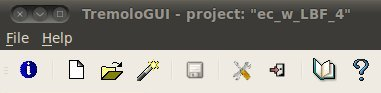
\includegraphics{visuals/GUI_Options.jpg}
\caption{The menu bar in the Tremolo-X GUI. Buttons from left to right:
Project information, new project, open project, creation wizard (not implemented), save project, GUI settings and preferences, GUI exit, GUI help}
\label{GUIoptions}
\end{figure}

\section{\$PROJECTNAME.tremolo} 
\label{.tremolo}
This file could in theory also be named \$ANYTHING.tremolo, with anything deviating from the projectname designated in the file.

\begin{lstlisting}
 global: defaultpath="./$BASENAME";
\end{lstlisting}
The default path is used to allow the use of project independent input files. When the program does not find a specific input file in the current directory, it checks the defaultpath for that file. Since the file may have a basename different from the current project, the basename needs to be specified at all times.

\begin{lstlisting}
global: projectname="$PROJECTNAME";
\end{lstlisting}


Here you actually specify the prefix of all other input files present, which will also be the prefix of the generated output files.
\begin{lstlisting}
global: systemofunits=$SYSTEM_OF_UNITS; 
\end{lstlisting}
This parameter is quite essential as you can choose or customize the system of physical units you wish to use in a particular simulation. The choice made here affects almost any numeric parameter in the simulation and numeric values in other parameter files are expressed in units of the system chosen here.
The options are:
\begin{lstlisting}
 kcalpermole, evolt, si, custom
\end{lstlisting}

\begin{center}
    \begin{tabular}{*{4}{c}}
        \toprule
        {} & kcalpermole & evolt & si \\
        \midrule
        length      & \SI{1}{\angstrom}         & \SI{1}{\angstrom}         & \SI{1}{\meter} \\
        time        & \SI{4.88719e-14}{\second} & \SI{1.01805e-14}{\second} & \SI{1}{\second} \\
        mass        & \SI{1}{\atomicmass}       & \SI{1}{\atomicmass}       & \SI{1}{\kilogram} \\
        current     & \SI{3.27832e-6}{\ampere}  & \SI{1.57377e-5}{\ampere}  & \SI{1}{\ampere} \\
        temperature & \SI{503.556}{\kelvin}     & \SI{11604}{\kelvin}       & \SI{7.2429638e+22}{\kelvin} \\
        \bottomrule
    \end{tabular}
\end{center}
\todo{Check whether the current-unit in kcalpermole is ampere.}

Note, that there is a relation between the scale of the temperature and the energy, which is derived from length, time and mass units. This must be computed individually by the user by dividing the energy by the boltzmann constant.
Below we provide a sample calculation for the eV scaling:
\begin{lstlisting}
# x     sigma = 1 angstrom = 1.e-10 m
# E     u* (sigma/alpha)^2 = epsilon = 1 eV = 1.6021765e-19 kg m^2 / s^2
# t     alpha = 1.0180505e-14 s
# m     u = 1.6605387e-27 kg
# T     epsilon / k_b = 11604.506 K
\end{lstlisting}


\bigbreak

If the choice \texttt{custom} is selected, units must be specified separately according to the following scheme:

\begin{lstlisting}
custom: lengthunit               = {angstrom, nm, m};
custom: lengthscalingfactor      = 1.0;
custom: timeunit                 = {fs, ps, s};
custom: timescalingfactor        = 1.0;
custom: massunit                 = {u, kg};
custom: massscalingfactor        = 1.0;
custom: currentunit              = {"e/s", A};
custom: currentscalingfactor     = 1.0;
custom: temperatureunit          = {K};
custom: temperaturescalingfactor = 1.0;
\end{lstlisting}

By setting any of \texttt{\$PHYSICAL\_QUANTITYscalingfactor} to a value different than $1.0$ all derived physical quantities are affected as well. Thus when using generated output values you need to remember to extract any scaling you introduced here. (Whether you need to divide or multiply, either the factor alone or its square depends on the specific quantity and its units.)


\subsection{Optional input}
\begin{lstlisting}
global: comment="Some comment";
\end{lstlisting}
The comment will be printed to the standard output when the simulation is run.

\subsection{Working with the GUI}
In the GUI this file is controlled by the creation dialog and the first tab. In the creation dialog default path and \$PROJECTNAME must be specified.
\begin{figure}
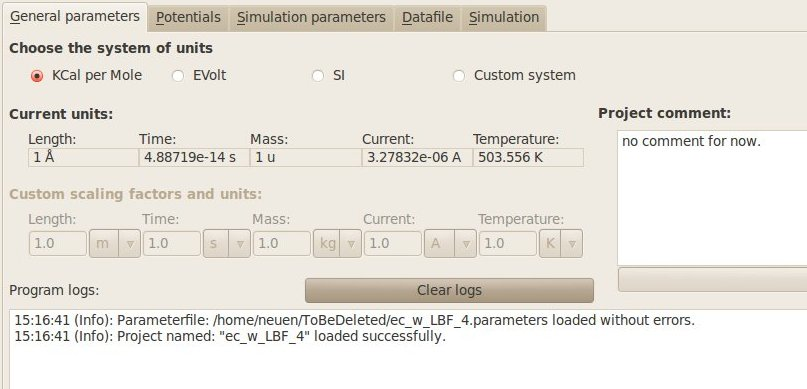
\includegraphics[width=13cm]{visuals/GUI_Main2.jpg}
\caption{}
\end{figure}

\section{\$PROJECTNAME.potentials}
\label{.potentials}
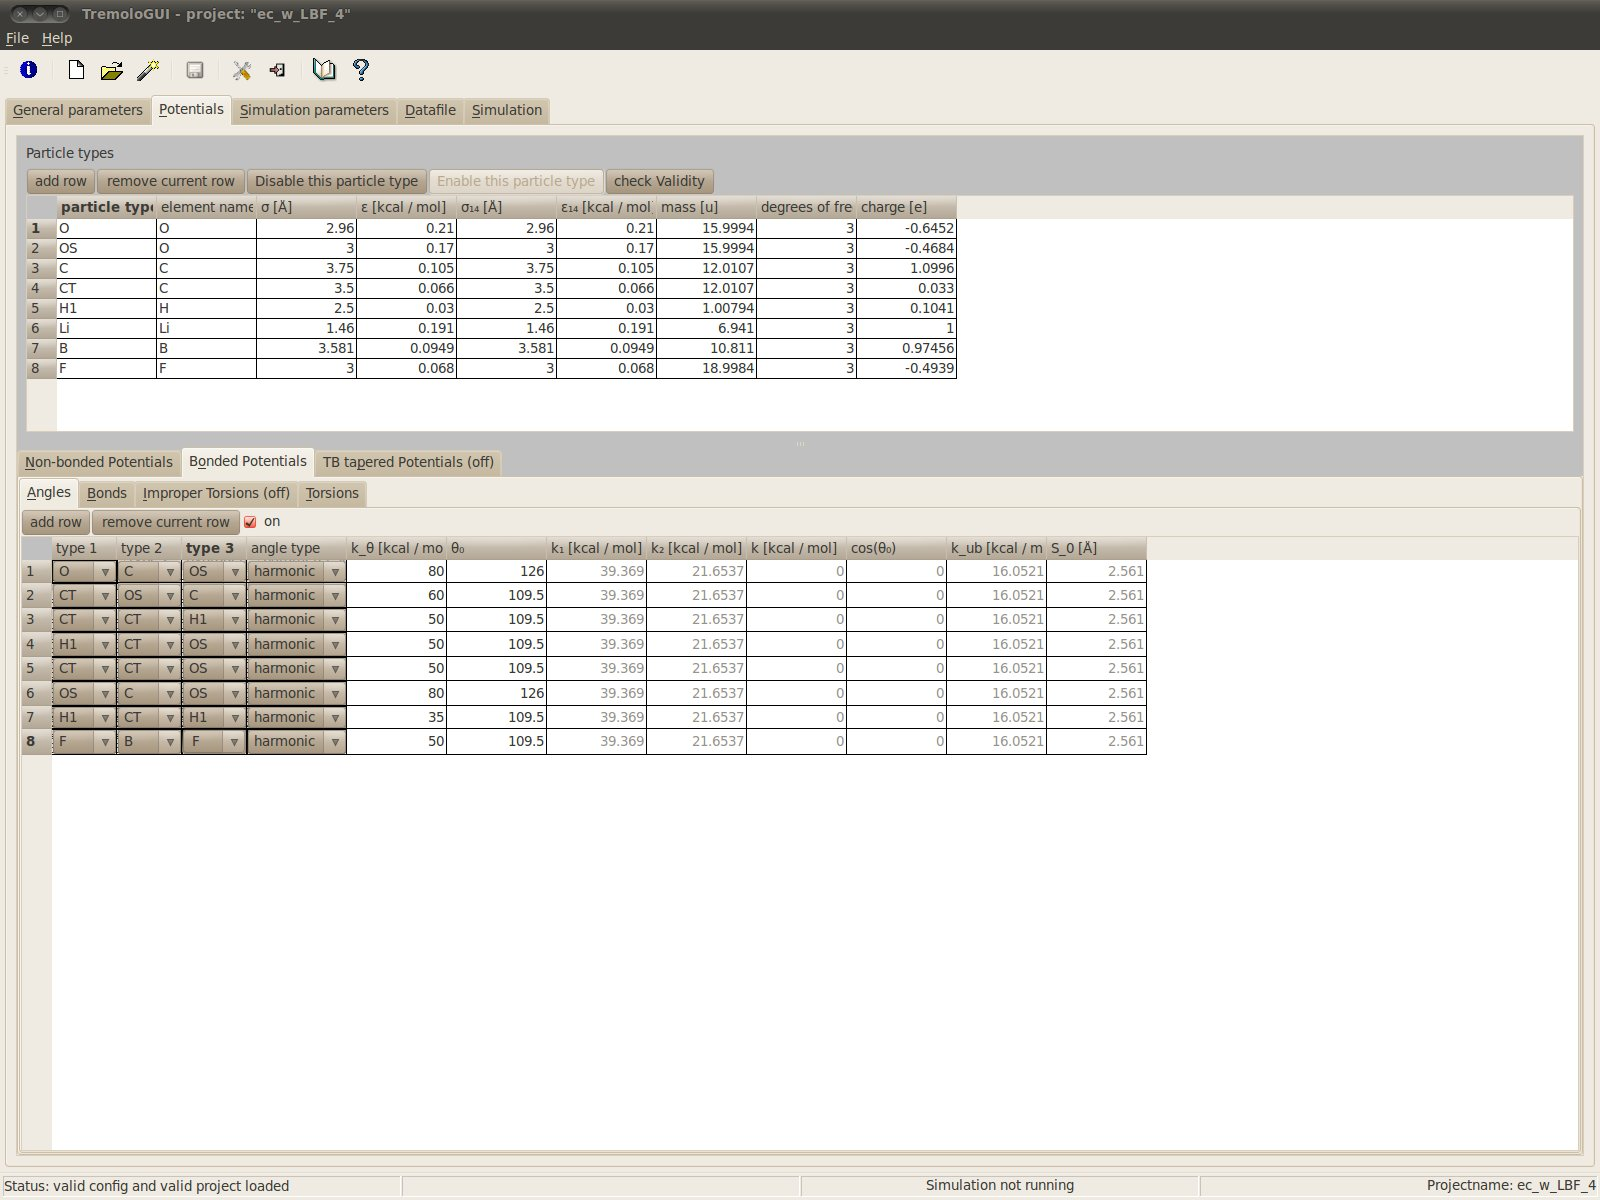
\includegraphics[width=15cm]{visuals/GUI_Potentials_Bonded.jpg}
The potentials file is responsible for all parameters, which affect the forces between atoms in the simulation. It begins with a list of all particle types present in the ensemble, together with some particles which are used more than once: \todo{layout}
{\small
\begin{lstlisting}
 particles	{
 particle: particle_type=$P1, element_name=$NAME1, sigma=1, epsilon=1, sigma14=1, epsilon14=1,    mass=1,    free=3, charge=0;
 particle: particle_type=$P2, element_name=$NAME1, sigma=3, epsilon=1, sigma14=3, epsilon14=0.17, mass=15.9, free=3, charge=-0.4684;
};
\end{lstlisting}
}
The file then lists the potentials, grouped by the type of potential. Each particle requires a specific set of parameters, which, again depending on the type of potential, need to be listed for all pair types (tripled types, ...) of particles to which it shall apply.\todo{layout}
\begin{lstlisting}
nonbonded_2body_potentials      {
   lennardjones:  particle_type1=$P1,  particle_type2=$P1,  r_cut=12.5;
   lennardjones:  particle_type1=$P1,  particle_type2=$P2,  r_cut=12.5;
   lennardjones:  particle_type1=$P2,  particle_type2=$P2,  r_cut=12.5;
   ljspline:      particle_type1=$P1,  particle_type2=$P1,  r_cut=12.5,  r_l=11;
   ljspline:      particle_type1=$P1,  particle_type2=$P2,  r_cut=12.5,  r_l=11;
   ljspline:      particle_type1=$P2,  particle_type2=$P2,  r_cut=12.5,  r_l=11;
        };
\end{lstlisting}

\todo{Make entry for each potential.}

\section{\$PROJECTNAME.validates}
\label{.validates}

All particles and force fields detailed in the .potentials file need to be validated in this file, by setting their state to on. The reason for this is the converse action, this allows to selectively deactivate particle types and force fields, which shall not be used in this particular situation. This might be relevant, if you wish to experiment with several different (combinations of) force fields: Instead of writing an entire .potentials file for each combination, one such file with all desired forcefields is sufficient and you only need to make minor changes to the .validates file.

\begin{lstlisting}
validate: particle_type=$P1, state=on;
validate: particle_type=$P2, state=off;

validate: force_type=lennardjones, state=off;
validate: force_type=ljspline, state=on;
\end{lstlisting}


\section{\$PROJECTNAME.data}
\label{.data}
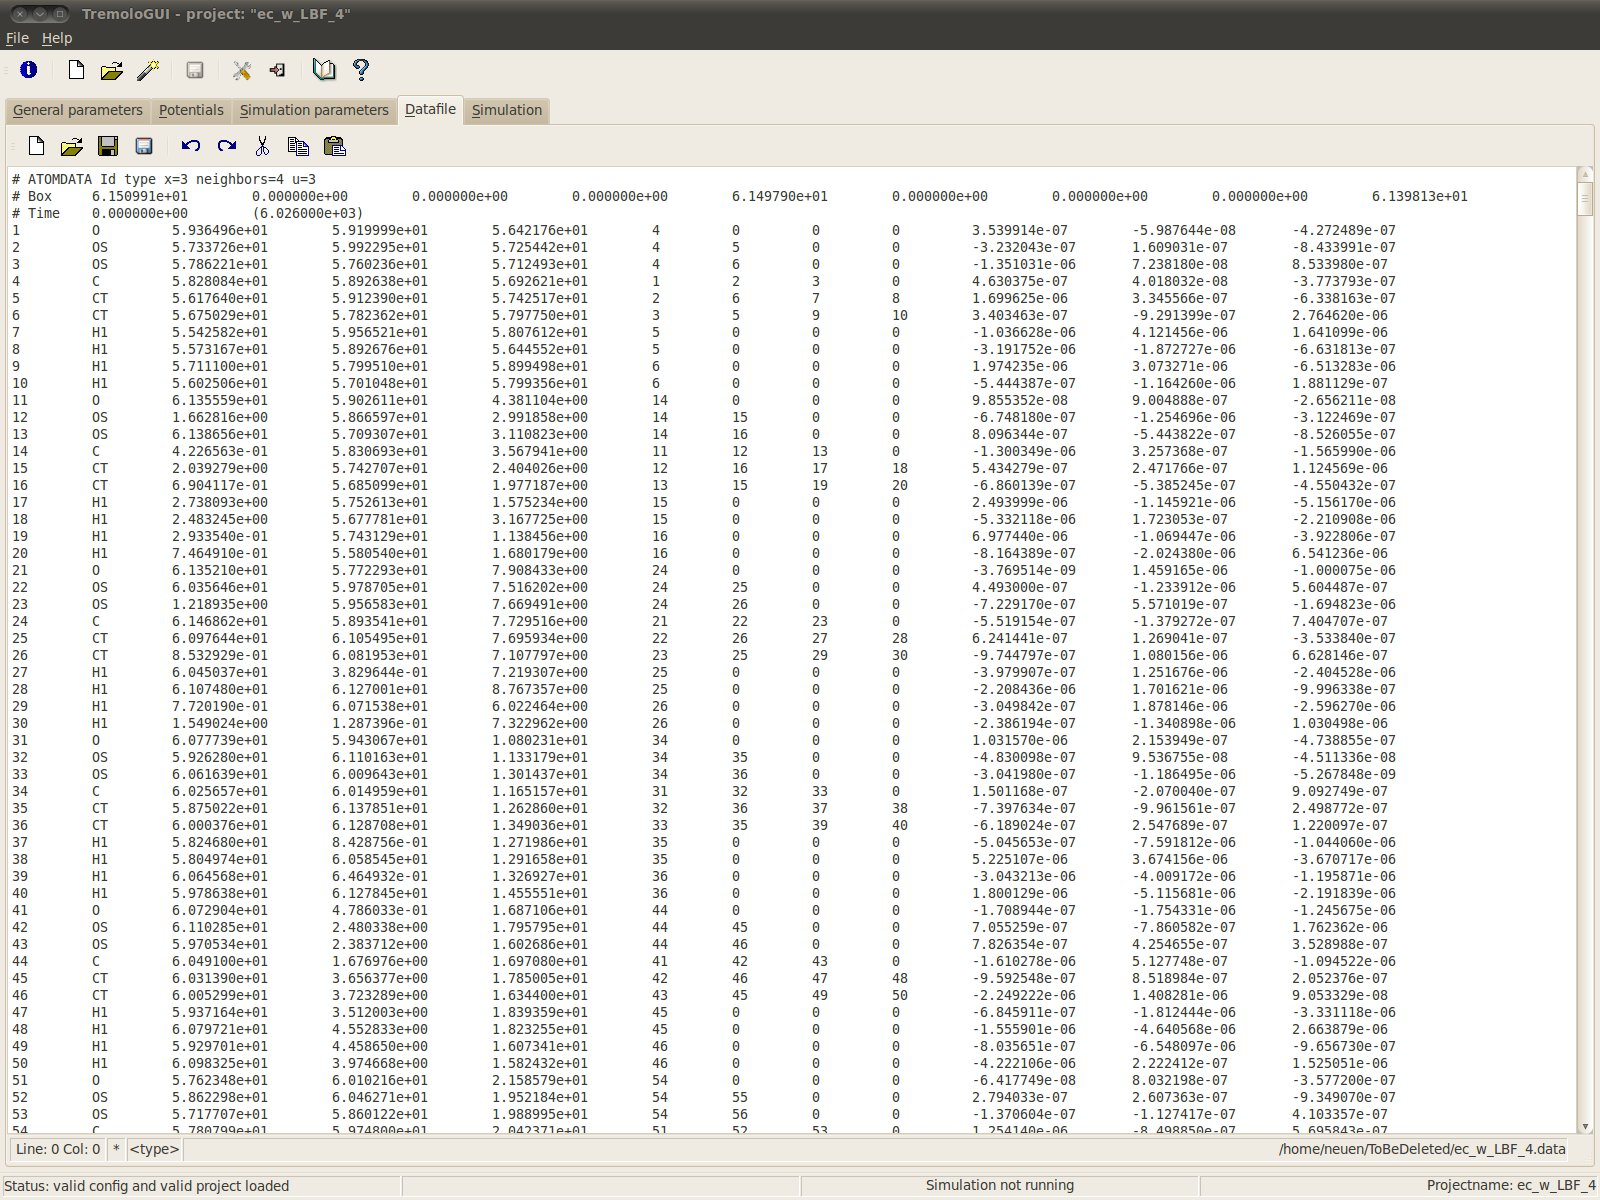
\includegraphics[width=15cm]{visuals/GUI_Data.jpg}

This file contains all information about the initial configuration of the atoms. Always present is the line \texttt{ATOMDATA} line, which informs the parser about the type and order of the input. It may be followed by some optional \texttt{ATOMDATAADDOUT}, \texttt{INPUTCONV} and \texttt{OUTPUTCONV} lines.
\begin{lstlisting}
ATOMDATA  <record_entry_1> ... <record_entry_n>
 <record_entry>: <dataname>[=<n>]
 <dataname>    : x | xs | u | F | stress | Id | charge | GroupMeasureTypeNo | type | neighbors | extType | imprData | name | resName | chainID | resSeq | occupancy | tempFactor | segID | Charge
               
\end{lstlisting}



In the example below the line specifies the options \texttt{Id} and \texttt{type}, which occupy a single column each. This is followed by the particle positions \texttt{x}, which require a three column wide vector, neighbors with a four column vector and finally velocities \texttt{u}, which use three columns again. Note that all options are case sensitive.\todo{layout}
{\tiny
\begin{lstlisting}
# ATOMDATA Id type x=3 neighbors=4 u=3
1       O       5.936075e+01    5.915340e+01    5.643238e+01    4       0       0       0       3.540887e-07    -5.986875e-08   -4.272449e-07   
2       OS      5.734245e+01    5.991388e+01    5.725724e+01    4       5       0       0       -3.232931e-07   1.608824e-07    -8.433911e-07   
3       OS      5.782428e+01    5.758512e+01    5.712316e+01    4       6       0       0       -1.351403e-06   7.237250e-08    8.533900e-07    
4       C       5.826889e+01    5.890171e+01    5.693151e+01    1       2       3       0       4.631648e-07    4.017515e-08    -3.773758e-07  
\end{lstlisting}
}
Possible options and their meaning are:
\begin{itemize}
\item \texttt{type} (string) This parameter must be present and it must match one of the particle types specified in the .potentials file.

\item \texttt{Id} An identifier for each particle. When this parameter is used id numbers need to be assigned sequentially, 
  otherwise there may be unexpected behavior. This is a requirement for the use of \texttt{neighbors}.

\item {\tt x=3} This are the carrtesian coordinates. The only sensible vector length is three.

\item {\tt xs=3} This are the scaled/fractional coordinates. The only sensible vector length is three. Note that {\tt x=3} or {\tt xs=3} must be given.

\item {\tt u=3} If one wishes to give particular velocities to individual particles, this can be specified here. In the case of a dynamics simulation it is set by default for the data output files. This way, you are able to restart the simulation from the finishing point. 
  Supplying starting velocities also fixes an initial temperature and may conflict with the corresponding option 
  \ref{INPUTCONV}, which takes precedence. The only sensible vector length is three.

\item {\tt neighbors=<n>} This parameter(-vector) specifies the particles to which the present one is bonded by specifying 
  its {\tt Id} number. The identifier {\tt Id} numbers must exist and a particle may not be linked to itself. For non-bonds, 
  enter a zero instead. The length of this vector can be any positive integer. This is relevant for bonded force fields.

\item {\tt charge} This parameter fixes an (electric) charge for this parameter. To have an effect, some Coulomb 
  potential must be used. (This overwrites the charge set in the .potentials file for the particle type \todo{test whether this is correct.}

\item {\tt F=3} This option allows to write out the current forces on each particle at the output time step.
  \todo{It is advised to start with zero entries in these columns. The necessity should be verified.}

\item {\tt stress=<n>} This allows the output of this particles contribution to the total box stress. 
  While not a physical stress value by itself (point particles do not have stress) this allows to determine 
  local stress in a macro-structure by comparison among the particles. In the case you set the option in the parameter file to measure the local stress, it is set by default for the data output files.

\item {\tt imprData=<n>} When using improper torsion forces, use this as {\tt neighbors} in order to specify 
  neighbors for the respective force.

\item {\tt GrpTypeNo} For certain measurement routines, particles may be assigned to groups, which do not need 
  to respect particle types. \todo{specify relevant options, 4 indices?}
\end{itemize}
The information below belongs to PDB information, they are only parsed in and written out, they have no effect on simulation
\begin{itemize}
\item {\tt extType} type number used for external forces \todo{Is this actually a PDB option?}
\item {\tt name} particle name (used only for PDB data)
\item {\tt resName} residue name (used only for PDB data)
\item {\tt chainID} chain ID (used only for PDB data)
\item {\tt resSeq} residues sequence number (used only for PDB data)
\item {\tt occupancy} occupancy (used only for PDB data)
\item {\tt tempFactor} temperature factor (used only for PDB data)
\item {\tt segID} segment ID (used only for PDB data)
\item {\tt Charge} Charge (string) (used only for PDB data)
\end{itemize}
For the proper handling of PDB parameters, this feature must have been enabled at configure time of Tremolo-X. \todo{Discuss enable by default.}

You can use an ATOMDATAADDOUT line in the same way to output additional data in the data output files, e.g. to write out forces in the above example:
 \begin{lstlisting}
# ATOMDATA Id type x=3 neighbors=4 u=3
# ATOMDATAADDOUT F=3
\end{lstlisting}

Note that one can also give the box matrix by a \texttt{\# BOX} line
in the \texttt{.data} file. In particular, a \texttt{\# BOX} line
given in the \texttt{.data} file will overwrite values from the
\texttt{.parameter} file.
\begin{lstlisting}
# BOX xx xy xz yx yy yz zx zy zz
\end{lstlisting}

\subsection{Input conversion}
\label{INPUTCONV}
The .data file may contain options, which influence the starting configuration of the sample. In the following list, {\tt \{0|1\} } indicates that the option is activated by setting the integer to 1, while it is deactivated with 0. The default behavior (on/off) depends on the option and is listed.
\begin{itemize}

\item {\tt \# INPUTCONV shift} Shift of initial particle coordinates by specifying a vector or by positioning the {\tt (0. 0. 0.)} 
  coordinate in the center of the simulation domain (this would be equivalent to the half of the diagonal vector of the simulation domain.) 
  Either supply vector {\tt x y z} or write {\tt center}. Note that the shift vector is given in scaled/fractional coordinates, e.g.\ the center is  {\tt (0.5 0.5 0.5)}.
\item {\tt \# INPUTCONV trans} Transformation of initial particle coordinates by a matrix {\tt A} (which needs to be supplied as: 
  {\tt <A\_xx> <A\_xy> <A\_xz>  <A\_yx> <A\_yy> <A\_yz>  <A\_zx> <A\_zy> <A\_zz>}) Transformation is done after shifting. Note that the transformation is applied on scaled/fractional coordinates.
\item {\tt \# INPUTCONV periodic 1|0} Enable/Disable periodic correction for coordinates of inserted particles.
  This feature is active by default.
\item {\tt \# INPUTCONV temp \#FLOAT} is specified all particles are assigned a Maxwell-Boltzmann distributed velocity, 
  such that the total kinetic energy corresponds to the temperature value specified (in units of the chosen system. 
  Using this option overwrites any user specified velocities. Note that the kinetic energy will most likely change over 
  the course of the simulation, unless a thermostat is in use.
\item {\tt \# INPUTCONV moment 0|1} results in the computation of the total momentum and a correction of all particle velocities,
  such that the new momentum is zero at the start of the simulation. Note that the use of a thermostat, 
  while maintaining the kinetic energy might cause the momentum to change over the course of the simulation runtime. 
  (On the momentum conservation of thermostats, see section \ref{thermostats}) This feature is inactive by default.
\item {\tt \# INPUTCONV angmoment 0|1} results in the computation of the total angular momentum and a correction of all particle velocities, 
  such that the new angular momentum is zero at the start of the simulation. Note that the use of a thermostat, 
  while maintaining the kinetic energy might (will most likely) cause the angular momentum to change over the course of the simulation runtime. This feature is inactive by default.
\end{itemize}
Note that \# is always part of the command. Thus, comments may not be added to this file, as they would interfere with the parsing of the regular commands.


If both momentum correction and temperature distribution are set, then first the
temperature distribution is set, then the moment is corrected, then the velocities
are scaled again to match the temperature.

 Example file:
\# ATOMDATA x=3 type
\# INPUTCONV shift center
\# INPUTCONV temp 0.57
\# INPUTCONV moment 1
\# INPUTCONV angmoment 1
0 0 0 C
0 1 0 H
0 0 1 H
\subsection{Output conversion}
\label{OUTPUTCONV}


\section{\$PROJECTNAME.parameters}
\label{.parameters}

This file contains the most extensive set of options, which may also interfere with each other. Therefore, this section only serves to explain the syntax of the file, while the comprehensive explanation of the option is moved to the following chapters.

The basic syntax scheme is the following:
\begin{lstlisting}
$ITEM1: $PARAMETER1=#VALUE, $PARAMETER2=#values;
$ITEM2: $PARAMETER1=#VALUE;
$CATEGORY {
       $ITEM1: $PARAMETER1=#VALUE;
       $ITEM2: $PARAMETER1=#VALUE, $PARAMETER2=#values, ... ;
       $SUBCATEGORY  {
                $ITEM1: $PARAMETER1=#VALUE;
                $ITEM2: $PARAMETER1=#VALUE, $PARAMETER2=#values, ... ;
                $ITEM3: $PARAMETER1=#VALUE, $PARAMETER2=#values;
                  };
            };
};
\end{lstlisting}
Modifications from this scheme occur for the propagator and timelines\fixme{Timelines working?} and are described there in detail.



With two exceptions the parameters are grouped into the following categories:
\begin{itemize}
 \item domain \ref{sub:domain}, \ref{domain}
 \item optimization \ref{sub:optimization}, \ref{optimization}
 \item dynamics \ref{sub:dynamics}, \ref{ensembles}
 \item coulomb \ref{sub:coulomb}, \ref{longrange}
 \item parallelization \ref{sub:parallelization}, \ref{parallelization}
 \item output \ref{sub:output}, \ref{measurement}
\end{itemize}

There are two parameters, which are not associated with any of the above categories. The basic choice, whether the simulation type should be optimization or dynamics, determines, whether the parser takes options from the dynamics section or from the optimization section:
\begin{lstlisting}
 integration: type=$TYPE;
\end{lstlisting}
where \$TYPE = \{\textit{dynamics, optimization}\}.
\bigbreak
The other stand alone parameter is the cut``radius'' of the linked cells, which is set by
\begin{lstlisting}
 lcs:    cellrcut=#FLOAT;
\end{lstlisting}
where \#FLOAT is a positive floating point number. Also, the \texttt{cellrcut} must be smaller than the box dimensions or in case of parallel computations smaller than the box length divided by the number of processes in each direction.

Example: Your domain is 15x15x16. If you employ 3x3x3 processes, your \texttt{cellrcut} may not exceed 5. If you employ 3x3x4 processes your \texttt{cellrcut} may not exceed 4.

It is sensible to choose the \texttt{cellrcut} just as small, that cut off radii of pair potentials just fit into one cell~\cite{GriebelEng}.

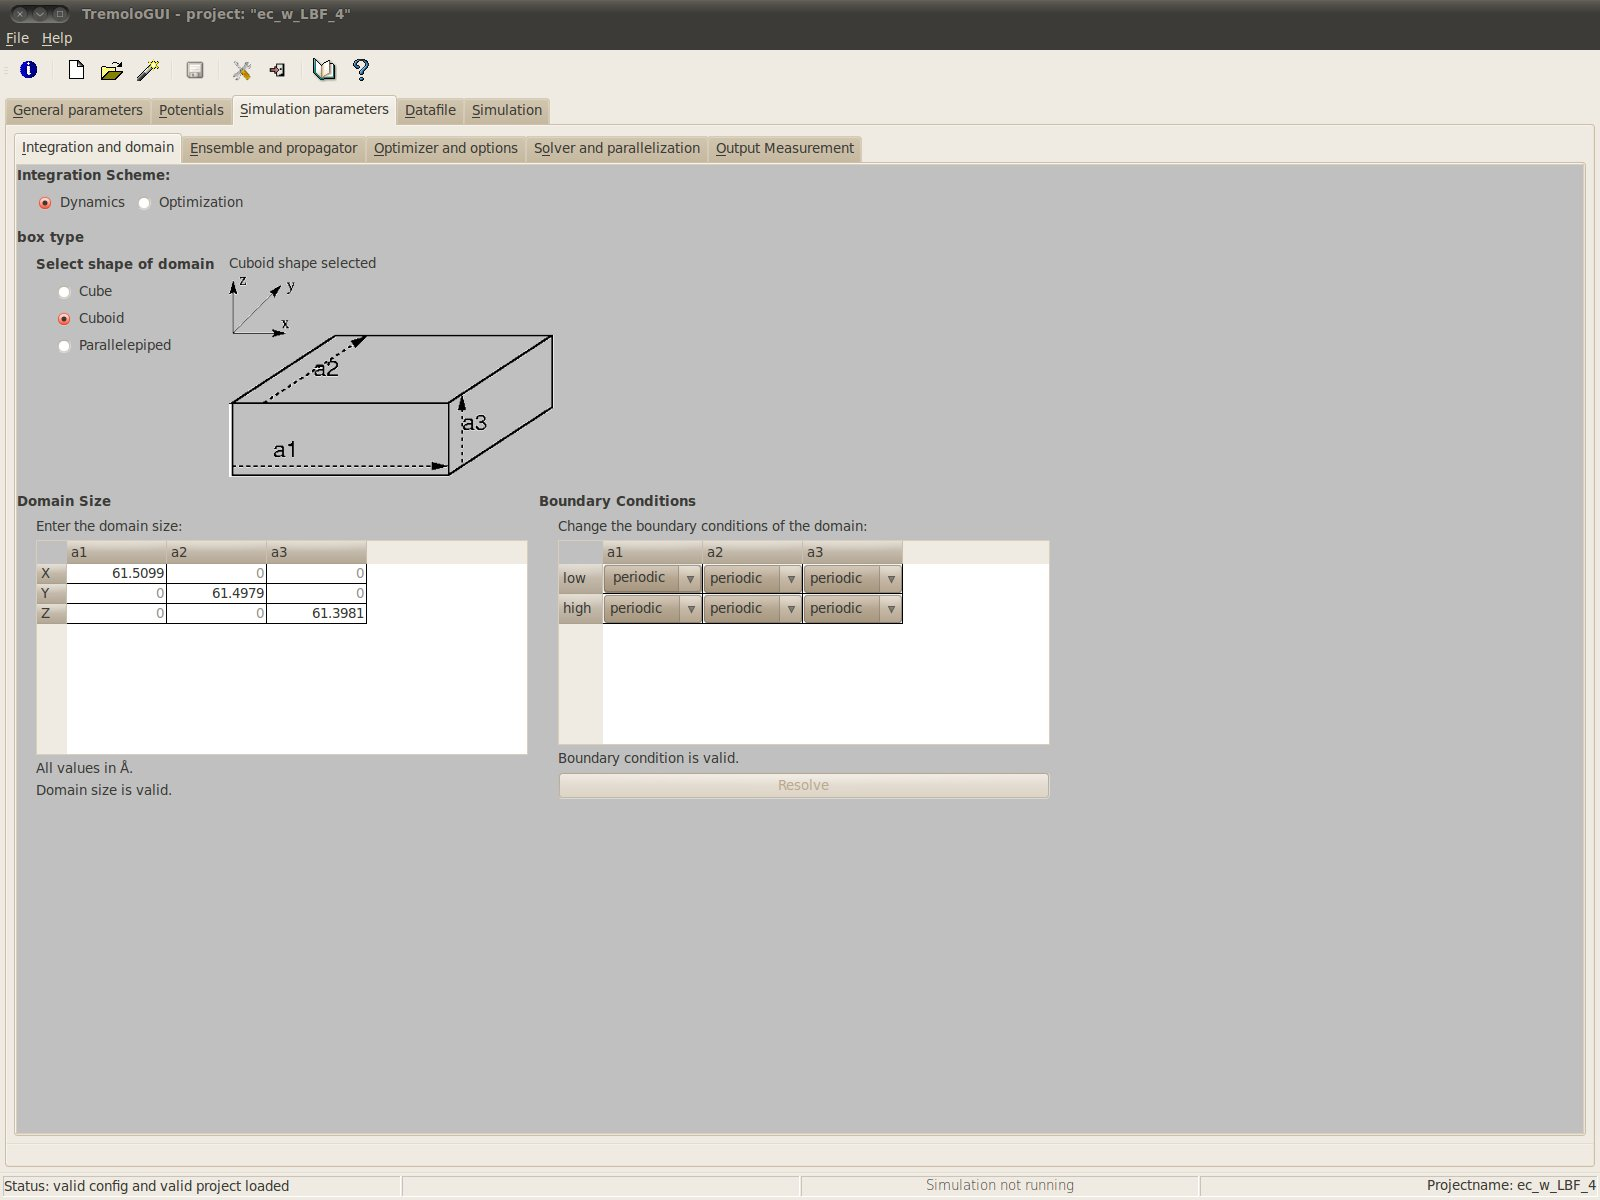
\includegraphics[width=15cm]{visuals/GUI_Parameter_Integration_Domain.jpg}
\subsection{domain}
\label{sub:domain}

The category domain contains the items:
\begin{lstlisting}
size:
type     = {cube, diag, matrix},
size     = #FLOAT,
length_x = #FLOAT, length_y = #FLOAT, length_z = #FLOAT,
xx = #FLOAT, xy = #FLOAT, xz = #FLOAT,
yx = #FLOAT, yy = #FLOAT, yz = #FLOAT,
yx = #FLOAT, zy = #FLOAT, zz = #FLOAT;
\end{lstlisting}

Depending on the type specified, you may leave out the size entries for the other categories, e.g. 
\begin{itemize}
 \item for {\tt cube} you only need to specify \texttt{size}, which is a uniform edge length,
 \item for {\tt diag} you need to set \texttt{length\_x, length\_y and length\_z},
 \item for matrix you need to set the edge vector in the matrix (There are vectors x,y,z with components x, y, z.).
\end{itemize}
The other specifiers may be omitted, however if you supply them the programm will ignore them safely.

Note that one can also give the box matrix by a \texttt{\# BOX} line
in the \texttt{.data} file. In particular, a \texttt{\# BOX} line
given in the \texttt{.data} file will overwrite values from the
\texttt{.parameter} file.
\begin{lstlisting}
# BOX xx xy xz yx yy yz zx zy zz
\end{lstlisting}

\begin{lstlisting}
border:
bt_xlow  = {periodic, leaving, reflecting},
bt_xhigh = {periodic, leaving, reflecting},
bt_ylow  = {periodic, leaving, reflecting},
bt_yhigh = {periodic, leaving, reflecting},
bt_zlow  = {periodic, leaving, reflecting},
bt_zhigh = {periodic, leaving, reflecting};
\end{lstlisting}

The options {\tt leaving} and {\tt reflecting} may be mixed, whereas {\tt periodic} must always match for the respective low and high borders.

\subsection{dynamics}
\label{sub:dynamics}
we have the items:
\begin{lstlisting}
ensemble:       ensemble={NVE, NVT, NPT, NPE};
\end{lstlisting}
\begin{lstlisting}
propagator,     $INTEGRATOR: delta_T=#FLOAT,  endtime=#FLOAT,     timeinteps=#FLOAT,       maxiteration=#INTEGER;
\end{lstlisting}
%$

\$INTEGRATOR = \{{\tt verlet, beeman2, beeman3, beeman4, beeman5, beeman2v, beeman3v}\}

The parameters \texttt{timeinteps} and \texttt{maxiteration} are only relevant in the case of an velocity type algorithm, they are used for aborting the iteration procedure, either when the iterative error drops below \texttt{timeinteps} or the number of iteration cycles reaches \texttt{maxiteration}.

\subsubsection{thermostat}
The subcategory \textbf{thermostat}
%\begin{lstlisting}nose:   	    state={on, off},      F_Mass=#FLOAT;\end{lstlisting}
\begin{lstlisting} nosehoover:         state={on, off},      F_Mass=#FLOAT; 
\end{lstlisting}
\begin{lstlisting}
berendsen:          state={on, off},      T_Interval=#FLOAT;
\end{lstlisting}
%\begin{lstlisting}dpd:    	    state={on, off},      gamma=#FLOAT,        r\cut=#FLOAT;\end{lstlisting}
\begin{lstlisting} constanttargettemp: state={on, off},      T_Temp=#FLOAT;
\end{lstlisting}
%\begin{lstlisting}timeline:          state={on, off},      [time,  temperature,    interpolation=(0,     0,      constant)];\end{lstlisting}
\todo{nose, dpd, timeline (working?)}

\subsubsection{barostat}                   
The subcategory \textbf{barostat}
{\small
\begin{lstlisting}
parinello: state={on, off},      f_mass=#FLOAT;
constraint: type={isotropic, standard, symmetric, none};
constraintmap: xx={0|1}, xy={0|1}, xz={0|1}, yx={0|1}, yy={0|1}, yz={0|1}, zx={0|1}, zy={0|1}, zz={0|1};
constantpressure: state={on, off},       Pressure=#FLOAT;
Timeline: state={on, off},      [time,  pressure,  interpolation=(0, 0, constant)];
stresstensor: [time,  stress, interpolation, xx, xy, xz, yy, yz,zz=(0, 0, constant, 0, 0, 0, 0, 0, 0)];
\end{lstlisting}
}

For theoretical background and detailed description of the options see section \ref{section:ensembles:barostat}.
The first option obviously switches the barostat on/off. The second option determines the virtual mass
assigned to the box.
In the constraint line one of the four constraint types must be chosen, which will work together with the 
following selection from the constraintmap.
The selection of the constraintmap must always obey symmetry and in the isotropic case the ``1'' entries
must be restricted to the diagonal. It is possible to 


\todo{constraintmap, stresstensor; timeline(working?)}

When a constraint type is chosen, this places certain restrictions on the constraintmap, however the user still needs to set it accordingly. 
(The constraintmap is not locked, since it allows the user to enforce restrictions to subdimensions.)
The constraintmap must always observe \texttt{xy=yx} etc., even for the non symmetric restrictions.
\begin{itemize}
\item The \texttt{isotropic} constraint allows only changes on the main (diagonal) axis. Furthermore those changes are enforced to be isotropic, meaning the changes are identical in all allowed directions. (e.g. the user may set only \texttt{xx} and \texttt{yy} to 1, prohibiting changing of the box in the z direction.)
\item \texttt{standard} the box deformation is restricted to an upper triangular matrix.
\item \texttt{symmetric} constraints enforce symmetry in the box deformation. 
\item \texttt{none} No additional constraints are placed on the deformation tensor. Note that this is unphysical.
\end{itemize}

In the following lines we can specify the mean pressure applied to the system (both as a constant and as a timeline), as well as a stresstensor, 
which is externally applied, independent of the stress exerted by the particles in the system.

\subsection{optimization}
\label{sub:optimization}
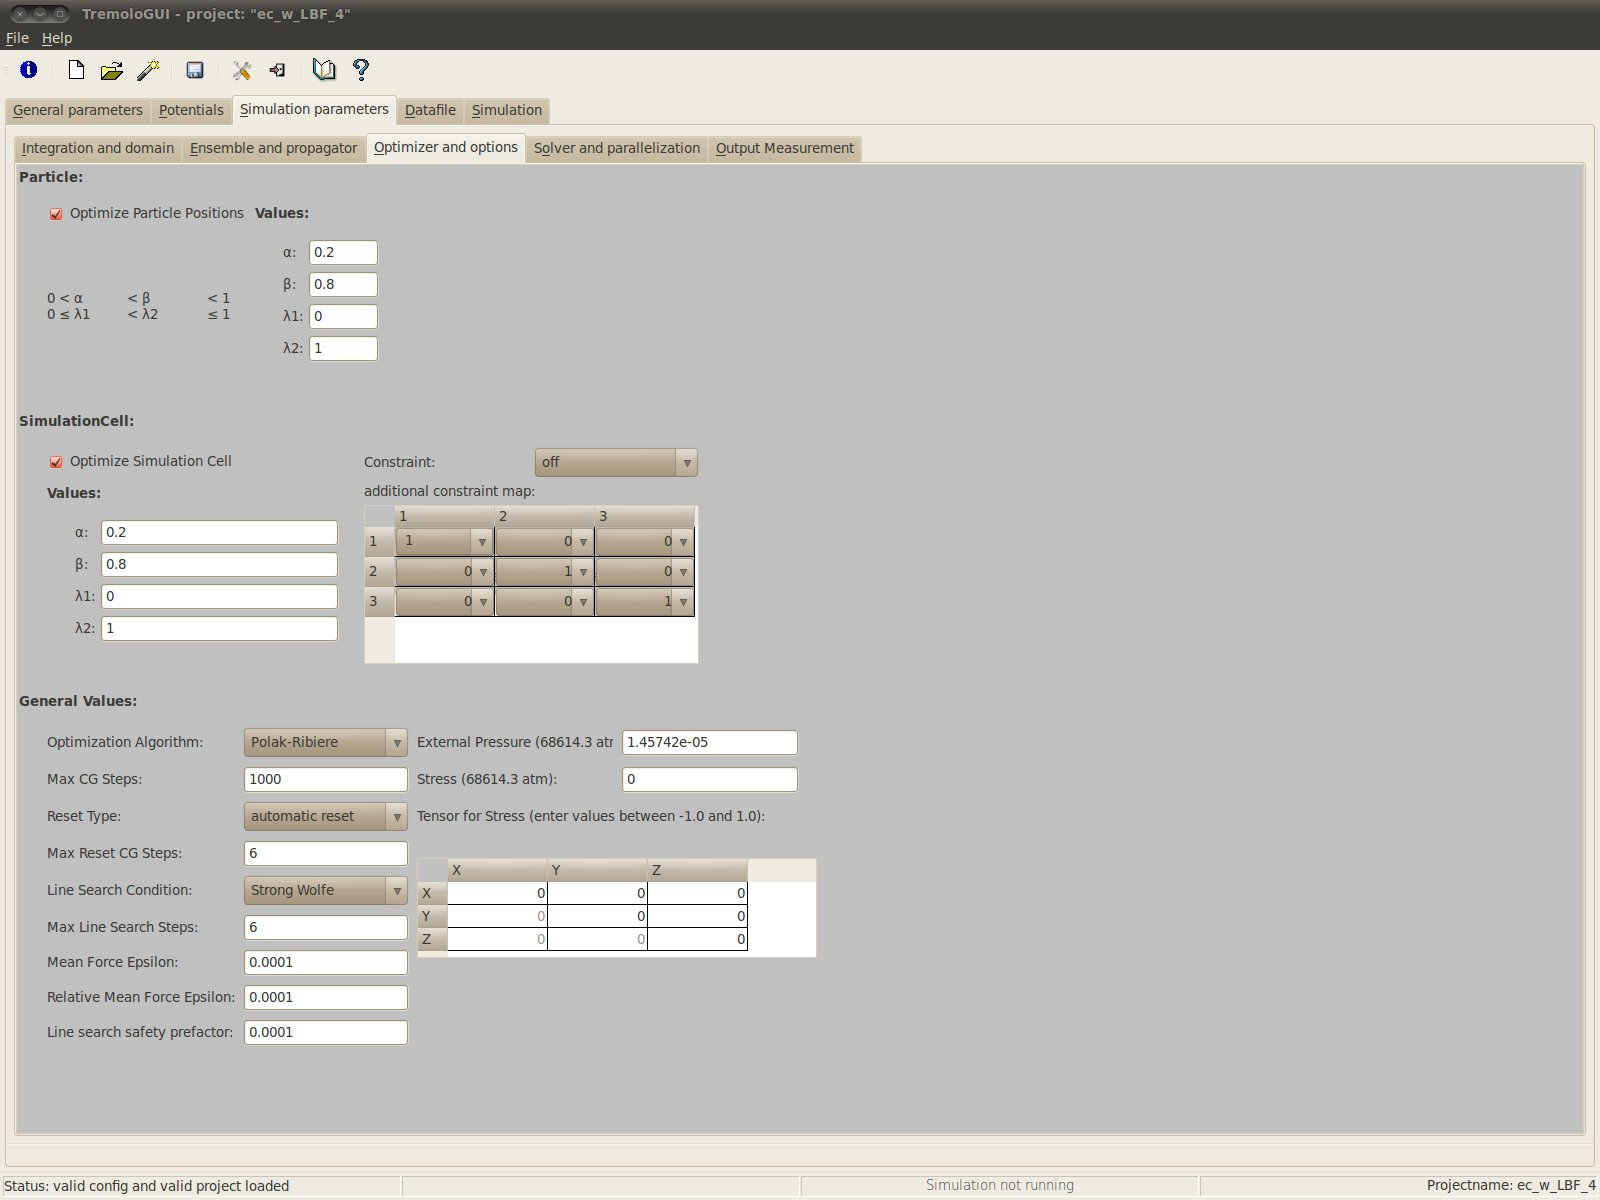
\includegraphics[width=15cm]{visuals/GUI_Parameter_Optimizer.jpg}

\begin{lstlisting}
optimization{
  particle: state=on,  alpha=0.2,   beta=0.8,    lambda1=0,   lambda2=1;
  simucell: state=off, alpha=0.2,   beta=0.8,    lambda1=0,   lambda2=1;
  simucell: constraint=isotropic,  XX=1,  XY=0,  XZ=0,  YX=0,  YY=1,  YZ=0,  ZX=0,  ZY=0,  ZZ=1;
  common:   algorithm=fr,  maxcg=102,  RT=periodical,  maxresetcg=6,  LS=wolfe,   maxlinesearch=6,   mean_force_eps=1e-05,  mean_force_eps_rel=1e-05,  prefactor=0.001, extpressure=1;
  stress:   stress=0,  XX=0,  XY=0,  XZ=0,  YX=0,  YY=0,  YZ=0,  ZX=0,  ZY=0,  ZZ=0;
};
\end{lstlisting}

\todo{complete optimization}
\subsection{coulomb}
\label{sub:coulomb}
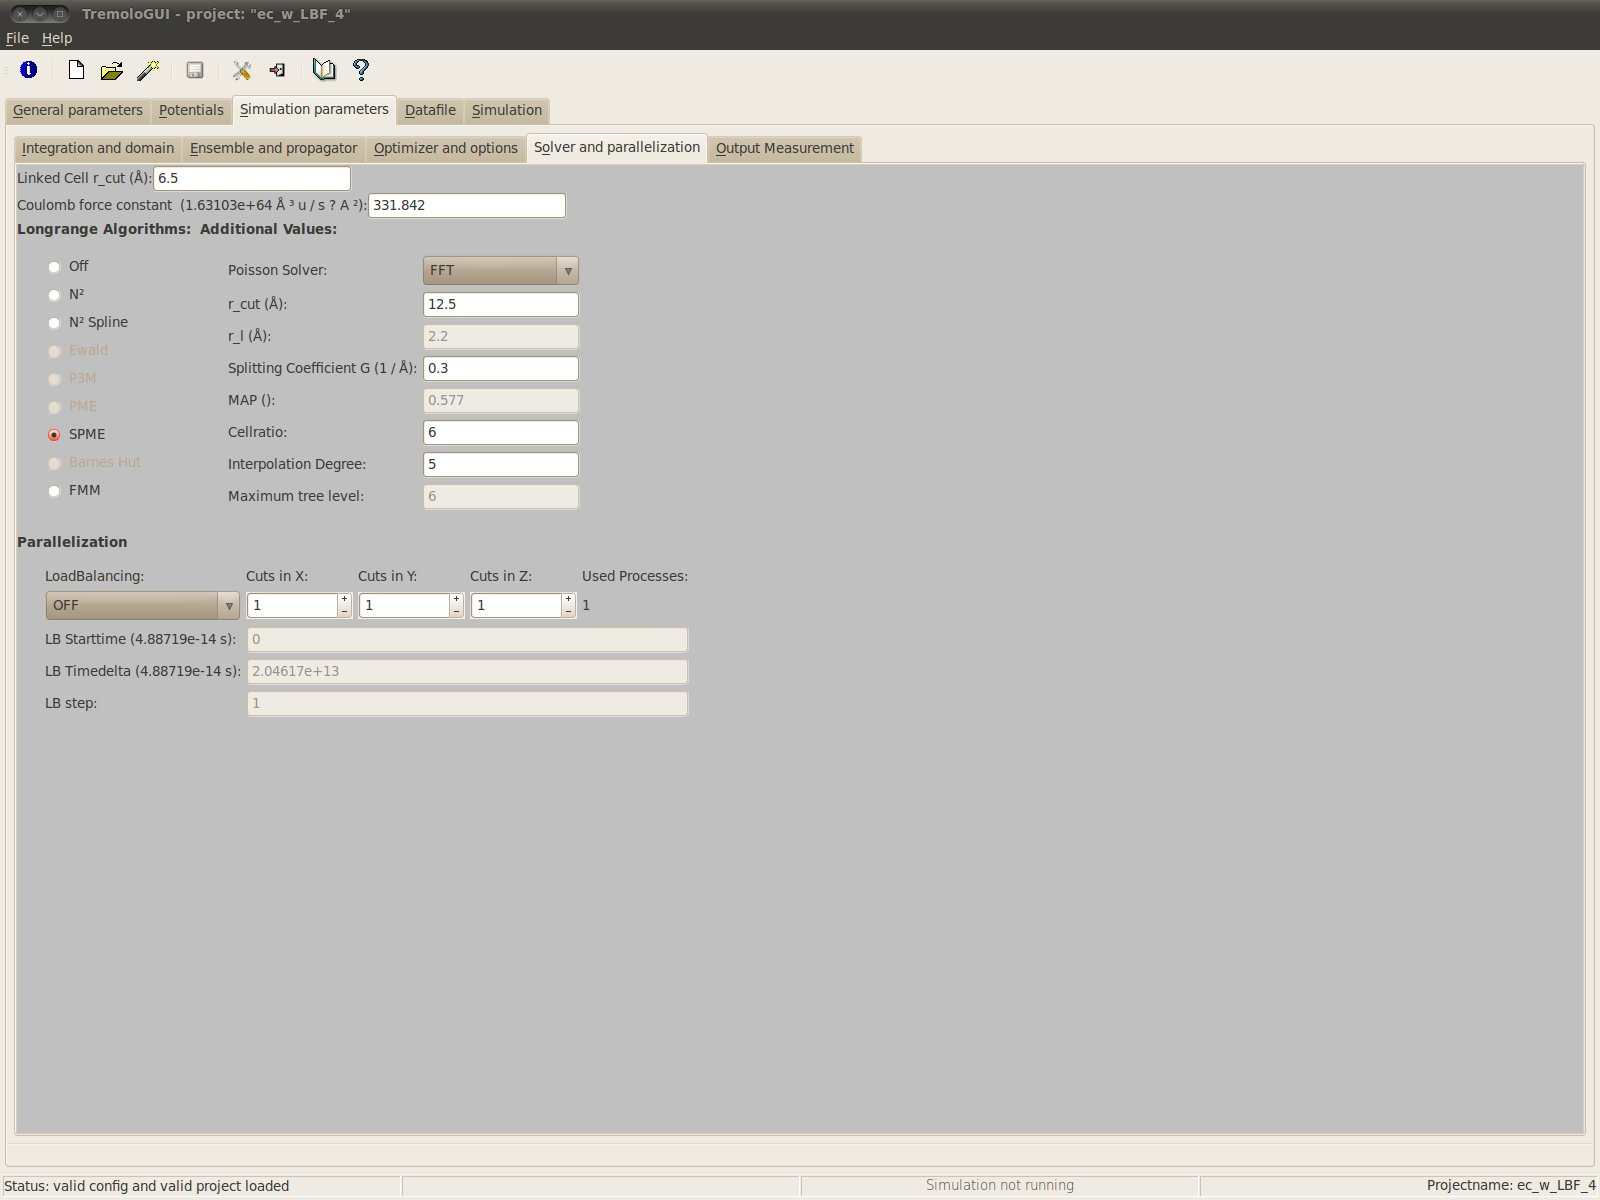
\includegraphics[width=15cm]{visuals/GUI_Parameter_LongRange_Parallel.jpg}
\begin{lstlisting}
coulomb {
permittivity:   epsilon0inv=1.9620959e-21; 
n2:        state=off, r_cut=0.7352941, i_degree=5;
n2spline:  state=off, r_cut=0.7352941, r_l=0.6470588, i_degree=5;
ewald:     state=off, r_cut=0.7352941, G=1.19e-10,    i_degree=5,  cellratio=6;
p3m:       state=off, r_cut=0.7352941, G=1.19e-10,    i_degree=5,  cellratio=6,  ps=fft;
pme:       state=off, r_cut=0.7352941, G=1.19e-10,    i_degree=5,  cellratio=6,  ps=fft;
spme:      state=off, r_cut=0.7352941, G=1.19e-10,    i_degree=5,  cellratio=6,  ps=fft;
barneshut: state=off, r_cut=0.7352941, mtl=6,         i_degree=5;
fmm:       state=off, r_cut=0.7352941, mtl=6,         i_degree=5,  Map=0.577;
};
\end{lstlisting}

Currently \texttt{n2}, \texttt{n2spline} and \texttt{spme} are implemented.

\emph{Note that the \texttt{SPME} method
is not implemented sequentially and requires a Tremolo-X version with parallel capabilities. 
You can start the parallel version with one process though and use SPME nevertheless.}
\subsubsection{Permittivity}
The coulomb-force-constant epsilon0inv is the only constant which is truly associated with units.
(All others are converted to a reduced state.) As such it is dependent on the choice of the unit system. 
In this context it is necessary to note, that there are several different definitions of the calory,
which need to be distinguished.
Despite its name it is not the inverse of $\epsilon_0$.
\begin{equation*}
\text{\tt epsilon0inv}=\frac{1}{4 \pi \epsilon_0} \cdot \frac{e^2}{\left[length\right],}
\end{equation*}
where $e$ is the respective charge unit and $\left[length\right]$ the unit of length used.

A few common examples, which all use the electron charge and angstrom but convert to different reference energies, are:
\begin{itemize} 
\item Using angstrom and kcal$_{th}$/mol:\\
$ \frac{1}{4*\pi*\epsilon_0} * (e^2/angstrom) = 332.06371 \quad kilo cal_{th} / mol N_A$

\item Using angstrom and kcal/mol:\\
$ \frac{1}{4*\pi*\epsilon_0} * (e^2/angstrom) = 331.84164  \quad kcal_{mol}$

\item Using angstrom and eV:\\
$ \frac{1}{4*\pi*\epsilon_0} * (e^2/angstrom) = 14.399644  \quad eV $
\end{itemize}

\subsubsection{r\_cut, r\_l}
The r\_cut parameter determines the separation of short and long range part of the potential. For the case of the splined N$^2$-Algorithm 
r\_l defines the radius from which spline interpolation to the cut-off starts. For more information see section \ref{longrange}.
\subsubsection{i\_degree}
This parameter determines the degree of the polynomials used for the field interpolation.
\subsubsection{G}
Localization parameter for the smooth screening functions. With larger G the localization is tighter.
\todo{Suggest to keep values between 0.24 and 0.35 1/angstrom?}
\subsubsection{cellratio}
Ratio of interpolation nodes per LC cell in one dimension. (Depending on the method this may be enlarged to the next power of two.)
\subsubsection{mtl}
Maximal tree level of the multipole method.

\todo{complete coulomb}


\subsection{parallelization}
\label{sub:parallelization}
Parameters for domain decomposition can be set on the command line when calling the program. If this is done, those parameters supersede and replace those set in the 
{\tt .parameters} file.

\begin{lstlisting}
parallelization {
    proc:     n1=1,   n2=1,   n3=1,   all=1;
    loadbal:  wf=off, Lb\_t=0, Lb\_delta=4.608295e+11,  Lb\_step=1;
};
\end{lstlisting}
\subsubsection{Number of processors}
The numbers {\tt n1}, {\tt n2} and {\tt n3} are the number of cell bins per respective dimension. Their product must equal the total number of processes assigned with {\tt all}.
\subsubsection{Loadbalancing}

\todo{complete parallelization}
\subsection{output}
\label{sub:output}
\begin{lstlisting}
Outvis:  T_Start=0,   T_Delta=10,    Step_Delta=100;
Outm:    T_Start=0,   T_Delta=0.01,  Step_Delta=1;
Outmm:   T_Start=0,   T_Delta=10,    T_Deltam=9,     Step_Delta=10,  Step_Deltam=9;
Outdata: T_Start=0,   T_Delta=5,     Step_Delta=10;
energy:  measure=on,     meanmeasure=off;
analyze  {
         radial:       measure=off,  meanmeasure=off,  vis=off,  r_cut=1.470588,   n_bin=50;
           radialdistribution {
                              radialdist:  particle_type1=CT,  particle_type2=CT;
                              };
         bond:         measure=off,  meanmeasure=off,  vis=off;
           bondDistances {
                         bondDistance:   particle_type1=CT,  particle_type2=CT,  distance=2.700000e+00;
                         };
         velocity:     measure=off, meanmeasure=off,  vis=off,  min=0,  max=0.006382352, n_bin=50;
         msd:          msdusegroups=off;
         msd:          particle_type=Argon, groupno=0, starttime=100, resetinterval=1000, measureflag=1, convection_correction=on/off;
         local_stress: localstress=on/off;
         };
\end{lstlisting}
\subsubsection{Out\{-vis,-m,-mm,-data\}}
See section \ref{measuresetting} for details. Note that measure data is also written, if visual output is created, regardless of the state of the measure output interval. This interval is not touched, so if the intervals do not naturally coincide both are observed. Regardless of whether a measure event has been caused by creation of visual output or expiration of the measure interval, both are written to the same file.

The data stream consists of the current state of particles in terms of the input ({\tt .data}-file). This information is written to {\tt \$PROJECTNAME.data.9999} in the case of serial computation or {\tt \$PROJECTNAME.data.9999.\#\#\#\#} in the parallel case, where {\tt \#\#\#\#} are replaced by a four digit representation of the job number on which the particles where currently placed. (Scripts for merging this are described in \todo{Describe scripts.})
\subsubsection{energy}
Both option take {\tt on} and {\tt off} as arguments. They decide whether measure and/or mean measure are carried out.
\subsubsection{radial}
As a rule, in addition to switching the measurement of the radial distribution on, the user must specify for which pairs of particles the radial distribution shall be computed.
However, the parameters set apply to all pairs of measurements. The measure/meanmeasure setting has the same functionality as for the other measurement types.
The r\_cut determines the distance from any central atom, up to which atoms are considered for the radial distribution function. The parameter n\_bin sets the number of bins, into which the the distance is segmented and into
which the atoms are counted.

The data is added to the \texttt{\$PROJECTNAME.histogram} files. By reading
the first line of the file, you find in which columns the data of a particluar
measurement is stored.
\todo{What does the vis parameter do?}
For the evaluation of the output see section \ref{section:radialDistribution} or the Tremolo\_Tool\_Documentation.

\subsubsection{bond}
\todo{complete output}
\subsubsection{velocity}
\todo{complete output}
\subsubsection{msd} 
\todo{complete output}    
\subsubsection{local\_stress}                 
When \texttt{localstress} is turned on, stress values will be computed for each individual particle. The values are then stored in the ``beta'' column in the .pdb files.

\bigbreak
Read more about the output settings (specifically intervals) in the respective chapter above.



\section{\$PROJECTNAME.external}
\label{section:input:external}
\emph{This file is optional, it is only needed when its functionality is desired. Then it also requires a \$PROJECTNAME.exttypes file (see below).}\\
\bigbreak
In this file outer forces/constraints are specified. First a type is specified to which the following forces belong, then starting times are matched to forces/constraints.
This also allows to switch outer influences on/off, while the simulation is running. 

Type 0 must always be off.

Since this file is not required, there will be no warning when it is missing and it will not be looked for in the default path.
{\small
\begin{lstlisting}
#EXTERNAL EXTTYPE number <extspec> ... END ...
# <extspec> : time ftype ...
# ftype     : FORCE | FREEZE | OFF ...
# FORCE Fscale Fx Fy Fz
# FREEZE
# OFF

# Example:
# no forces (this is the default and can be left out)
# Attention: do not change type 0!  Type 0 has to be OFF, since it is the default!
#EXTERNAL EXTTYPE 0
#0.0     OFF

# pull to the left
EXTERNAL EXTTYPE 1
0.0     FORCE 3.5 -1. 0. 0.
10.0    OFF
END
# pull to the right
EXTERNAL EXTTYPE 2
2.0     FORCE 3.5  1. 0. 0.
10.0    OFF
END
# freeze (particles with this type will not move at all)
EXTERNAL EXTTYPE 3
0.0     FREEZE
END
\end{lstlisting}
}
\todo{Tether force not implemented yet.}

In addition to applying forces to particletypes, it is possible to apply forces to regions of the domain.
Currently implemented regions are tubes and spheres:
\begin{lstlisting}
EXTERNAL EXTPOTENTIAL TUBE 500.0 0.5 0.5 0.0 1.5 0.0 0.0 3.5
\end{lstlisting}
\begin{itemize}
\item First three keywords indicate that a potential for a tube region (a zylinder) is defined.
\item The force constant \todo{units, formula?}
\item 3 coordinates for the point of origin for the tube (zylinder), in other words the center of its base area. Note that those coordinates are transformed coordinates, they mus always be in the intervall [0,1].
\item the radius of the tube. These are supplied in real units.
\item 3 coordinates for the direction/length vector of the tube. This vector does not only define orientation, but also the length of the tube. It is also supplied in real coordinates.
\end{itemize}
\begin{lstlisting}
EXTERNAL EXTPOTENTIAL SPHERIC 500 0.5 0.5 0.5 1.5
\end{lstlisting}
\begin{itemize}
\item First three keywords indicate that a potential for a spheric region is defined.
\item The force constant \todo{units, formula?}
\item 3 coordinates for the center point of the sphere. Note that those coordinates are transformed coordinates, they mus always be in the intervall [0,1].
\item the radius of the sphere. These are supplied in real units.
\end{itemize}

\section{\$PROJECTNAME.exttypes}
\emph{This file is optional, it is only needed in combination with the use of a \$PROJECTNAME.external file.}\\
\bigbreak
It contains a list of particle Id's matched with a corresponding number specifying the type of external force applied {\tt ExtType}.

Since this file is not required, there will be no warning when it is missing and it will not be looked for in the default path.
\begin{lstlisting}
# particles to which force specified as EXTTYPE 1 is applied
1 1
2 1

# particles to which force specified as EXTTYPE 2 is applied
11 2
12 2
\end{lstlisting}

\chapter{Tutorial}

This tutorial will introduce you to the most common features of Tremolo-X by guiding you through a variety of example simulations.
It is assumed that you read the chapter ``First Steps'' prior to starting with this tutorial.

All files mentioned here already exit in your Tremolo-X home directory in the folder \texttt{tutorial}. The leading number in the folder name corresponds to the section number in this chapter.

\section{Optimizing an initial particle setup}
Very often the setup of a simulation requires the assembly of a data file (with the particle positions) by hand or script.
As a result the particle distribution is almost always non-optimal in the sense that the relative positions create local energy spikes
which adversely affect the stability and equilibrium property of the simulation.

To counter these effects a simulation is usually preceded by an optimization phase, in which particle positions are slightly modified towards a (static) energy minimum.

We demonstrate the optimization procedure for an argon gas with reduced units.

We start by writing up the file \texttt{argon.tremolo}

\begin{lstlisting}
global: defaultpath=".";
global: projectname="argon";
global: comment="Reduced argon example";
global: systemofunits=custom;
\end{lstlisting}

First we set the \texttt{defaultpath}. Even though we do not intend to use an external path to files in this example, this must always be set.
In the second line we provide the \texttt{projectname}, all files for this simulation \textit{must} carry this name (input) or respectively \textit{will} carry this name (output).
The \texttt{comment} can be freely used to add information about the simulation.
In the last line we specify that we will use a custom system of units. This means that we have to specify a few base magnitudes, from which any others are
derived. Those magnitudes are specified by line pairs, the first fixing the physical unit to be used, whereas the second specifies the amount:

\begin{lstlisting}
custom: lengthunit=angstrom;
custom: lengthscalingfactor=3.4;
custom: timeunit=ps;
custom: timescalingfactor=2.17;
custom: massunit=u;
custom: massscalingfactor=39.948;
custom: currentunit="e/s";
custom: currentscalingfactor=1;
custom: temperatureunit=K;
custom: temperaturescalingfactor=120;
\end{lstlisting}
In the above example,
a length unit corresponds to $3.4 \angstrom$, whereas mass is measured in $39.948$ atomic mass units. (Thus a length of $2$ in Tremolo-X units is $6.8\angstrom$, whereas a
Tremolo-X mass of $0.5$ corresponds to $19.974u$.
\bigbreak
Now we turn to the particles and their potentials, those are specified in the \texttt{argon.potentials} file.
First we specify the particle types present in the simulation. In this case we use only one particle, which we name Argon, with chemical symbol \texttt{Ar}. The element name
appears in some of the output files. Then we fix the \texttt{sigma, epsilon, sigma14 and epsilon14} values~\cite{ArgonLJ1987}. (Generally you should keep to the convention \texttt{sigma = sigma14} and \texttt{epsilon = epsilon14}, unless you have parameter sets for complex molecules which tell you otherwise.) Those are used in the computation of various potentials, namely the
Lennard Jones potential which we will use here.
\begin{lstlisting}
particles       {
        particle:       particle_type=Argon,    element_name=Ar,        sigma=1,        epsilon=1,      sigma14=1,      epsilon14=1,    mass=1, free=3, charge=0;
        };
\end{lstlisting}
Due to our custom choice of units, all those values are set to one.
The same holds true for the particle mass. Degrees of freedom are three (this is the norm), the particles hold no charge.
In the same file we enter the actual potentials to be used in between particles. Since only one type of particle is present there are not many mixtures to keep track of.

\begin{lstlisting}
nonbonded_2body_potentials      {
        lennardjones:   particle_type1=Argon,   particle_type2=Argon,   r_cut=12.0;
        ljspline:       particle_type1=Argon,   particle_type2=Argon,   r_cut=12.0,     r_l=10.0;
        };
\end{lstlisting}

We denote the pair of particle types which are affected by the potential. For the first Lennard Jones potential we specify a cut of radius $r_{cut}$ of $12.0$\todo{Why?} (custom units),
outside of which the interaction between two particles is set to 0. Since that introduces a discontinuity, we also second potential, which is a splined Lennard Jones Potential.
It gets an additional parameter $r_l$, after which a spline is used to interpolate from the current value to 0 a $r_{cut}$.
Note that both types of potentials are full LJ potentials in their own right. Using both would cause approximately twice the normal potential (and twice the normal forces) to be calculated
between particles. Nevertheless, it does not hurt to supply any applicable potentials in this file, as they can be switched on and off at a different location,
determining those which contribute to the particle interaction.

This location is the \texttt{argon.validates} file.
\begin{lstlisting}
validate: particle_type=Argon, state=on;

validate: force_type=lennardjones, state=off;
validate: force_type=ljspline, state=on;
\end{lstlisting}
Here we validate the use of the particle type ``Argon'' and decide which of the two potentials shall remain in effect, while making sure that the other one is switched off.

The majority of parameter choices are made in the \texttt{argon.parameters} file. Here we will determine the domain, the number of optimization steps
and make choices about the output created by the program.
First we state that this simulation is to be an optimization, not a dynamic simulation.:
\begin{lstlisting}
integration: type=optimization;
\end{lstlisting}

Next we determine the domain as cubic shaped with a side length of 81.05. The borders are to be periodic,
so a particle leaving the cube over one side will reenter it via the other.
\begin{lstlisting}
domain {
    size: type=cube, size=81.05;
    border: bt_xlow=periodic, bt_xhigh=periodic, bt_ylow=periodic, bt_yhigh=periodic,
        bt_zlow=periodic, bt_zhigh=periodic;
};
lcs: cellrcut=12.0;
\end{lstlisting}
The choice of the cell size (\texttt{cellrcut}) is more algorithmic that geometric, but we have to ensure that \texttt{cellrcut < size}.\\
Remark: In the parallel case this condition changes to
\texttt{
\begin{equation*}
\text{cellrcut} < \frac{\text{size}}{\# \text{ of processors per dimension}}.
\end{equation*}}

In the next block we set the options for parameterization. In this example we want to optimize particle positions only.
Optimization is to be done by conjugate gradient (cg) method with 2001 steps (for algorithmic reasons the step number must be divisible by 3, otherwise it would be adjusted upwards).
\begin{lstlisting}
optimization {
    particle: state=on, alpha=0.2, beta=0.8, lambda1=0, lambda2=1;
    common: algorithm=cg, maxcg=2001, RT=periodical, maxresetcg=6, LS=strongwolfe, maxlinesearch=6, mean_force_eps=1e-6, mean_force_eps_rel=1e-10, prefactor=1e-4;
};
\end{lstlisting}

The CG method is reset periodically to speed up convergence and furthermore we use strong Wolfe conditions on the cg line search.
\texttt{mean\_force\_eps} and \texttt{mean\_force\_eps\_rel} are the cutoff values for the absolute and relative mean force values respectively.
The last parameter in line \texttt{prefactor}, is possibly the most important, as it directly controls the size of changes.
Depending on the energy surface of the sample, a small value might be imperative to prevent the optimization from failing.
On the other hand a small value prevents significant changes and slows the method down.
\bigbreak
In the last block of this file we specify the type and intervals of output created. \notiz{What is meant by visuals?} Visuals shall be created every 5 time units or 10 iteration steps, whereas the particle data shall be written every 500 time units or 10 iteration steps. Any other measured quantities are written every 0.5 time units or after 1 iteration step.
In this example we measure only energy.
\begin{lstlisting}
output {
    Outvis: T_Start=0, T_Delta=5.0, Step_Delta=10;
    Outdata: T_Start=0, T_Delta=500, Step_Delta=10;

    Outm: T_Start=0, T_Delta=0.5, Step_Delta=1;

    energy: measure=on;
};
\end{lstlisting}

\bigbreak
The last item missing before we can start the simulation is the \texttt{argon.data} file supplying the initial particle positions. This file may not contain any free comments, all lines must match a particular format. Here we display only the first few lines of the file:
\begin{lstlisting}[escapechar=']
# ATOMDATA Id x=3 u=3 type
# INPUTCONV temp 2.7
1       80.10823        14.25174        47.74411        0.0     0.0     0.0     Argon
2       70.29545        7.599451        58.29292        0.0     0.0     0.0     Argon
3       66.10589        2.939586        69.22116        0.0     0.0     0.0     Argon
4       77.18604        63.33052        73.03413        0.0     0.0     0.0     Argon
5       76.02857        54.41654        24.62265        0.0     0.0     0.0     Argon
6       16.96877        11.43903        21.40026        0.0     0.0     0.0     Argon
7       53.09684        7.723396        47.48021        0.0     0.0     0.0     Argon
8       77.50526        70.68508        49.97302        0.0     0.0     0.0     Argon
 '$\vdots$'
\end{lstlisting}
The first line sets the layout of the particle list. It always begins with
\texttt{\# ATOMDATA} followed by the attributes set in the file. In this case
this is the particle id, the particles position (3 columns), the particles
velocity (3 columns) and the particle type. As you can see we already supply
spatial coordinates, however we set all velocities to zero. Those will be set
by the other \texttt{\#} preceded line in the file, which performs some
manipulation on the data provided. Such lines always begin with \texttt{\# INPUTCONV}.
In this instance we set the temperature of the sample. Using a Maxwell-Boltzmann distribution
each particle is then assigned a random velocity.\footnote{Note that if you plot these
distributions, you see the shape of a Maxwell-Boltzmann distribution, but you seldomly
find the parameters to be matching exactly. This is due to finite size effects, even
very large simulations contain few particles compared to the real world, where you
might have particle numbers by the mol.} The
temperature is measured in the unit system we provided in the \texttt{argon.tremolo} file.

Now all pieces are in place to start the optimization on our particles.
You can use the commands you learned in the ``Quickstartguide'' (chapter \ref{Quickstart}) to run the optimization.

The optimized particle positions are written to \texttt{argon.data.999}. \fehler{a '9' is missing in the file name}
The file looks very much like the original data file, though we find that
the \texttt{INPUTCONV} line has been removed and two lines have been added
at the top (Their use is explained in section~\ref{sec:domain_opt}). Furthermore the velocity columns now show non-zero entries -
particle speeds corresponding to the specified temperature.

\subsection{Exercises}
\begin{itemize}
\item Increase the prefactor to $1.0e^{-2}$. What happens? The message tells you which particle causes the problem - have a look at it and the surrounding particles in the data file.
\item Have a look at the potential energy curve, how does it behave?
\end{itemize}

\section{Setting up a basic simulation}
Now we are ready to start the actual simulation. Fortunately we did most
of the work required setting up the optimization, so we now only have to
amend very few lines in the \texttt{argon.parameters} file and make sure
that we use the optimized data instead of the original.
First we need to change the line specifying the integration type from ``optimization'' to ``dynamics'':
\begin{lstlisting}
integration: type=dynamics;
\end{lstlisting}
 The \texttt{cellrcut} and \texttt{domain} blocks remain untouched.
 We could remove the block with the optimization parameters, but since
 we changed the integration type to dynamic (removing optimization), we can also leave it in place without harm.

However we need to add a new block, setting the parameters for the dynamics:
\begin{lstlisting}
dynamics {
    ensemble: ensemble=NVE;
    propagator, verlet: delta_T=0.5e-3, endtime=1000;
};
\end{lstlisting}
Here we set particle \textbf{n}umber, domain \textbf{v}olume and total
\textbf{e}nergy to be constant (NVE ensemble). For the integration of the
particle trajectories we choose a standard \texttt{verlet} algorithm with a
time step of $0.005$ custom time units. The total simulation time will be 1000 custom time units. \fehler{Do you mean $0.0005$ or is this a mistake in the listing above?}

At last we make a small addition to the \textbf{output} block; we would like to gain some insight into the velocity distribution of the particles:

\begin{lstlisting}[escapechar=']
 '$\vdots$'
energy: measure=on;

    analyze {
        velocity: measure=on, meanmeasure=off, vis=off, min=0.0, max=25.0, n_bin=50;
    };
};
\end{lstlisting}
After the \texttt{energy} line we add a sub-block for analysis (within the output block).
We consider velocities between 0 and 25 (custom units) and use bins of 0.5 (custom units) each.

Now we have to make sure that we use the optimized data instead of the original.
(As a general rule one should keep copies of the original at all times.) So,
after having copied the original \texttt{argon.data} file somewhere safe,
we rename the \texttt{argon.data.9999} file as \texttt{argon.data}.
For this example we can still ignore the extra lines. \notiz{Which extra lines?}

Now you can start the simulation as we did with the optimization before.

\subsection{Exercises}
\begin{itemize}
\item Compare the values of the \texttt{argon.etot, argon.ekin} and \texttt{argon.epot} files (plot them in the same graph). What do you notice?
\item Take a look at the velocity distribution in the \texttt{argon.histogram} file. \notiz{Is there something particular one have to look at?}
\item Try starting the simulation with the original data instead of the optimized.
\item In order to smooth measurement curves and remove static, one often uses mean measurements over intervals. Switch mean measurements on for the energy measurements and compare the curves of the mean measurement with those of the regular measurement (they are written to separate files.)
\item Have a look at the different energy curves. Then, in the \texttt{argon.data} file, change the temperature value to 3.0. (Use the \texttt{\#INPUTCONV temp} line from the previous lesson.) The individual velocity values are then overwritten. How does this affect the different energies?
\end{itemize}


\section{Using the Berendsen thermostat}
In this section we will introduce the first of two different thermostats. Given the previous preparations we require even less changes to the parameter file. All changes are within the \texttt{dynamics} block.

First we have to change the ensemble type:
\begin{lstlisting}
dynamics {
    ensemble: ensemble=NVT;
    propagator, verlet: delta_T=0.5e-3, endtime=1000;
\end{lstlisting}
Instead of the total energy, we now hold the \textbf{t}emperature constant. For this type of thermostat the propagator remains untouched.
Then we open a new sub-block for the details of the thermostat:
\begin{lstlisting}
    thermostat {
        berendsen: state=on, T_Interval=0.01;
        constanttargettemp: state=on, T_Temp=2.5;
    };
};
\end{lstlisting}
We declare that we use the \texttt{berendsen} thermostat and choose to enforce it every second time step by our choice of \textbf{T\_Interval}.
Furthermore we declare that we wish to hold the temperature constant and at which value. Note that we chose a value lower than
the originally set temperature (regardless of whether you did the exercise or not.)
Those are all the changes required, so go ahead and run the simulation. \notiz{which data file has to be used? The one with '9999' after running the last simulation?}

In difference to the previous example, where the temperature varied around its original value, you will observe a very sharp drop
from the original to the designated temperature. Afterwards all temperature values hit the value almost \textit{exactly}. In
fact, every second one is exactly at 2.5, whereas every other varies ever so slightly. 

\subsection{Exercises}
\begin{itemize}
\item Compare the values of the \texttt{argon.etot, argon.ekin} and \texttt{argon.epot} files (plot them in the same graph). What changed compared to the previous lesson?
\item Play with the time interval for the thermostat. Make it match the propagator timestep or make it a thousand times as long and observe the effects. In addition to the kinetic energy, observe the potential and total energy as well.
\end{itemize}

\section{An alternative: The Nose-Hoover-thermostat} \notiz{Shouldn't it be a é?}
We also introduce a second type of thermostat. Three lines require a change in order to switch to the alternative, all in the \texttt{dynamics} block of the \texttt{argon.parameter} file.
\begin{lstlisting}
dynamics {
    ensemble: ensemble=NVT;
    propagator, beeman2v: delta_T=0.5e-3, endtime=1000;
\end{lstlisting}
Here we have to make a change to the propagator, in order for the Nose-Hoover thermostat to work, a velocity integrator is required. \notiz{What is a velocity integrator?}
\begin{lstlisting}
    thermostat {
        berendsen: state=off, T_Interval=0.01;
        nosehoover: state=on, F_Mass=1.0;
        constanttargettemp: state=on, T_Temp=2.5;
    };
};
\end{lstlisting}
Instead of deleting the \texttt{berendsen} line we can also switch it off. \notiz{In the tutorials-file F\_Mass is set to 5.0...}
In the added \texttt{nosehoover} line we do not have to specify an interval
for the thermostat, but a virtual mass. This constant determines the strength
of the coupling of the particles in the simulation with a virtual heat bath. \notiz{I am not sure what this is supposed to mean...}

Start the simulation as before and observe the temperature behavior.

You will note that the temperature oscillates, first significantly reducing
its amplitude. While the amplitude increases again after some time it does
not gain the same value as before. Thus, when using the Nose-Hoover thermostat
considerations with respect to equilibration are imperative. \notiz{I do not understand the last sentence.}

\subsection{Exercises}
\begin{itemize}
\item Again, compare the values of the \texttt{argon.etot, argon.ekin} and \texttt{argon.epot} files (plot them in the same graph). What changed compared to the previous two lessons?
\item Play around with different virtual masses (0.01 - 100.0) and different starting temperatures. You will note some different behaviors.
\end{itemize}


\section{Optimizing the domain}
\label{sec:domain_opt}
Sometimes it is not possible to determine the optimal size of the domain
prior to the simulation. In addition to the use of the barostat which we
handle in the next lesson of this tutorial, we will now take a look at the
initial optimization

We begin by modifying the the optimization of the sample prior to the actual \fehler{Duplicate 'the'.}
simulation. In particular we allow that, in addition to the positions of
the atoms, also the box may be scaled to minimize the potential energy.

In the \texttt{argon.parameters} file from the first lesson we add two lines
to the optimization block
\begin{lstlisting}
optimization {
    particle: state=on, alpha=0.2, beta=0.8, lambda1=0, lambda2=1;
    simucell: state=on, alpha=0.2, beta=0.8, lambda1=0, lambda2=1;
    simucell: constraint=isotropic, XX=1, YY=1, ZZ=1, XY=0, XZ=0, YX=0, YZ=0, ZX=0, ZY=0;
\end{lstlisting}
where we set the line search parameters for the cell optimization (generally we can use the same parameters as for the particle positions) and
may also choose some constraints on which entries of the box matrix are allowed to vary.

Finally, we make one addition to the \texttt{common} parameter set by adding an external pressure value:
\begin{lstlisting}
    common: algorithm=cg, maxcg=2001, RT=periodical, maxresetcg=6, LS=strongwolfe, maxlinesearch=6, mean_force_eps=1e-6, mean_force_eps_rel=1e-10, prefactor=1e-4, extpressure=0.0024455185;
};
\end{lstlisting}

After running the optimization, take a look at the file \texttt{argon.data.9999}. In addition to the new coordinates of the particles you find a time stamp and a box matrix entry. This is the domain shape after the optimization has finished. To make use of these values, you need to transfer them to the parameter file, as described in the next lesson.

\subsection{Exercises}
\begin{itemize}
 \item Change the \texttt{extpressure} value. Check and compare the new box values\footnote{If you run tremolo with increased verbosity (e.g. \texttt{-v} the new box matrix - among other things - will be written to the standard output)}. (Changes by order of magnitude are advised for clearly visible results.)
 \item In the constraint matrix, change one of the main axis entries (\texttt{XX, YY, ZZ}) to 0. Check and compare the new box values.
 \item Change one of the secondary axis entries to 1.
  Check and compare the new box values. Now rename the constraint to \texttt{constraint=standard} and check again.
  Repeat the process for \texttt{constraint=symmetric}.
\end{itemize}


\section{Introducing barostats}
\label{tutorial:barostat}
In some cases it is desired to run simulations not only with isothermic, but also isobaric conditions.
For this to be possible we allow the volume of the box to be variable and set a barostat similarly to the thermostat.

Again we work in the \texttt{argon.parameter} file and enter the thermostat after (or in place of) the thermostat:
\begin{lstlisting}
dynamics {
    ensemble: ensemble=NPE;
    propagator, beeman2v: delta_T=0.5e-3, endtime=1000;

    thermostat {
        berendsen: state=off, T_Interval=0.01;
        nosehoover: state=off, F_Mass=0.01;
        constanttargettemp: state=off, T_Temp=2.5;
    };

    barostat {
        parinello: state=on, f_mass=1;
        constantpressure: state=on, Pressure=0.0024455185;

        constraint: type=isotropic;
        constraintmap: xx=1, yy=1, zz=1, xy=0, xz=0, yx=0, yz=0, zx=0, zy=0;
    };
};
\end{lstlisting}
In the first line we switch the barostat on and specify a virtual mass.
In the second line we can choose whether the pressure aimed at shall be constant and if so, at what value. Note that as usually this value is in reduced units.
Furthermore, we make our choice of constraints on the allowed changes to the box. First we specify a specific type of constraint, and afterwards we can apply
additional modification by specifying entries in the box-matrix which may be affected.

Finally we have to deal with the particle data. If we start with a file where we did not use the box-optimization there is nothing else to worry about, we can start
the simulation immediately. But lets take the \texttt{argon.data.9999} file from the previous lesson. (Preferably the one which was optimized with the originally supplied parameters.) Should you attempt to start it right away, you will receive an error
message. This is due to the fact that the box-matrix in the data file and the one in the parameter file are different. So go ahead and change the domain in the
appropriate line. (Note that the value shown here may be different from your value. If you wish to use a different result (e.g. the one won from \texttt{symmetric}
constraints) you need to change the domain type as well. For the appropriate syntax see~\ref{sub:domain}.

\begin{lstlisting}
domain {
    size: type=cube, size=7.935811e+01;
    border: bt_xlow=periodic, bt_xhigh=periodic, bt_ylow=periodic, bt_yhigh=periodic,
        bt_zlow=periodic, bt_zhigh=periodic;
\end{lstlisting}


\subsection{Exercises}
\begin{itemize}
 \item Change the \texttt{extpressure} value. Check and compare the new box values. (changes by order of magnitude are advised for clearly visible results)
 \item In the \texttt{constraintmap}, change one of the main axis entries (\texttt{XX, YY, ZZ}) to 0. Check and compare the new box values.
 \item In the \texttt{constraintmap}, change one of the secondary axis entries. Check and compare the new box values.
 \draft{\item Change the \texttt{f\_mass} value to 1000. Check and compare the of the box values.}
 \item Go back to the previous lesson and use one of the other constraints types (such as standard). Now transfer this \texttt{argon.data.9999} file and insert
 its domain shape in the \texttt{argon.parameter} file. For the appropriate syntax see~\ref{sub:domain}.
\end{itemize}

\section{Bonded potentials and measuring bonds}
Hitherto only the nonbonded Lennard Jones interaction has been covered in
this Tutorial. In most cases the connectivity of atoms is known and it
is desired that it stays in its initial configuration. In these cases
the indices of the neighbor atoms are set in the appropriate column in
the data file and bonded potentials are specified in the
\texttt{.potentials} file. The bond type covered here, named
\texttt{bond} is a harmonic potential -- computationally inexpensive and
with unbreakable bonds. As
per definition bonded-type bonds can't be broken, however with harmonic
potentials there will be a restoring force proportional to the
deflection from the minimal energy distance $r_0$. While unphysical for
large displacements, this behaviour can also be desired if simulations
are carried out under very high kinetic energies to speed processes up,
because the general structure of the molecules will persist.

\begin{center}
    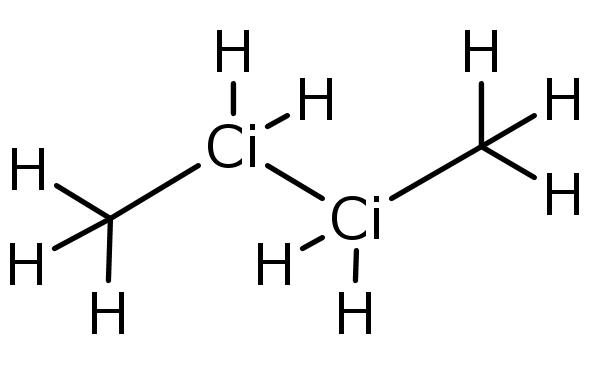
\includegraphics[width=5cm, height=3cm]{visuals/butane} % 300 dpi
\end{center}

We will set up a butane example and measure the bond distances in the
CH3- and CH2-groups. There are three atom types: Methyl-carbon
(\texttt{C} in CH3), methylene-carbon (\texttt{Ci} in CH2, i stands for
``inner'') and Hydrogen (\texttt{H}). The butane data file is build
accordingly and the field \texttt{neighbors=4} is added. The ensemble
provided with the tutorial files consists of $5\times 5\times 5$ butane
molecules with a density of \SI{2.71}{\kilogram\per\cubic\meter}. The
unit system used is kcalpermole.

\begin{lstlisting}[caption=Header of the .data file]
# ATOMDATA Id type x=3 u=3 neighbors=4
\end{lstlisting}

When setting up the \texttt{butane.potentials} file, begin with Lennard
Jones interaction, which should additionally work in between molecules.
Tremolo-X handles Lennard Jones in bonded molecules in a way, that the
potential is \emph{not} calculated among direct neighbors. However for
large molecules, like proteins, intramolecular interaction should be
considered: These are controlled via the settings \texttt{sigma14} and
\texttt{epsilon14}, as they take effect from the fourth bond on, hence
the naming.

As for the bonded potentials we use \texttt{bonds}, \texttt{angles} and
\texttt{torsions}. The angle potential, like the bonds, is harmonic
(linear restoring force for angle displacement from an optimal value)
and the torsional potential is expressed as cosine series expansion. All
parameters are taken from the AMBER94 force field. For the literal
definition of the potential terms see the potentials-section in this
manual (\ref{sse:bondedpotentials}).

\begin{lstlisting}[escapechar=', caption=Excerpt from the
    .potentials file]
bonds {
  bond: particle_type1=C, particle_type2=Ci, bond_type=harmonic, k_b=310, r_0=1.526;
  '[\dots]'
};

angles {
  angle: particle_type1=C, particle_type2=Ci, particle_type3=Ci, angle_type=harmonic, k_th=40, theta_0=109.5;
  '[\dots]'

torsions {
  torsion: particle_type1=H, particle_type2=C, particle_type3=Ci, particle_type4=H, torsion_type=cosine, k_1=1.4, delta_1=0, n_1=3, mult=1;
  '[\dots]'

};
\end{lstlisting}

The simulation \texttt{\$PROJECTNAME.parameters} are a simple \texttt{NVE} ensemble
with verlet propagator and initial temperature of \SI{0}{\celsius}. In the
\texttt{analyze} section bond distance measurement is set up. It
doesn't matter whether the measured pair is bonded in means of the
\texttt{neighbors} field: Every pair with specified types undershooting the
specified threshold (in this particular case \SI{180}{\pico\meter} for C--C and
\SI{140}{\pico\meter} for H--C) are considered bonded and their Ids written to the
\texttt{\$PROJECTNAME.info.bonds} (vis) file. The mean value of bond lengths of any 
pair of types requested in the \texttt{\$PROJECTNAME.parameters} file is written to 
the \texttt{\$PROJECTNAME.generalmeas} file.

\begin{lstlisting}[caption=Excerpt from the .parameters file]
    analyze {
        bond: measure=on, meanmeasure=off, vis=off;
        bondDistances {
            bondDistance: particle_type1=Ci, particle_type2=Ci, distance=1.8;
            bondDistance: particle_type1=C, particle_type2=Ci, distance=1.8;
            bondDistance: particle_type1=Ci, particle_type2=H, distance=1.4;
            bondDistance: particle_type1=C, particle_type2=H, distance=1.4;
        };
\end{lstlisting}

As we can see the mean values oscillate around a constant, so there is
no time dependant development. We assume the ensemble is equilibrated
after 20 time units and compare the mean of the mean values for any
available pair and get following results:

\begin{center}
    \begin{tabular}{ccc}
        \toprule
        Bond & Distance/\si{\pico\meter} & $r_0$/\si{\angstrom} \\
        \midrule
        \texttt{C}--\texttt{Ci} & 152.7(1) & 1.526 \\
        \texttt{Ci}--\texttt{Ci} & 152.7(2) & 1.526 \\
        \texttt{C}--\texttt{H} & 109.1(1) & 1.09 \\
        \texttt{Ci}--\texttt{H} & 109.08(9) & 1.09 \\
        \bottomrule
    \end{tabular}
\end{center}

There are no differences in the bond length within statistical error and
the values match the $r_0$-Parameter because the same parameters were
used for both, inner and outer, carbon atom types. The nearest neighbors
of the atoms (spatial configuration) are not taken into account thus
leading to an identical bond distance.

\subsection{Exercises}
\begin{itemize}
    \item Increase the temperature or lower the bond strength and
        observe the magnitude of the oscillation.
    \item Alter the equilibrium distance $r_0$.
\end{itemize}

\section{Tersoff potential and stress}
After we successfully introduced basic bonded and non-bonded force fields, this
chapter shows how to use a bond order potential to determine Young's Modulus of
a single graphene sheet. Instead of defining fixed individual neighbors, the
potential function will determine the spatial configuration of surrounding
carbon atoms by itself. This way the \texttt{graphene.data} file looks rather trivial,
the force field parameters for \texttt{graphene.potentials} are taken directly
from \cite{tersoff88a}:

\begin{lstlisting}
tersoff {
    tersoffparticle: particle_type=C0, A=32115.7, B=7990.67, lambda=3.4879, mu=2.2119, beta=1.5724e-07, n=0.72751, c=38049, d=4.3484, h=-0.57058, R=1.95, S=2.1;
};
\end{lstlisting}

Just like in \ref{tutorial:barostat} an \texttt{NPT}-ensemble is used, but this time
additionally to the external pressure we also support a custom stress tensor,
which stretches the domain in \texttt{xx}-direction with linearly increasing
strength, starting from $0$ in the beginning up to $1e5\,\frac{[F]\,[V]}{[A]}$\footnote{\textbf{F}orce, \textbf{V}olume and \textbf{A}rea.
For a detailed explanation of the volume term see chapter~\ref{output:stress}}
(\texttt{kcalpermole} units). At this time note that the stress value is not
given in units of pressure, as one would expect, but contains a surplus
$V$-Term.  The volume can usually be derived from the domain dimensions, but
particularly in this tutorial we have to \emph{decide} how much volume a single
graphene sheet has. Also the box vectors need to be changed individually, so we
will choose \texttt{standard} constraints (\texttt{isotropic} constraints would be
infeasible due to the coupling of the constraints).

\begin{lstlisting}
barostat {
    parinello: state=on, f_mass=500;
    constraint: type=standard;
    constraintmap: xx=1, xy=0, xz=0, yx=0, yy=1, yz=0, zx=0, zy=0, zz=0;
    constantpressure: state=on, Pressure=1.45742e-05;

    stresstensor: [time, stress, interpolation, xx, xy, xz, yy, yz, zz =
        (0, 0, linear, 1, 0, 0, 0, 0, 0),
        (200, 1e5, linear, 1, 0, 0, 0, 0, 0)];
};
\end{lstlisting}

Stress and strain are measured automatically if \texttt{outm} is set. However
if you are interested in the stress distribution along individual particles you
need to use the \texttt{local\_stress}-feature:

\begin{lstlisting}
analyze {
    local_stress: localstress=on;
};
\end{lstlisting}

If activated, the beta column in the visual .pdb output contains per particle
stress, which can be visualized with an external tool like VMD-Viewer (not
covered by this tutorial). Due to limitations of the PDB-format the numerical
value is clipped at $99.99\,\frac{[F]\,[V]}{[A]}$.

After the simulation has been finished, the output is analyzed by plotting a
stress-strain diagram. The strain is defined as the length change relative to
the initial box \texttt{xx}-length $L_0$: $\epsilon(L) = \frac{L-L_0}{L0}$.
The argument will be the $43^{rd}$ column in the file \texttt{graphene.mbox}, which
is the domain length in \texttt{xx} direction. The stress is read
from column 31 in the same file and divided by the volume of the graphene sheet, which is the product of
\texttt{xx} length (column 43), \texttt{yy} length (column 44) and
\textit{height}, which has to be chosen by the user. We set $height=3.7
\mathring{A}$, the inter layer distance in graphite. Note that since we pull,
the stress value from the file is negative. With this information we can now
use gnuplot to create the diagram and fit a slope against the initial
section, representing the elastic zone where Hook's Law applies. This slope is
the Young's Modulus.

\begin{lstlisting}
gnuplot> L0 = 48.19683
gnuplot> epsilon(L) = (L-L0)/L0
gnuplot> plot 'graphene.mbox' using (epsilon($43)):(-$31/($43*$44*3.7))

gnuplot> f(x) = E*x
gnuplot> fit [0:0.04] f(x) 'graphene.mbox' using (epsilon($43)):(-$31/($43*$44*3.7)) via E
\end{lstlisting}

\begin{figure}[h]
    \centering
    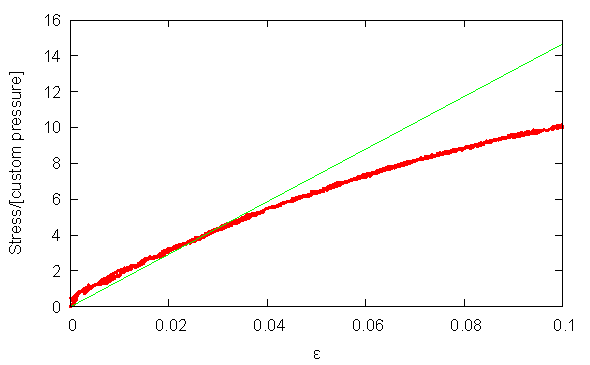
\includegraphics{visuals/graphene.pdf}
    \caption{Stress-strain diagram of monolayer graphene (red) with green slope fit.}
\end{figure}

We obtain $E=146.7(5)\,\frac{[F]}{[A]}$, in SI-units $1019(3)\,\textrm{GPa}$, which
sufficiently reproduces the measurement of $1\,\textrm{TPa}$ in~\cite{egraphene}.

\subsection{Exercises}
\begin{itemize}
    \item Change the pull direction to \texttt{yy}. Are there differences?
    \item Alter the force progression:
    \begin{itemize}
        \item Increase the simulation length by factor ten.
        \item Add a $100\,[t]$ relaxation time at the beginning ($\sigma=0$).
        \item Increase the maximum stress at the end of the simulation by factor five.
    \end{itemize}
    Create a new stain-stress plot -- is there a difference in the fit quality
    ($\chi^2_\textrm{d.o.f.}$ and parameter error as supplied by gnuplot)?
\end{itemize}

\section{Long ranged potentials 1 - Halley's Comet with $\mathbf{N^2}$}
This tutorial covers how to set up simulation to use long ranged
potentials like gravity or the coulomb potential. In either case the
potential's distance characteristic is $\propto\ 1/x$ and any kind of
cutoff introduces significant errors on the forces and with them error
in macroscopical observables.

The simpelest way to deal with these kind of potentials is using an
ordinary pair potential. As stated earlier the potential should not be
cut off but has to to fit the linked cell structure of the domain. With
only a few particles it is adequate to run the whole simulation in a
single cell, the performance drops quadratically with the particle
number. In this example we simulate our solar system and calculate when
Halley's Comet runs through its perihelion point next time (as of time
of writing, year 2013).

To obtain handy numbers we set up following unit system in the
\texttt{.tremolo} file:

\begin{center}
    \begin{tabular}{ccc}
        \toprule
        Quantity & Unit & Equals \\
        \midrule
        Length & \SI{1.496e11}{\meter} & \si{\astronomicalunit} \\
        Time & \SI{86400}{\second} & \siday \\
        Mass & \SI{1e23}{\kilogram} & $\approx m_\mathrm{Earth} / 100$ \\
        \bottomrule
    \end{tabular}
\end{center}

For the \texttt{.data} file we use positions (relative to the
Barycenter) and velocities obtained from JPL HORIZONS for sixty
astronomical objects of our solar system including the most massive
ones. The data represents the state of the solar system on December
19th, 2012.

Tremolo-X doesn't support ``gravity'' literally, but since the potential
is identic to the coulomb potential disregarding the force constant we
set up a coulomb simulation with adapted \texttt{epsilon0inv}. It can
easily be calculated with Gnu Units:
\begin{lstlisting}
> units -t G "(m*1.496e11)**3 / (kg*1e23 * (s*86400)**2)"
1.4881216e-11
\end{lstlisting}
Note that the value needs to be multiplied by $-1$ so equally named
``charges'' attract each other.

We use an NVE ensemble with \texttt{verlet} propagator,
\SI{0.05}{\siday} \texttt{timestep} and \SI{100}{\siyear} \texttt{endtime},
``temperature'' and ``pressure'' can't be applied on the experimental
conditions. Also it would not be accurate to wrap around the
gravitational forces at the borders of the solar system as it is
preferred when homogenous systems are observed, so we choose the domain
to three times larger than the solar system, place it in the center
(done with a \texttt{INPUTCONV SHIFT} directive in the data file) and
set \texttt{leaving} boundary conditions (particles passing the border
are removed):

\begin{lstlisting}
lcs: cellrcut = 80.0;

domain {
    size: type=cube, size=240;
        border: bt_xlow=leaving, bt_xhigh=leaving, bt_ylow=leaving,
    bt_yhigh=leaving, bt_zlow=leaving, bt_zhigh=leaving;
};
\end{lstlisting}

A single linked cell will be large enough to contain the whole
ensemble. This is not practical for large scale molecular dynamics
because it can't be paralellized, however unless a more sophisticated
method like SPME (covered in the next section) is used, it is the only
way to obtain accurate results using long ranged potentials.

The \texttt{coulomb} section is set up thusly:

\begin{lstlisting}
coulomb {
    permittivity: epsilon0inv=-1.4881216e-11;
    n2spline: state=on, r_cut=80, r_l=70, i_degree=5;
};
\end{lstlisting}

The \texttt{n2spline} solver calculates the force for every pair and cuts
off beyond \SI{70}{\astronomicalunit} with a spline taper (like
\texttt{ljspline}). The cutoff is chosen large enough to contain the
whole solar system so the forces will be exact. If \texttt{n2spline} is
used in molecular dynamics with small cutoff the spline interpolation
guarantees conservation of energy but the forces will be off their exact
result due to the characterstic of the potential.

The bond distance measurement covered earlier is used to measure the
distance between Halley's Comet/Earth and the Barycenter:
\begin{lstlisting}[escapechar=']
output {
'[\dots]'
    analyze {
        bond: measure=on, meanmeasure=off, vis=off;
        bondDistances {
            bondDistance: particle_type1=Barycenter, particle_type2=Earth, distance=80;
            bondDistance: particle_type1=Barycenter, particle_type2=Halley, distance=80;
        };
    };
};
\end{lstlisting}

Finally we set up the objects in the \texttt{.potentials} file. To
calculate the gravity potential with the coulomb solver we need to set
the ``charge'' of the particle to its mass. The Barycenter is included
as pseudo particle with mass 1 and no charge -- this way it won't be
affected by any force and stay central.

After running the simulation we extract the time to the minimum of
$|\vec r_\mathrm{Barycenter}-\vec r_\mathrm{Halley}|$ by plotting the
first and fourth column of the \texttt{.generalmeas} file. It's 17750
time units (days), so the next perihelion is 25th July 2061, slightly
deviant to the value computed with HORIZONS: 28th July. This relative
difference of 0.02\% is caused by the simplification of the solar system
to sixty objects and the resulting difference in the local density. The
minima of the Earth--Barycenter distance are \SI{365.24}{\siday} apart
which matches the definition of the tropical year.

\subsection{Excercises}
\begin{itemize}
    \item Remove any particle but Sun, Jupiter, Barycenter and Halley
        and compare the relative error of the perihelion.
    \item Only remove Jupiter from the original setup and compare the
        relative error, observe planetary trajectories and the length of an
        earth year.
\end{itemize}


\section{Long ranged potentials 2 - Sodium chloride with SPME}
This part covers a typical usage scenario of coulomb forces in molecular
dynamics with more than just a few particles. To maintain a good
performance with a large $N$ the potential is seperated into a short
ranged part, which is calculated in a linked cell fashion as before, and
a long ranged part, which is calculated by Ewald summation in fourier
space, to take into account farther particles. In comparison to the Fast
Multipole Method, which abstracts groups of far particles into a single
one, this way is espacially suitable for periodic systems, like an ionic
crystal: In this example we are going to simulate solid NaCl and measure
its radial distribution functions. The system
of units used is \texttt{kcalpermole}.

In the \texttt{.potentials}-file we set up the short ranged interactions
using the Tosi Fumi\cite{tosifuminacl} Potential, which has shown to
produce accurate results with this kind of system. The starting
configuration in the data file is an NaCl-structure with small random
offset for each atom at \SI{20}{\celsius}.

We set up an \texttt{NPT}-ensemble in the \texttt{.parameters} file with
\SI{1000}{\hecto\pascal} pressure maintained by the Parrinello-Barostat with
isotropic constraint (the crystal is cubic) and
Nose-Hoover-Thermostat for fixed temperature. In the
\texttt{coulomb}-section we specify the parameters for the
\texttt{spme}-method and a force constant using the vacuum permittiviy:

\begin{lstlisting}
coulomb {
    permittivity: epsilon0inv=332;
    spme: state=on, r_cut=9.0, G=0.32, i_degree=5, cellratio=4;
};
\end{lstlisting}

Up to \texttt{r\_cut}, which is the short ranged part of the potential,
the force is evaluated locally (restricted to neighbored cells) and pair
wise, as if \texttt{n2spline} was used. From there it is approximated by
bell curves with splitting coefficient
\texttt{G}, which is inverse to the standard deviation $\sigma$, and
applied on a mesh, which is created by splitting the linked cell
\texttt{cellratio} times (rounded upward to the next power of two).
\texttt{G} should be kept at \SIrange{0.24}{0.35}{\angstrom^{-1}}.

In the \texttt{analyze}-section we set up the measurement of the radial
distributions of all atom types:

\begin{lstlisting}[escapechar=']
output {
'[\dots]'
    analyze {
        radial: measure=on, meanmeasure=off, vis=off, r_cut=9.0, n_bin=50;
        radialdistribution {
            radialdist: particle_type1=Na, particle_type2=Na;
            radialdist: particle_type1=Na, particle_type2=Cl;
            radialdist: particle_type1=Cl, particle_type2=Cl;
        };
    };
};
\end{lstlisting}

The value of \texttt{r\_cut} has to be within the \texttt{lcs: cellrcut}
limits, just like the \texttt{r\_cut} of the potentials.

Since we now use the SPME method, we have to use a parellel version
of Tremolo-X, since the SPME method is not implemented sequentially.
Nevertheless you can unse the SPME method and start the parallel 
version with a single process.

\emph{If you do not know how to run the parallel version of Tremolo-X,
please check chapter \ref{FirstParallelSteps} and \ref{running_tremolo}.}

\subsection{Excercises}
\begin{itemize}
    \item Compare the radial distribution histograms from first (ideal
        NaCl structure) and last timestep.
    \item Decrease/Increase the temperature and observe the differences
        in the radial distribution.
\end{itemize}

\section{Melting point of Sodium Chloride}
In the previous Tutorial the basics for simulating an ionic crystal
using the Coulomb- and Tosi-Fumi-Potential have been covered while this
one shows how to determine the melting point of NaCl, which is a common
application of molecular dynamics. From the different methods described
in \cite{nacl_melting} we are going to use the \emph{Voids method}: A
series of NaCl lattices with increasing defect concentration (removed
atoms) is simulated using an NPT-ensemble with temperature timeline.
Starting with an ideal lattice, which is a hypothetical, defect free
state at \SI{0}{\kelvin}, the temperature at which the lattice breaks
(``melting point'') is significantly overestimated because the
activation energy for this transition is very high. By removing atoms
from the crystal it becomes labile and the lattice breaks easily if the
temperature is high enough, lowering the activation energy to start the
melting process. If the defect concentration is too high the crystal
rearranges back into a more stable configuration, increasing the
observed melting point. This process leads to a reduced volume which has
to be compensated for, using a barostat. Therefore if the measured melting point is
plotted against defect concentration one can see that the measured melting point
decreases quickly with increasing defect concentration at first and then
oscillates around the actual melting point, which can be obtained by
calculating the mean value.

A tricky aspect is how to observe the melting point: Liquid and solid
state can be discriminated using the MSD-measurement, potential energy,
density, radial distribution or bond length, usually indicated by a rapid
slope change which can be seen if these measurements are plotted.
Preliminary studies have shown that observing the bond lenght is the
easiest to interpret while very accurate option in this particular
example: As the crystal heats up the bond lenght increases linearily
until the crystal breaks and the bond distances relaxes rapidly. The
obsverved melting point $T_m$ is the temperature at maximum bond lenght.

The simulation setup is similar to the previous tutorial apart from the
thermostat settings and more measurement options in the
\texttt{nacl.parameters} file:

\begin{lstlisting}[extendedchars=\true, inputencoding=utf8x]
thermostat {
    timeline: state=on, [time, temperature, interpolation =
    (0, 0.5822, linear), # 20C°
    (100, 0.5822, linear),
    (1000, 2.9255, linear)]; # 1200C°

    nosehoover: state=on, F_Mass=800;
};
\end{lstlisting}
\todo{Buchstabendreher beim Gradzeichen im PDF/Text fixen
(Encodingproblem mit lstlisting).}

With these settings the temperature is held constant at
\SI{20}{\celsius} for 100 time units and then lineary increased to
\SI{1200}{\celsius} at the end of the simulation (1000 time units).

\begin{lstlisting}
bond: measure=on;
bondDistances {
    bondDistance: particle_type1=Na, particle_type2=Cl, distance=4.0;
};
\end{lstlisting}

Every Na--Cl-pair with a distance less than or equal to \SI{4}{\angstrom} is
considered bonded and contributes to the mean distance written to
\texttt{nacl.generalmeas}.

When carrying out a series of simulations it is handy to make use of the
\texttt{defaultpath}-option in \texttt{nacl.tremolo}. The simulation is
organized into a root directory which contains any file but
\texttt{.data} and \texttt{.tremolo} and subdirectories containing only
these, whith individual \texttt{nacl.data} containing an increasingly
more defective crystal. The individual \texttt{nacl.tremolo} files look
like this

\begin{lstlisting}
global: defaultpath="../nacl";
global: projectname="nacl";
global: comment="NaCl";
global: systemofunits=kcalpermole;
\end{lstlisting}

with the \texttt{defaultpath} set to the parent directory and nacl as
basename, so tremolo looks for \texttt{\emph{nacl}.potentials} and so
forth. The subdirectories are named after the relative count of cells
containing a (single) pair defect. A single cell contains 8 atoms, so
the resulting defect concentration is $dirname/4$.

After the simulations are done the times at which the bond lenght peaks
are read from \texttt{nacl.generalmeas} and the temperature at this time
is looked up in \texttt{nacl.ekin}, fourth column.

Plotting $T_m$ against defect concentration results in following graph:

\begin{figure}[h]
    \centering
    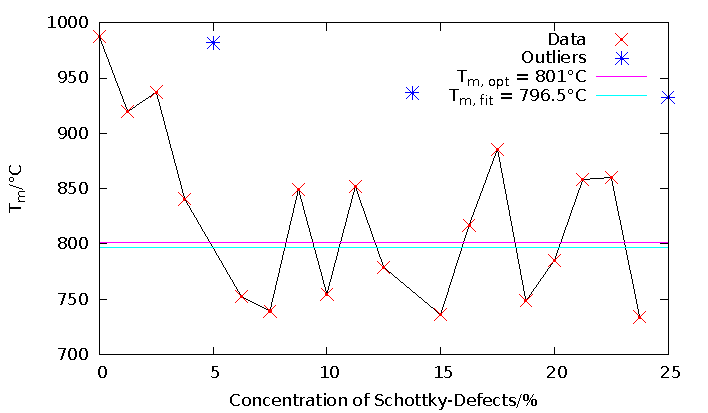
\includegraphics{visuals/nacl_melting.pdf}
    \caption{Melting points at different defect concentrations.
        $T_\textrm{m, opt}$ is the melting point according to literature,
        $T_\textrm{m, fit}$ is the mean value of the oscillating region.
        The black dot-connecting line and outliers are for visualization
    purposes only.}
\end{figure}

The oscillating region starts after \SI{7.5}{\percent}, the resulting
mean value differs by \SI{4.5}{\kelvin} from the exact value of
\SI{801}{\celsius}, which is a relative error as low as
\SI{0.6}{\percent}.

\section{The EAM potential - Observing phase transition in Metall}

The ``embedded atom method'' (EAM) is a standard potential used in the analysis of metalls and alloys.
They are used quite successfully in the investigation of fractures, surface reactions martensite-austenite transitions
and phasechanges in condensed matter, nano particles and thin films.

In this tutorial lesson we will demonstrate the use of the EAM potential and how a phase transition
can be analyzed with Tremolo-X. 
We will heat a Fe-Ni nanoparticle from 100 K to 800 K and observe it changing its lattice structure from
bcc to fcc/hcp.

In order to use EAM potentials, the user must have a file with EAM parameters in the format ``eam/fs'' (a generalized EAM type by Finnis-Sinclaire) or 
in the ``eam/alloy'' format, which is slightly modified from DYNAMO setfl file formats. For a detailled description of the EAM formats supported, please
check the appropriate section \ref{potentials:eam}

The unit system of the eam parameters file determines the units which need to be used throughout the simulation. As a result in this example SI units will be used.
The respective entries for iron and nickel particle values in the potential file are consequently:
\begin{lstlisting}
particles	{
	particle:	particle_type=Fe,	element_name=Fe,	
			sigma=1.0,		epsilon=0.0,	
			sigma14=1.0,		epsilon14=0.0,	
			mass= 9.2732785e-26,	
			free=3,
			charge=0;
	particle:	particle_type=Ni,	element_name=Ni,	
			sigma=1.0,		epsilon=0.0,	
			sigma14=1.0,		epsilon14=0.0,	
			mass=9.7462664e-26,	
			free=3,
			charge=0;
	};	
\end{lstlisting}

and subsequently we specify the format (``alloy'' format) and the filename in the following way:
\begin{lstlisting}
eam    {
         setfl:     file="Fe-Ni-MeyerEntel-1995.eam.alloy";        
       };
\end{lstlisting}


In the parameter file we need to specify the following:

\begin{lstlisting}
integration: type=dynamics;
########## Section Domain:
domain {
      size:    type=cube, size=60.0e-10;
      border:  bt_xlow=periodic,
               bt_xhigh=periodic,
               bt_ylow=periodic,
               bt_yhigh=periodic,
               bt_zlow=periodic,
               bt_zhigh=periodic;
		};
########## Section Ensemble and Propagator:
dynamics {
	ensemble:	ensemble=NVT;
	propagator,	verlet:	delta_T=1.0e-15,	endtime=8.0e-11,	timeinteps=1e-07,	maxiteration=100;
	thermostat	{
		berendsen:  state=on,
                            T_Interval=1.0e-15;
		timeline:   state=on,
                      [time, temperature, interpolation=
		      (0,        1.3806503e-21, linear), # 100K / 7.2429638e+22 K
	              (1e-14,	 1.3806503e-21,	linear),
		      (7.56e-11, 1.1045202e-20,	linear), # 800K
		      (8.0e-11,	 1.1045202e-20,	linear)];
			};
	 };
########## Section Solver and Parallelization:
lcs:	cellrcut=5.6001e-10; 
########## Section Output Measurement:
output	{
	Outvis:	T_Start=0, T_Delta=5.0e-13, Step_Delta=100;
	Outm:	T_Start=0, T_Delta=1.0e-15, Step_Delta=100;
	Outmm:	T_Start=0, T_Delta=5.0e-14, T_Deltam=4.0e-14, Step_Delta=20, Step_Deltam=10;
	Outdata: T_Start=0, T_Delta=10.0e-13, Step_Delta=50;
	energy:	measure=on,	meanmeasure=off;
	analyze	{
	  radial: measure=on, meanmeasure=off, vis=on, r_cut=5.6001e-10, n_bin=56;
		radialdistribution	{
	            radialdist: particle_type1=Ni, particle_type2=Ni;
		    radialdist: particle_type1=Ni, particle_type2=Fe;
        	    radialdist: particle_type1=Fe, particle_type2=Fe;
                     };
                   };
	};
\end{lstlisting}

Note that while we use SI units, the temperature has a scaling prefactor, which needs to be accounted for when setting the thermostat. While we use periodic boundaries, those will not be relevant to our simulation, as we 
set the simulation domain to a cube of 60$\angstrom$, whereas the nanoparticle has a radius of 20 $\angstrom$. Thus no interaction with or across the domain boundaries is present.

We now can run the simulation.After having run the simulation, we can take a look at the potential energy curve and notice that its slope changes around 4.64e-11s into the simulation. It is at this time that
the transformation takes place.

We will now analyze the radial distribution of the sample at the beginning of the simulation, during the melting phase and after the transition phase.
For this we will use the tool ``CalcRadialHist'' delivered with Tremolo-X.

By calling 
\begin{lstlisting}
CalcRadialHisto eam.histogram 5e-15 15.3e-15 0.0 5.6e-10 3.0e-10 1 56 545 2196 216000 3.0e-10 > RadialHist
\end{lstlisting}
we average the radial distribution over the time interval from 5 to 15 fs and write the results to the file {\tt RadialHist}.
The same can be done for the time intervals 4e-11s to 4.3e-11s and  5e-11s to 5.3-11s. When those three distributions are compared,
we observe, that around 4e-11s the original configuration has been severly melted, but that around 5e-11s the atoms have rearanged themselves, 
which can be seen from the clearly shifted peaks in the radial distribution function.






%Bibliographie
%\nocite{*}
\bibliography{./bib/Tremolo_Manual.bib}
\bibliographystyle{plain}

%\clearpage
%\listoffigures
%\listoftables


%\printindex
%\IfDefined{printindex}{\printindex}
%\IfDefined{printnomenclature}{\printnomenclature}




%% Dokument ENDE %%%%%%%%%%%%%%%%%%%%%%%%%%%%%%%%%%%%%%%%%%%%%%%%%%%%%%%%%%
\end{document}

